\documentclass[a4paper]{article}

\usepackage{amsmath}
\usepackage{amssymb}
\usepackage{stellar}
\usepackage{parskip}
\usepackage{fullpage}
\usepackage{wrapfig}
\usepackage{tikz}

\usetikzlibrary{arrows}
\usetikzlibrary{decorations.pathreplacing}
\usetikzlibrary{cd}

\title{Analisi II}
\author{Paolo Bettelini}
\date{}

% libri
% pagani-salsa
% fusco-marcellini-sbordone 

\begin{document}

\maketitle
\tableofcontents

\section{Spazi metrici}

\subsection{Definizioni}

L'insieme vuoto e l'insieme \(X\) sono aperti e chiusi.

\sproposition{}{
    L'unione di aperti non numerabile è aperta, mentre l'intersezione è aperta solo se finita.
}

\sproof{}{
    Per dimostrare quest'ultima lo facciamo su due insiemi e il resto è per induzione.
    Prendiamo un punto nell'interezione e prendiamo le due bolle dentro gli insiemi centrate
    nel punto. Siccome hanno lo stesso centro la loro intersezione è sempre una bolla di raggio
    il minore fra i due.
}

La metrice discreta può generare una bolla che è un singoletto.

\sproposition{}{
    L'unione di chiusi finiti è chiusa. L'intersezione qualsiasi è chiusa.
}

Ogni singoletto è chiuso. Per dimostrarlo mostriamo che nel complementare
esiste una bolla che non interseca il punto (vero per proprietà di Hausdorff).

Tutti i punti di accumulazione sono dei punti aderenti.
Tutti i punti di un sottoinsieme sono aderenti per il sottoinsieme.
Ogni punto o è di accumulazione o è isolato.

Se \(x_0\) è aderente ad E, \(x_0\) può essere un punto di E oppure no.
Se \(x_0\) è punto di accumulazione per E, in ogni bolla centrata in \(x_0\) cadono inifniti punti.

\sproposition{}{
    \(E^\circ\) è aperto. \(E\) è aperto se e solo se \(E = E^\circ\).
    \(E^\circ\) è il più grande aperto contenuto in \(E\).
    
    \(\overline{E}\) è chiuso. \(E\) è chiuso se e solo se \(E = \overline{E}\).
    La chiusura di \(E\) è il più piccolo chiuso contenente \(E\).
}

\sproof{per l'interno}{
    Dimostriamo che \(E^\circ\) è aperto. Sia \(x_0 \in E^\circ\).
    un punto interno ad \(E\), quindi esiste una bolla centrata in tale punto che è contenuta in \(E\).
    Prendiamo un altro punto \(y\) in questa bolla. Possiamo costruire una inner bolla centrata in \(y\)
    con un raggio sufficientemente piccolo da rimanere nella bolla più grande. Quindi il punto \(y\)
    è a sua volta interno, quindi tutta la bolla centrata in \(x_0\) è in \(E^\circ\) e quindi è aperto.
    
    Dimostriamo ora che se \(E\) è aperto allora \(E=E^\circ\) (l'altra implicazione è ovvia).
    Per fare ciò dimostriamo che \(E^\circ\) è il più grande aperto in \(E\).
    Osserviamo che \(E^\circ\) fa parte della famiglia degli aperti di \(X\)
    contenuti in \(E\). Sia \(A\) un aperto contenuto in \(E\). VOglio dimostrare che \(A \subseteq E^\circ\).
    Sia \(x_0 \in A\). \(A\) èunione di bolle quindi esiste unr aggio tale che la
    bolla centrata in \(x_0\) di tale raggio è contenuta in \(A\) che è contenuto in \(E\).
    Quindi, \(x_0\) è interno ad \(E\) e \(x_0 \in E^\circ\) e \(A \subseteq E^\circ\).
    Supponiamo ora che \(E\) sia aperto. Allora \(E\) fa parte della famiglia degli aperti
    di \(X\) contenuti in \(E\). Devo avere \(E \subseteq E^\circ\).
    Dato che \(E^\circ \subseteq E\) allora \(E^\circ = E\).
}

% lezione 2

Dire che un insieme è dentro in un altro significa dire che la sua chiusura coincide con l'insieme.
Tipo la chiusura di Q è R quindi Q è denso in R.


\sdefinition{Limitato}{
    Se è contenuto in una bolla
}

\sdefinition{Diametro}{
    è il sup della metrica su tutte le coppie.
}

\sdefinition{Ricoprimento}{
    Sia \(E\) un sottoinsieme di uno spazio metrico \(X\). Una famiglia
    \[
        \{G_\alpha\}_{\alpha \in A}
    \]
    è un ricoprimento apert di \(E\) se
    \[
        E \subseteq \bigcup_{\alpha \in A} G_\alpha
    \]
}

\sdefinition{Sottoricoprimento}{
    Un Sottoricoprimento di 
    \[
        \{G_\alpha\}_{\alpha \in A}
    \]
    è una sottofamiglia di \(G_\alpha\)
    tale che continua a ricoprire. Cioè ne scarto alcuni ma deve comunque rimanere
    una copertura.
}

\sdefinition{Compatto}{
    Uno spazio metrico \(X\) è compatto se ogni ricoprimento aperto di \(E\)
    ammette un sottoricoprimento finito.
}

Ogni insieme finito è compatto.


\stheorem{}{
    Sia  \(X\) uno spazio metrico e \(E\) un sottoinsieme di \(X\) compatto.
    \begin{enumerate}
        \item \(E\) è limitato;
        \item \(E\) è chiuso;
        \item Ogni sottoinsieme infinito di \(E\) ha almeno un punto di accumulazione in \(E\).
    \end{enumerate}
}

\sproof{}{
    \begin{enumerate}
        \item Consideriamo \(\{B_1(x) \,|\, x\in E\}\) che è un ricoprimento aperto di \(E\).
        Siccome \(E\) è compatto esiste un sottoricoprimento finito aperto di \(E\), ossia
        \(x_1, \ldots, x_n \in E\) tali che
        \[
            E \subseteq \bigcup_{i=1}^n B_1(x_i)
        \]
        Posto
        \[
            R = 1 + \max_{i=1,\ldots,n} d(x_i, x_1)
        \]
        Allora la bolla di raggio \(R\) centrata in \(x_1\) contiene \(E\), quindi \(E\) è limitato.
        \item Supponiamo che non sia chiuso. Allora esiste \(y\in E'\) ma \(y\notin E\).
        Vogliamo costruire un ricoprimento aperto di \(E\) che non ammette sottoricoprimento finito.
        Sia \(r(x) = \frac{1}{2} d(x,y)\) per ogni \(x\in X\).
        Se \(x\in E\) allora \(r(x) > 0\) perchè \(y\notin E\).
        Abbiamo il ricoprimento
        \[
            \{B_{r(x)}(x) \,|\, x\in E\}
        \]
        Ma per la compattezza esisterebbe un sottoricoprimento finito, cioè \(x_1, \ldots, x_n \in E\) tali che
        \[
            E \subseteq \bigcup_{i=1}^n B_{r(x_i)}(x_i)
        \]
        Sia ora \(R = \min_{i=1,\ldots,n} r(x_i)\). Allora \(R > 0\) e la bolla \(B_R(y)\)
        non interseca nessuna delle \(B_{r(x_i)}(x_i)\), assurdo poiché \(y\) è punto di accumulazione.
        \item Sia \(F\) un sottoinsieme infinito di \(E\). Supponiamo che \(F\) non abbia punti di accumulazione in \(E\).
        Allora ogni punto di \(E\) ha una bolla che interseca \(F\) in al più un punto.
        Queste formano un ricoprimento aperto di \(E\).
        Ma se esistesse un sottoricoprimento finito, \(F\) sarebbe finito, assurdo.
    \end{enumerate}
}

\sproposition{}{
    Sia \(E \subseteq X\) compatto. Se \(F \subseteq E\) è chiuso allora \(F\) è compatto.
}
\sproof{}{
    Sia \(\{G_\alpha\}_{\alpha \in A}\) un ricoprimento aperto di \(F\).
    Dobbiamo aggiungere degli insiemi aperti per coprire il resto.
    Siccome \(F\) è chiuso, \(X \setminus F\) è aperto.
    Quindi \(\{G_\alpha\}_{\alpha \in A} \cup \{X \setminus F\}\) è un ricoprimento aperto di \(E\).
    Per la compattezza di \(E\) esiste un sottoricoprimento finito, che escludendo \(X \setminus F\)
    è un sottoricoprimento finito di \(F\).
}

% ESERCIZIO
Se \(F\subseteq X\) è chiuso, ed \(E\subseteq X\) è compatto, allora \(F \cap E\) è compatto.

\stheorem{Teorema dell'intersezione finita}{
    Sia \(\{E_\alpha\}_{\alpha \in A}\) una famiglia di compatti tale che
    ogni intersezione finita è non vuota. Allora
    \[
        \bigcap_{\alpha \in A} E_\alpha \neq \emptyset
    \]
}

\sproof{}{
    Supponiamo che l'intersezione sia vuota. Allora
    e sia \(E_{\overline{\alpha}}\) un compatto fissato nella famiglia.
    \begin{align*}
        &E_{\overline{\alpha}} \cap \left(
            \bigcap_{\alpha \neq \overline{\alpha}} E_\alpha
        \right) = \emptyset \\
        &\implies
        E_{\overline{\alpha}} \subseteq
        \left(
            \bigcap_{\alpha \neq \overline{\alpha}} E_\alpha
        \right)^c
        =
        \bigcup_{\alpha \neq \overline{\alpha}} E_\alpha^c
    \end{align*}
    \(\{E_\alpha^c\}_{\alpha \neq \overline{\alpha}}\) è un ricoprimento aperto di \(E_{\overline{\alpha}}\).
    Esistono quindi \(\alpha_1, \ldots, \alpha_n \neq \overline{\alpha}\)
    tali che \begin{align*}
        &E_{\overline{\alpha}} \subseteq \bigcup_{i=1}^n E_{\alpha_i}^c
        = \left(
            \bigcap_{i=1}^n E_{\alpha_i}
        \right)^c \\
        &\implies
        E_{\overline{\alpha}} \cap \left(
            \bigcap_{i=1}^n E_{\alpha_i}
        \right) = \emptyset
    \end{align*}
    assurdo. % lightning
}

\scorollary{caso particolare}{
    Sia \(\{E_n\}_{n\in \mathbb{N}}\) una famiglia di compatti tale che
    \[
        E_{n+1} \subseteq E_n
    \]
    Allora
    \[
        \bigcap_{n\in \mathbb{N}} E_n \neq \emptyset
    \]
}

\stheorem{Teorema di Heine-Borel}{
    Sia \(E \subseteq R^n\) con la metrica euclidea. Allora \(E\) è compatto se e solo se
    \(E\) è chiuso e limitato.
}

\slemma{}{
    Sia \(\{I_k\}_{k\in \mathbb{N}}\) una famiglia di intervalli
    \(I_k = [a_k, b_k]\) tali che \(I_k \supseteq I_{k+1}\).
    Allora 
    \[
        \bigcap_{k\in \mathbb{N}} I_k \neq \emptyset
    \]
}

\sproof{}{
    Gli intervalli sono annidati, quindi \(a_k\) è crescente e \(b_k\) è decrescente e \(a_k \leq b_k\).
    In particolare \(a_k \leq b_i\). Consideriamo l'insieme \(E = \{a_k \,|\, k\in \mathbb{N}\}\).
    \(E\) è limitato superiormente, e ammette supremum \(x\).
    Per definizione \(x \geq a_k\). Ma \(a_k \leq b_i\) per tutte le \(i\).
    Quindi, \(x \leq b_i\) per ogni \(i\). Allora
    \[
        x \in I_n \implies x \in \bigcap I_k
    \]
}

\sdefinition{}{
    Siano \(a,b \in \mathbb{R}^n\) con \(a_i < b_i\) per ogni \(i=1,\ldots,n\).
    Un rettangolo chiuso è il prodotto cartesiano
    \[
        [a_1, b_1] \times [a_2, b_2] \times \ldots \times [a_n, b_n]
    \]
    che indichiamo con \([a,b]\).
}

\slemma{}{
    Sia \(\{R_k\}_{k\in \mathbb{N}}\) una famiglia di rettangoli chiusi
    tali che \(R_k \supseteq R_{k+1}\) per ogni \(k\).
    Allora
    \[
        \bigcap_{k\in \mathbb{N}} R_k \neq \emptyset
    \]
}

\sproof{}{
    Siccome
    \[
        R_k = I_{k,1} \times I_{k,2} \times \ldots \times I_{k,n}
    \]
    possiamo applicare il primo lemma e quindi
    \[
        \exists y_i \in \bigcap_{k\in \mathbb{N}} I_{k,i}
    \]
    Il punto \(y = (y_1, \ldots, y_n)\) è in ogni \(R_k\).
}

\slemma{Lemma 3}{
    In \(\mathbb{R}^n\) con la metrica euclidea
    ogni rettangolo è compatto.
}

\sproof{Lemma 3}{
    Sia \(R = [a,b]\) un rettangolo e supponiamo che non sia compatto.
    Sia \(\{G_\alpha\}_{\alpha \in A}\) un ricoprimento aperto di \(R\)
    che non ammette sottoricoprimento finito.
    Vogliamo adesso dimezzare ambo i lati (quindi \(n\) tagli).
    Abbiamo adesso \(2^n\) rettangoli.
    \[
        [a_i, b_i] = [a_i, c_i] \cup [c_i, b_i], \quad
        c_i = \frac{a_i + b_i}{2}
    \]
    Il diametro di \(R\) è \(||b-a||\).
    Il diametro di ogni rettangolo ottenuto è la metà.
    Almeno uno di questi rettangoli ha la proprietà di non ammettere sottoricoprimento finito.
    Lo chiamiamo \(R_1\).
    Iterando il procedimento otteniamo una successione di rettangoli
    \[
        R \supseteq R_1 \supseteq R_2 \supseteq \ldots
    \]
    con diametro che tende a zero e che non ammettono sottoricoprimento finito, il diametro
    di \(R^k\) è dato da \(\frac{1}{2^k} ||b-a||\).
    Per il lemma precedente esiste \(x \in \bigcap_{k\in \mathbb{N}} R_k\).
    Siccome \(R_k \subseteq R\) per ogni \(k\), \(x \in R\).
    Siccome \(\{G_\alpha\}_{\alpha \in A}\) è un ricoprimento di \(R\),
    esiste \(\alpha_0 \in A\) tale che \(x \in G_{\alpha_0}\).
    \(G_{\alpha_0}\) è aperto, quindi esiste \(r > 0\) tale che
    \(B_r(x) \subseteq G_{\alpha_0}\).
    Scegliamo \(k\) sufficientemente grande tale che \(2^{-k} ||b-a|| < r\).
    Ma il diametro di \(R_k\) è minore di \(r\), quindi \(R_k \subseteq B_r(x)\).
    Quindi \(R_k \subseteq G_{\alpha_0}\), assurdo perchè \(R_k\) non ammette sottoricoprimento finito.
}

\sproof{Heine-Borel}{
    Dobbiamo dimostrare solo che se \(E\) è chiuso e limitato allora è compatto.
    Siccome \(E\) è limitato esiste \(M\) tale che \(||x|| < M\) per ogni \(x \in E\).
    Quindi,
    \[
        E \subseteq [-M, M] \times [-M, M] \times \ldots \times [-M, M] = R
    \]
    \(E\) è un chiuso contenuto in un compatto, quindi è compatto.
}

\stheorem{Teorema di Bolzano-Weierstrass}{
    Ogni sottoinsieme infinito e limitato di \(\mathbb{R}^n\) ha almeno un punto di accumulazione.
}

\sproof{Teorema di Bolzano-Weierstrass}{
    % todo semplice una riga
}

\sdefinition{Insiemi separati}{
    Sia \((X, d)\) uno spazio metrico e \(A,B\subseteq X\) due sottoinsiemi.
    Diciamo che \(A\) e \(B\) sono separati se
    \[
        A \cap \overline{B} = \emptyset \land \overline{A} \cap B = \emptyset
    \]
}

Devono sicuramente essere disgiunti, ma non basta.
Serve che nessun punto di uno dei due insiemi è punto di accumulazione
dell'altro.

\sdefinition{}{
    Sia \((X, d)\) uno spazio metrico e \(E\subseteq X\). \(E\) è connesso
    se non può essere scritto come unione di due sottoinsiemi non vuoti e separati.
}

I sottoinsiemi connessi di \(\mathbb{R}\) sono tutti e soli gli intervalli.

Uno spazio metrico è connesso se e solo se l'unico sottoinsieme non vuoto
di \(X\) che è anche aperto e chiuso è \(X\) stesso. (Dimostrazione per esercizio).

\(R^n\) con la metrica euclidea è connesso. (Dimostrazione per esercizio non proprio banale).

\subsection{Successioni in spazi metrici}

Mettere la definizione di convergenza ma con \(d(x_m,y) < \varepsilon\).
Oppure \(x_m \in B_\varepsilon(y)\).

In particolare la successione metrica converge se e solo se \(d(x_m, y) \to 0\)
secondo la convergenza reale.

Il limite è unico per proprietà di Hausdorff.

\sproposition{}{
    Sia \((X,d)\) uno spazio metrico e \(E \subseteq X\) e sia \(y\) un punto di accumulazione
    per \(E\). Allora esiste una successione \(\{x_n\} \subseteq E \setminus \{y\}\)
    che converge ad \(y\).
    In particolare, \(E\) è chiuso se e solo se per ogni successione \(\{x_n\} \subseteq E\)
    che converge ad \(y\) allora \(y \in E\).
}

\sproof{}{
    Dato che \(y\in E'\), \(\forall x_m \in \mathbb{N}\), esiste \(x_m\) tale che
    \(x_m \in B_{\frac{1}{m}}(y) \cap E\) e \(x_m \neq y\).
    La successione così costruita converge ad \(y\).
    Infatti, \(d(x_m, y) < \frac{1}{m} \to 0\).
}

\sproposition{}{
    Sia \((X,d)\) uno spazio metrico e sia \(\{x_n\}\) una successione convergente in \(X\).
    Una condizione necessaria per la convergenza è che ogni sottosuccesione converga allo stesso limite.
    La condizione sufficiente è che ogni sottosuccessione ammetta una sottosuccessione
    che converge allo stesso limite.
}

\sdefinition{Compattezza sequenziale}{
    Uno spazio metrico \(X\) è sequenzialmente compatto se ogni successione in \(X\)
    a valori in \(E\) ammette una sottosuccessione convergente ad un punto di \(E\). 
}

\sproposition{Equivalenza compattezza}{
    \(E\) is compact is and only if \(E\) is sequentially compact.
}

Questa c'è solo negli spazi metrici.

\sproof{}{
    \iffproof{
        Sia \(\{x_n\}\) una successione in \(E\).
        Consideriamo \(F = \{x_n \,|\, n\in \mathbb{N}\}\).
        Se \(F\) è finito, esiste un elemento che compare infiniti volte
        e la successione costante converge a tale elemento.
        Se \(F\) è infinito, per la compattezza \(F\) ammette un punto di accumulazione, \(y\in E\).
        Costruiamo una sottosuccessione che converga ad \(y\).
        Scegliamo \(x_m\) tale che \(d(x_m, y) < 1\).
        Scegliamo \(x_{m_2}\) tale che \(d(x_{m_2}, y) < \frac{1}{2}\) e \(m_2 > m_1\), e così via.
        La sottosuccessione così costruita converge ad \(y\) in quanto \(d(x_{m_k}, y) < \frac{1}{k} \to 0\).
    }{
        XXX
    }
}

Ogni successione convergente è di Cauchy.

Per esempio con la metrica discreta una successione è convergente se e solo se è definitamente costante,
che è equivalente ad essere di Cauchy, quindi è completo.

Nel caso dei razionali nei reali con metrica euclidea, consideriamo la radice di due che è un punto di accumulazione
per i razionali. Esiste una successione di razionali che converge a radice di due, quindi è di Cauchy.
Ma essa non può convergere in Q, altrimenti convergerebbe anche in R e avrebbe due limiti.
Tuttavia è una successione di Cauchy in Q perché è convergente in R e quindi è di Cauchy in R.
(La condizione è la medesima). Quindi Q non è completo.

\sdefinition{Spazio completo}{
    Uno spazio metrico \((X,d)\) è completo se ogni successione di Cauchy in \(X\)
    converge ad un punto di \(X\).
}

\stheorem{}{
    \(R^n\) con la metrica euclidea è completo.
}

\sproof{}{
    Sia \(\{x_n\}\) una successione di Cauchy in \(R^n\).
    Scriviamo \(E_n = \{x_k \,|\, k \geq n\}\).
    Notiamo che \(E_n \supseteq E_{n+1}\).
    Ponendo la chiusura \(\overline{E_n} \supseteq \overline{E_{n+1}}\).
    Inoltre, \(E_n\) è limitato e \(\text{diam} E_n \to 0\).
    Infatti, dato \(\varepsilon > 0\) esiste \(N\) tale che per ogni \(m,n \geq N\)
    \(d(x_n, x_m) < \varepsilon\).
    Notiamo inoltre che
    \[
        \text{diam} E_n = \sup\{d(x_m,x_k)\} < \varepsilon
    \]
    Dimostrazione per esercizio vale che \(\text{diam} F = \text{diam} \overline{F}\).
    Quindi, \(\text{diam} \overline{E_n} \to 0\).
    Adesso \(\{\overline{E_n}\}\) è una successione di compatti in quanto chiusi e limitati, annidati.
    Quindi \[
        E \triangleq \bigcap_{n\in \mathbb{N}} \overline{E_n} \neq \emptyset
    \]
    Siccome \(\text{diam} E = 0\) o è vuoto o contiene un solo punto, quindi contiene un solo punto \(E = \{y\}\).
    Mostriamo che \(x_n \to y\).
    Abbiamo \(d(x_n, y) \leq \text{diam} \overline{E_n} \to 0\).
}

\stheorem{}{
    Sia \((X, d)\) uno spazio metrico compatto.
    Allora \(X\) è completo.
}

\sproof{}{
    Sia \(\{x_n\}\) una successione di Cauchy in \(X\).
    Siccome è compatto è compatto per successioni, quindi esiste una sottosuccessione
    \(\{x_{n_k}\}\) che converge ad un punto \(y \in X\).
    Mostriamo che \(x_n \to y\).
    Dato \(\varepsilon > 0\) esiste \(N_0\) tale che per ogni \(m,n \geq N_0\)
    \(d(x_n, x_m) < \frac{1}{2}\varepsilon\).
    Per la convergenza di \(\{x_{n_k}\}\) esiste \(K\) tale che per ogni \(k \geq K\)
    \(d(x_{n_k}, y) < \frac{1}{2}\varepsilon\).
    Scegliamo \(\overline{N} = \max\{N_0, n_K\}\).
    Allora per ogni \(n \geq \overline{N}\) si ha
    \[
        d(x_n, y) \leq d(x_n, x_{n_K}) + d(x_{n_K}, y) < \frac{1}{2}\varepsilon + \frac{1}{2}\varepsilon = \varepsilon
    \]
}

%%%% 1 ott


%%% ????
Sia \(X\) uno spazio metrico completo, \(Y \subseteq X\).
\(Y\) è completo se e solo se \(Y\) è chiuso in \(X\).

\stheorem{}{
    \(E\) sequenzialmente comaptto implica \(E\) compatto.
}

\sproof{}{
    Sia \(\{G_\alpha\}_{\alpha \in A}\) un ricoprimento aperto di \(E\).
    Esiste \(\delta > 0\) tale che \(\forall x \in E\) esiste \(\overline{\alpha}\)
    tale che \(B_\delta(x) \subseteq G_{\overline{\alpha}}\).
    \begin{enumerate}
        \item \emph{claim 1:} \(\forall m \in \mathbb{N}\), esiste \(x_m\) tale che
            \(B_{1/m}(x_m)\) non è sottoinsieme di \(G_\alpha\) per tutte le \(\alpha\).
            \(\{x_m\}\) è una successione in \(E\) e quindi posso estrarre una sottosuccessione convrgente
            \(x_{m_k} \to p \in E\). Esiste \(\hat{\alpha}\) tale che \(p \in G_{\hat{\alpha}}\).
            \(G_{\hat{\alpha}}\) è aperto e quindi esiste una \(\varepsilon > 0\)
            tale che \(B_\varepsilon(p) \in G_{\hat{\alpha}}\).
            Ma \(x_{m_k} \to p\) quindi con \(k\) sufficientemente grande
            \[B_{1/m_k}(x_{m_k}) \subseteq B_\varepsilon(p) \subseteq G_{\hat{\alpha}}\]
            che è assurdo lightning.
        \item \emph{claim 2:} \(E\) è contenuto nel'unione di un numero finito di bolle di raggio
            \(\delta\) centrate in punto di \(E\).
            Per assurdo, sia \(x_1 \in E\). Sicuramente \(B_\delta(x_1)\)
            non ricopre \(E\) quindi esiste \(x_2 \in E \backslash B_\delta(x_1)\).
            Ma assieme \(B_\delta(x_1) \cup B_\delta(x_2)\) non ricoprono \(E\),
            quindi esiste un \(x_3 \in E \backslash (B_\delta(x_1) \cup B_\delta(x_2))\)
            e così via. La successione \(\{x_m\}\) deve ammettere una sottosuccessione
            convergente. Ma \(d(x_i, x_j) \geq \delta\) se \(i \neq j\) quindi la sucessione
            \(\{x_m\}\) non è di Cauchy Lightning.
            Quindi \(E \subseteq B_\delta(x_1) \cup B_\delta(x_2) \cup \cdots\).
    \end{enumerate}
}

In realtà abbiamo mostrato anche la terza.

\stheorem{}{
    Sia \(X\) uno spazio metrico. Sono equivalenti:
    \begin{enumerate}
        \item \(X\) è compatto;
        \item \(X\) è sequenzialmente compatto;
        \item \emph{limit point compact:} ogni sottoinsieme infinito
        di \(X\) ha almeno un punto di accumulazione.
    \end{enumerate}
}

Solo negli spazi metrici.

\subsection{Funzioni}

\sdefinition{}{
    Siano \((X_1, d_1), (X_2, d_2)\) due spazi metrici e sia \(E \subseteq X_1\).
    Sia \(f \colon E \to X_2\) e \(p \in E'\).
    Diciamo che \(l\in X_2\) è limite di \(f(x)\) per \(x\to p\) e diciamo
    \[
        \forall \varepsilon > 0, \exists \delta > 0 \,|\, x \in E
        \land 0 < d_1(x_1, p) < \delta \implies d_2(f(x), l) < \varepsilon
    \]
    Equivalentemente \(\forall \varepsilon >0\) esiste \(\delta > 0\)
    tale che \[f((B_\delta(p) \cap E) \backslash \{p\}) \subseteq B_\varepsilon(l)\]
}

\sproposition{}{
    Sia \(f\colon E \subseteq X_1 \to X_2\).
    Allora \(f(x) \to l\) per \(x\to p\) se e solo se \(f(x_n) = l\)
    per ogni successione \(\{x_n\}\) tale che \(x_n \in E\)e \(x_n \neq p\)
    per tutte le \(n\) e \(x_n \to p\).
}

Valgono i medesimi teoremi tipo l'unicità del limite e i teoremi di permanenza del segno, confronto etc.

\sproposition{}{
    Sia \(f \colon E \subseteq X \to \mathbb{R}^n\) per \(n > 1\).
    Allora
    \[
        f(x) \to l \iff f_i(x) \to l_i
    \]
    per \(x \to p\).
}

\sproof{Sketch}{
    Conderiamo la norma per tutte le \(i\)
    \begin{align*}
        |f_i(x)-l_i| \leq ||f(x) - l|| \leq \sum_k |f_k(x) - l_k|
    \end{align*}
}

\sdefinition{Continuità}{
    Siano \((X_1, d_1), (X_2, d_2)\) due spazi metrici,
    \(f \colon E \subseteq X_1 \to X_2\), \(p \in E\).
    Diciamo che \(f\) è \emph{continua} in \(p\)
    se \(\forall \varepsilon > 0\) esiste \(\delta > 0\) tale che
    \[\forall x \in E \cap B_\delta(p) \implies f(x) \in B_\varepsilon((f(p)))\]
    Euivalentemente \(\forall \varepsilon > 0\) esiste \(\delta > 0\)
    tale che \(x\in E\) e \(d_1(x,p) <\delta\) implica che \(d_2(f(x), f(p)) < \varepsilon\).
    Oppure ancora \((f(B_\delta(p) \cap E)) \subseteq B_\varepsilon(f(p))\).
}

Se \(p\) è un punto isolato di \(E\) allora \(\exists r > 0\)
tale che \(B_r(p) \cap E = \{p\}\). Scegliendo \(\delta \leq r\)
la definizione di continuità è automaticamente soddisfatta.
Se \(p\) non è i solato, allora è un punto di accumulazione per \(E\).
In questo caso \(f\) è continua in \(p\) e vale che \(f(x) \to f(p)\) per \(x\to p\).

\sproposition{}{
    \(f\) è continua in \(p\) se e solo se
    \[
        \lim_{x\to p} f(x_n) = f(p)
    \]
    per ogni successione \(\{x_n\}\) tale che \(x_n \in E\)
    per tutte le \(n\) e \(x_n \to p\).
}

\sdefinition{}{
    Sia \(f \colon E \subseteq X_1 \to X_2\). Diciamo che \(f\) è continua nell'insieme \(E\)
    se \(f\) è continua in ogni punto di \(E\).
}

\sproposition{}{
    Siano \((X_1, d_1), (X_2, d_2)\) spazi metrici e sia \(f \colon X_1 \to X_2\).
    Allora \(f\) è continua in \(X\) se e solo se \(f^{-1}(V)\) è aperto in \(X_1\)
    per tutti i \(V\) aperti in \(X_2\).
}

\sproof{}{
    \iffproof{
        Sia \(V\) un aperto di \(X_2\). Se \(f^{-1}(V) = \emptyset\)
        in questo caso abbiamo finito. Altrimenti,
        sia \(p \in f^{-1}(V)\), cioè \(f(p) \in V\).
        Essendo \(V\) aperto, riesco a trovare \[ B_\varepsilon(f(p)) \in V \]
        Ma \(f\) è continua quindi riesco anche a trovare \(\delta>0\) tale che
        \[
            f(B_\delta(p)) \subseteq B_\varepsilon(f(p))
        \]
        Quindi \(B_\delta(p) \subseteq f^{-1}(V)\) quindi \(p\) è un punto interno a
        \(f^{-1}(V)\). Per l'arbitrarietà di \(p\) segue che \(f^{-1}(V)\) è aperto.
    }{
        Sia \(p \in X\) e dimostriamo che \(f\) è continua in \(p\).
        Sia \(\varepsilon > 0\) fissato. \(B_\varepsilon(f(p))\)
        è un aperto di \(X_2\). \(f^{-1}(B_\varepsilon(f(p)))\) è un aperto di \(X_1\)
        e \(p \in f^{-1}(B_\varepsilon(f(p)))\) e quindi esiste \(\delta > 0\)
        tale che
        \[
            B_\delta(p) \subseteq f^{-1}(B_\varepsilon(f(p)))
        \]
        cioè
        \[
            f(B_\varepsilon(p)) \subset B_\varepsilon(f(p))
        \]
        che è la definizione di continuità.
    }
}

Siccome \(f^{-1}(E^c) = \left(f^{-1}(E)\right)^c\) allora \(f\)
è continua se e solo se \(f^{-1}(C)\) è chiuso in \(X_1\)
per ogni chiuso in \(C \in X_2\). Molto utile.

In generale le funzioni continue non mandano aperti in aperti.
Per esempio \(f \colon \mathbb{R} \to \mathbb{R}\)
data da \(x \to x^2\).
Abbiamo che
\[
    f((-1,1)) = [0,1)
\]

\sdefinition{Funzione aperta}{
    Una funzione viene detta \emph{aperta}
    se \(f(U)\) è aperto in \(X_2\) per tutti gli insiemi \(U\) aperto om \(X_1\).
    Analogamente funzione chiusa.
}

Sia \(f \colon (X, d) \to \mathbb{R}^n\) con \(n>1\)
è continua se e solo se tutte le sue componenti sono continue.

\sproposition{}{
    Siano \((X_1, d_1), (X_2, d_2)\)
    spazi metrici, \(f \colon X_1 \to X_2\) una funzione continua.
    Se \(X_1\) è compatto, allora \(f(X_1)\) è compatto.
}

\sproof{}{
    Sia \(\{G_\alpha\}_{\alpha \in A}\) un ricoprimento aperto di \(f(X_1)\).
    Consideriamo \(\{f^{-1}(G_\alpha)\}_{\alpha \in A}\) che sono degli aperti.
    Queste preimmagini sono un ricoprimento di \(X_1\),
    che è compatto e quindi posso estrarre un sottoricoprimento finito
    \(f^{-1}(G_{\alpha_1}), \cdots, f^{-1}(G_{\alpha_n})\).
    Vogliamo mostrare che \(\{G_{\alpha_1}, \cdots, G_{\alpha_n}\}\)
    sono un ricoprimento di \(f(X_1)\).
    \[
        f(X_1) = f \left(
            \bigcup_{i=1}^n f^{-1}( G_{\alpha_i})
        \right)
        = \bigcup_{i=1}^n f\left(
            f^{-1}(G_{\alpha_i})
        \right)
        \subseteq \bigcup_{i=1}^n G_{\alpha_i}
    \]
}

\stheorem{Teorema di Weierstrass}{
    Sia \((X,d)\) uno spazio metrico compatto e sia
    \(f \colon X \to \mathbb{R}\) una funzione continua.
    Allora, \(\exists x_1, x_2 \in X\) tali che
    \[
        f(x_1) \leq f(x) \leq f(x_2), \quad \forall x \in X
    \]
    cioè \(f\) possiede massimo e minimo assoluto.
}

\sproof{Teorema di Weierstrass}{
    \(f(X)\) è compatto in \(\mathbb{R}\), quindi è chiuso e limitato.
    Siccome limitato, \(f(X)\) ammette infimum e supremum reali.
    Siccome \(\inf f(x)\) e \(\sup f(x)\)
    appartengono a \(\overline{f(x)}\) e \(f(x)\) è chiuso, appartengono allora ad \(f(X)\)
    e quindi sono massimi e minimi.
}

\stheorem{Teorema da compatto ad Hausdorff}{
    Siano \((X_1, d_1), (X_2, d_2)\) spazi metrici
    con \(X_1\) compatto e \(f \colon X_1 \to X_2\) continua.
    Allora, \(f\) è chiusa.
}

In realtà questo funziona con domini compatti e codomini di Hausdorff.

\sproof{Teorema da compatto ad Hausdorff}{
    Sia \(C\) un chiuso di \(X_1\).
    Voglio dimostrare che \(f(C)\) è un chiuso di \(X_2\).
    Sappiamo che \(C\) è chiuso in un compatto, quindi è compatto.
    La funzione è continua e quindi \(f(C)\) è compatto.
    Siccome i compatti sono chiusi allora è chiuso.
}

\scorollary{}{
    Sia \(f \colon (X_1, d_1) \to (X_2, d_2)\) continua, \(X_1\) compatto e
    \(f\) biunivoca. Allora, \(f^{-1}\) è continua.
}

\sproof{}{
    Dobbiamo mostrare che \((f^{-1})^{-1}(C)\) è chiuso per ogni \(C\) chiuso di \(X_2\).
    Ma questo coincide con \(f(C)\) che è chiusa per il teroema da compatto ad Hausdorff.
}

\stheorem{}{
    Sia \(f\colon (X_1, d_1) \to (X_2, d_2)\) continua e sia \(E \subseteq X\) connesso.
    Allora \(f(E)\) è connesso.
}

\sproof{}{
    Supponiamo che \(f(E)\) non sia connesso. Esistono quindi
    due sottoinsiemi non vuoti disgiunti e separati tali che
    \[
        f(E) = A \cup B
    \]
    Poniamo \(F = f^{-1}(A) \cap E\) e \(G = f^{-1}(B) \cap E\).
    Sicuramente \(F,G \neq \emptyset\) e \(E = F\cup G\). Vogliamo mostrare che \(E\) e \(G\)
    sono separati.
    Siccome \(A \subseteq \overline{A}\) vale anche \(f^{-1}(A) \subseteq f^{-1}(\overline{\overline{A}})\).
    L'applicazione \(f\) è continua e la chiusura di \(A\) è un chiuso.
    Quindi la preimmagine del chiuso \(\overline{A}\) è un chiuso.
    Consideriamo ora \[\overline{F} \subseteq \overline{f^{-1}(A)} = f^{-1}(\overline{A})\]
    perché \(f\) è continua se \(\overline{A}\) è chiuso.
    Quindi \(\overline{F} \subseteq f^{-1}(\overline{A})\) che implica
    \(f(\overline{F}) \subseteq \overline{A}\). D'altro canto \(f(G) \subseteq B\)
    e \(\overline{A} \cap B \neq 0\), e quindi \(\overline{F} \cap G \neq 0\)
    perché altrimenti vi sarebbe un elemento sia in \(\overline{A}\) che in \(B\).
    Dovrebbe essere \(f(x) \in \overline{A}\) e \(f(x) \in B\) lightinng.
    Analogamente si dimostra che \(F \cap \overline{G} = \emptyset\)
    cioè abbiamo scritto \(E\) come unione di due sottoinsiemi non vuoti e separati.
    Ma \(E\) è connesso lightning.
}

\sdefinition{}{
    Siano \((X_1, d_1),(X_2, d_2)\) spazi metrici e \(f\colon X_1 \to X_2\).
    Allora \(f\) è uniformemente continua se
    \(\forall \varepsilon > 0\), esiste \(\delta > 0\)
    tale che \(\forall x,y \in X_1\)
    \[
        d_1(x, y) < \delta \implies d_2(f(x), f(y)) < \varepsilon
    \]
}

\stheorem{Theorema di Heine-Cantor}{
    Siano \((X_1, d_1),(X_2, d_2)\) spazi metrici e 
    \(f\colon (X_1, d_1) \to (X_2, d_2)\)
    continua e \(X_1\) compatto.
    Alorra, \(f\) è uniformemente continua.
}

La dimostrazione è la medesima rispetto al caso banale.

\sdefinition{Funzione di Lipschitz}{
    Siano \((X_1, d_1),(X_2, d_2)\) spazi metrici,
    \(f\colon X_1 \to X_2\).
    Diciamo che \(f\) è \emph{lipschitz-continua} o \emph{lipschitziana}
    se \(\exists \alpha > 0\) tale che
    \[
        d_2(f(x), f(y)) \leq \alpha d_1(x,y)
    \]
    per tutte le \(x,y \in X_1\).
}

\sproposition{}{
    Se \(f\) è Lipschitz-continua, allora è uniformemente continua.
}

\sdefinition{}{
    Siano \((X_1, d_1),(X_2, d_2)\) spazi metrici e 
    \(f\colon (X_1, d_1) \to (X_2, d_2)\).
    Diciamo che \(f\) è una \emph{contrazione} se
    \(f \in \text{Lip}_\alpha(X_1, X_2)\) con \(\alpha < 1\).
}

Se il supremum è finito, allora questa è la miglior costante di Lipschitz (in generale)
\begin{align*}
    \sup_{x\neq y} \frac{|f(x)-f(y)|}{|x-y|}
\end{align*}

\sexample{}{
    Consideriamo \(f \colon \mathbb{R} \to \mathbb{R}\)
    data da \(f(x) = x^2\). Non è di lipschitz inquanto non è uniformemente continua.
    Per mostrarlo possiamo dire
    \begin{align*}
        |f(x)-f(y)| &= |x^2 - y^2| = |x+y| \cdot |x-y|
    \end{align*}
    Se restringessimo il dominio di questa funzione ad un intervallo limitato,
    allora sarebbe di Lipschitz, per il supremum.
}

\sproposition{}{
    Sia \(f\colon I \subseteq \mathbb{R} \to \mathbb{R}\) differenziabile.
    Allora, \(f \in \text{Lip}_\alpha(I, \mathbb{R})\)
    se e solo se \(|f'(x)| \leq \alpha\) per tutte le \(x\).
}

\sproof{}{
    \iffproof{
        Cominciamo con
        \begin{align*}
            |f'(x)| &= \left| \lim_{t\to 0} \frac{f(x+t)-f(x)}{t}\right| \\
            &= \lim_{t\to 0} \left| \frac{f(x+t)-f(x)}{t}\right| \\
            &= \lim_{t\to 0} \frac{|f(x+t)-f(x)|}{|t|} \\
            &\leq \lim_{t\to 0} \frac{\alpha |x+t-x|}{|t|} = \alpha
        \end{align*}
        Possiamo togliere il limite dal modulo in quanto il modulo è una funzione continua.
    }{
        Per il teorema di Lagrange esiste \(\theta \in (\min\{x,y\}, \max\{x,y\})\)
        \begin{align*}
            f(x) - f(y) &= f'(\theta) (x-y) \\
            |f(x) - f(y)| &= |f'(\theta)|\cdot |x-y| \\
            &\leq \alpha|x-y|
        \end{align*}
    }
}

\sexercise{}{
    Per quali \(a \leq b\) la funzione \(f(t) = 1 + t - \arctan(t)\)
    è una contradizione in \([a,b]\).
    Stabiliamo quindi se la derivata è limitata
    \begin{align*}
        f'(t) = 1 + \frac{1}{1 + t^2} = \frac{t^2}{1 + t^2}
    \end{align*}
    notiamo quindi che \(0 \leq f'(t) \leq 1\). Quindi è sicuramente lipschitziana.
    Notiamo allora che
    \[
        \sup_{\mathbb{R}} |f'(t)| = 1 = \alpha
    \]
    Quindi per far sì che \(\alpha < 1\) dobbiamo limitare il dominio ad un intervallo limitato.
    Quindi \(-\infty < a \leq b < \infty\).
    Porta l'intervallo \([a,b]\) in sè?
    Siccome la funzione è crescente porta intervalli a intervalli
    di estremi \(f(a)\) e \(f(b)\). Mi basta quindi imporre
    che \(f(a) \geq a\) e \(f(b) \leq b\). Abbiamo quindi
    \begin{align*}
        \begin{cases}
            1 + a - \arctan a \geq a \\
            1 + b - \arctan b \leq b
        \end{cases}
        =
        \begin{cases}
            \arctan a \leq 1 \\
            \arctan b \geq 1
        \end{cases}
    \end{align*}
    e quindi \(a \leq \tan 1 \leq b\).
    Notiamo che \(f(\tan 1) = \tan 1\) quindi è un punto fisso
    per il teorema delle contrazioni.
}

\sexample{}{
    Sia \(v \in \mathbb{R}^n\) e consideriamo
    \(f\colon \mathbb{R}^n \to \mathbb{R}\) data da
    \(f(x) = v \cdot x\).
    Dobbiamo studiare \(|f(x) - f(y) = |v\cdot x - v \cdot y|\)
    usando la bilinearità del prodotto scalare ottengo
    \(|v\cdot (x-y)|\). Per Cacuhy-Schwarz
    \[
        |v\cdot (x-y)| \leq ||v|| \cdot ||x-y||
    \]
    che è quindi di Lipschitz.
}

\stheorem{Teorema di Banach-Cacciopoli o delle contrazioni}{
    Sia \((X, d)\) uno spazio metrico completo
    e sia \(f \colon X \to X\) una contrazione.
    Allora \(\exists_{=1}\, x \in X\) tale che \(f(x) = x\).
}

Le ipotesi sono necessarie.
Togliamo per esempio la completezza e consideriamo quindi \(X=(0, +\infty)\)
con la contrazione \(f(x) = x/2\). Questa contrazione non ha punti fissi.
Togliamo invece l'ipotesi che sia una contrazione.
Richiediamo solamente che sia una contrazione debole, cioè
\[
    d_2(f(x), f(y)) \leq f_1(x,y)
\]
Consideriamo \(X = [0, +\infty)\) e prendiamo
\(f(t) = t + e^{-t}\). 
La derivata è \(f'(t) = 1-e^{-t}\) che è nulla nell'origine
e poi tende ad \(1\) dal sotto.
Chiaramente non ci sono punti fissi in quanto \(f(t)=t\) è come dire \(e^{-t} = 0\).

\sproof{}{
    Cominciamo mostrando l'esistenza del punto fisso.
    Sia \(x_0 \in X\) un punto fissato e
    consideriamo la successione \(x_{n+1} = f(x_n)\).
    \begin{enumerate}
        \item Mostriamo che \(\{x_n\}\) è di Cauchy, quindi siccome lo spazio è completo
        converge. Dobbiamo mostrare che \(d(x_n, x_m)\) tende a zero quando \(n,m\) crescono.
        Consideriamo inizialmente
        \begin{align*}
            d(x_{n+1}, x_n) &= d(f(x_n), f(x-{n-1})) \leq \alpha d(x_n, x_{n-1}) \\
            &= \alpha d(f(x_{n-1}), f(x_{n-2})) \leq \alpha^2 d(x_{n-1}, x_{n-2}) \\
            &\leq \alpha^n d(x_1, x_0)
        \end{align*}
        Calcoliamo ora la distanza generica e usiamo la disuguaglianza triangolare
        ripetutamente per ogni step
        \begin{align*}
            d(x_{n+k}, d_n) &\leq \sum_{i=0}^{k-1} d(x_{n+k-i}, d_{n+k-i-1}) \\
            &\leq d(x_1, x_0) \sum_{i=0}^{k-1} \alpha^{n+k-i} \\
            &= \alpha^n d(x_1, x_0) \sum_{i=0}^{k-1} \alpha^{n+k-i-1} \\
            &= \alpha^n \frac{\alpha^k - 1}{\alpha - 1} d(x_1, x_0) \\
            &= \frac{\alpha^n}{1 - \alpha} d(x_1, x_0) \to 0
        \end{align*}
        Per sbarazzarci di \(k\) (siccome vogliamo \(k\) arbitrario e il \(\varepsilon\)
        nella definizione di Cauchy deve essere uniforme rispetto ad esso)
        maggioriamo la somma parziale della serie geometrica
        con il valore della serie geometrica. Siccome \(0 < \alpha < 1\) il termine non esplode
        e la serie geometrica converge.
        \item Detto \(x\) il limite di \(\{x_n\}\) mostriamo che è un punto fisso di \(f\).
        Consideriamo il limite per \(n\to \infty\)
        \[
            \lim_{n \to \infty} f(x_n) = f\left(\lim_{n \to \infty} x_n\right)
            = f(x)
        \]
        perché \(f\) è continua.
    \end{enumerate}
    Mostriamo ora l'unicità del punto.
    Supponiamo che \(x,y\) siano due punti fissi. Vogliamo mostrare che \(d(x,y) = 0\).
    Abbiamo
    \begin{align*}
        d(x,y) &= d(f(x), f(y)) \leq \alpha d(x,y)
        (1-\alpha) d(x,y) &\leq 0
    \end{align*}
    siccome \(1-\alpha > 0\) ciò succede solo se \(d(x,y) = 0\).
}

Abbiamo notato che
\[
    d(x_{n+k}, x_n) \leq \frac{\alpha^n}{1 - \alpha} d(x_1, x_0)
\]
Con \(k \to \infty\) otteniamo
\[
    d(x, x_n) \leq \frac{\alpha^n}{1 - \alpha} d(x_1, x_0)
\]
quindi tende al punto fisso in maniera esponenziale.

Denotiamo \(f^n = f \circ f \cdots f\).
Se \(f\) è una contrazione, una qualsiasi sua iterazione è anch'essa una contrazione.
\begin{align*}
    d(f(f(x)), f(f(y))) \leq \alpha d(f(x), f(y)) \leq \alpha^2 d(x,y)
\end{align*}
Per induzione segue il resto. In generale la costante è \(\alpha^n\).
Ci chiediamo se nel caso in cui \(f\) non sia una contrazione, una sua iterata lo possa essere.

\sexample{}{
    Per esempio \(f(x) = \cos x\), che non è una contrazione in quanto il supremum
    della derivata è \(1\). Invece, \(\cos(\cos(x))\) ha derivata
    \[
        \sin(\cos(x)) \cdot \sin
    \]
    Il suo modulo è dato da
    \[
        |\sin(\cos(x))| \cdot |\sin x|
        \leq \sin(1) < 1
    \]
    Il secondo termine può solamente essere maggiorato da \(1\), mentre il secondo,
    siccome \(-1 \leq \cos(x) \leq 1\), può essere maggiorato da \(\sin 1\).
    Quindi è una contrazione.

    Con questo possiamo per esempio mostrare che il coseno ha un punto fisso,
    siccome una sua iterata è una contrazione.
}


\scorollary{Indebolimento del teorema delle contrazioni: teorema delle iterate contrazioni}{
    Sia \((X, d)\) uno spazio metrico completo e sia
    \(f \colon X \to X\) un'applicazione tale che \(\exists n \in \mathbb{N}\)
    tale che \(f^n\) sia una contrazione. Allora \(\exists_{=1}\, x\in X\)
    tale che \(f(x)=x\).
}

\sproof{}{
    Mostriamo che i punti fissi di \(f\) (che sono uno solo) sono i punti fissi di \(f^n\).
    Sia \(x\) un punto fisso di \(f\). Allora \(f^n(x) = f(f(\cdots(x)) = f(x) = x\).
    Quindi tutti i punti fissi di \(f\) sono anche punti fissi di \(f^n\).
    Sia ora \(x\) tale che \(f^n(x)=x\). Componendo otteniamo
    \begin{align*}
        f(f^n(x)) &= f(x) \\
        f^n(f(x)) &= f(x)
    \end{align*}
    quindi \(f(x)\) è un punto fisso di \(f^n\), ma siccome \(f\) è una contrazione
    ha solo un punto fisso, quindi coincidono \(f(x)=x\).
    Quindi tutti i punti fissi di \(f^n\) sono anche punti fissi di \(f\).
}

Parametrizziamo ora la funzione

Consideriamo \(T \colon X \times Y \to X\) come operatore parametrizzato dai valori di \(Y\).
Fissato \(y\) imponiamo che \(T(-, y): X \to X\) sia una contrazione.
Per tutte le \(y\) esiste un solo \(x\in X\) tale che \(T(x,y) = x\).
Data la dipendenza funzionale \(x=\varphi(y)\) vogliamo capire come il punto fisso dipende dal parametro.
In particolare, vogliamo mostrare che \(\varphi\) è continua sotto alcune ipotesi.

\stheorem{di dipendenza del punto tfisso del parametro}{
    Sia \(X\) uno spazio metrico completo e sia \(Y\) uno spazio metrico (topologico).
    Sia \(T \colon X \times Y \to X\) tale che \(\exists \alpha < 1\) tale che
    \(\forall y \in Y\), \(T(-,y)\) è in \(\text{Lip}_\alpha(X)\). (\(\alpha\) deve
    essere uniforme rispetto a \(y\)).
    Sia \(y_0 \in Y\) tale che \(\forall x \in X\), \(T(x,y)\) sia continua in \(y_0\).
    Allora \(f\) è continua in \(y_0\).
}

\sproof{}{
    Vogliamo mostrare che \(d(f(y), f(y_0)) \to 0\) se \(y \to y_0\).
    Vogliamo stimare \(d(f(y), f(y_0))\) con \(f(y) = T(f(y), y)\).
    Sia \(x = f(y)\) e \(f(y_0) = x_0\). Allora
    \[
        d(f(y), f(y_0)) = d(T(x,y), T(x_0, y_0))
    \]
    Usando la disuguaglianza triangolare
    \begin{align*}
        d(T(f(y_0), y_0))
        &\leq d(T(f(y), y), T(f(y_0), y)) +
        d(T(f(y_0), y), T(f(y_0), y_0)) \\
        &\leq \alpha d(f(y), f(y_0))
        + d(T(f(y_0), y), T(f(y_0), y_0)) \\
        (1-\alpha) d(f(y), f(y_0))
        &\leq d(T(f(y_0), y), T(f(y_0), y_0)) \to 0
    \end{align*}
    La costante è positiva e indipendente da \(y\).
    La funzione \(T(f(y_0), -)\) è continua in \(y\).
}

\slemma{Sugli spazi normati}{
    \[
        \left|
            ||y|| - ||x||
        \right|
        \leq ||y-x||
    \]
}

\sproof{}{
    Sia \(y = x + (y-x)\). Allora
    \[
        ||y|| = ||x + (y-x)|| \leq
        ||x|| + ||y-x||
    \]
    Scambiando i ruoli di \(x\) e \(y\) si ottiene la proposizione.
}

Ciò mostra che la norma è lipschitz continua.

Ogni spazio normato è uno spazio metrico, ma non il viceversa.

\sdefinition{Spazio di Banach}{
    Uno \emph{spazio di Banach} è uno spazio normato
    completo rispetto alla norma.
}

\sdefinition{Equivalenza di norme}{
    Diciamo che due norme \(||\cdot||, |\cdot|\) sono equivalenti
    se \(\exists 0 < \alpha \leq \beta\) tale che
    \[
        \alpha|x| \leq ||x|| \leq \beta|x|, \quad \forall x \in X
    \]
}

Questa è una relazione di equivalenza.

\pagebreak

\stheorem{Equivalenza di norme reali}{
    Tutte le norme in \(\mathbb{R}^n\) sono equivalenti.
}

\sproof{}{
    Basta mostrare che una norma \(||\cdot||\) questa è equivalente alla \(||\cdot||_2\).
    Dobbiamo trovare \(\alpha,\beta\) tale che
    \[
        \alpha||x||_2 \leq ||x|| \leq \beta||x||_2, \quad \forall x \in \mathbb{R}^n
    \]
    Consideriamo la base canonica \(\{e_1, \cdots, e_n\}\) che è finito-dimensionale
    e quindi \(x = (x_1, \cdots, x_n)\).
    \begin{align*}
        ||x|| &= \left|\left|
            \sum_{i=1}^n x_i \cdot e_i
        \right|\right| \leq \sum_{i=1}^n
        |x_1| \cdot ||e_i|| \\
        &\leq
        \left(n \max \bigcup_{i=1}^n \{||e_i||\}\right)
        \left(
            \sum_{i=1}^n |x_i|
        \right) \\
        &\leq \left(n \max \bigcup_{i=1}^n \{||e_i||\}\right) ||x||_1
        \leq \underbrace{\left(n \max \bigcup_{i=1}^n \{||e_i||\}\right)}_\beta ||x||_2
    \end{align*}
    Questo ci dice anche che \(||\cdot||\) è continua rispetto
    alla topologia indotta da \(||\cdot||_2\), e pure lipschitziana.
    Dobbiamo ora dimostrare l'altra metà della disuguaglianza e trovare \(\alpha\).
    Poniamo \(\alpha\) in funzione dei vettori
    \[
        \alpha = \inf_{||x||_2 = 1} ||x||
    \]
    Mostriamo che \(\alpha>0\).
    Una volta fatto questo, possiam ottenere che la definizione
    di \(\alpha\) dice che \(||x||_2 = 1 \implies ||x|| \geq \alpha\).
    Voglio dimostrare che \(||x|| \geq \alpha ||x||_2\) per tutte le \(x \in \mathbb{R}^n\).
    Se \(x=0\) la disuguaglianza è soddisfstta. Altrimnti, normalizziamo \(z = x / ||x||_2\).
    Usando l'omogeneità assoluta
    \[
        ||z||_2 = \left|\left|\frac{x}{||x||_2}\right|\right|
        = \frac{1}{||x||_2}||x||_2 \implies ||z||_2 = 1
    \]
    Quindi \(||z|| \geq \alpha\) and furthermore
    \[
        \left|\left|\frac{x}{||x||_2}\right|\right| \geq \alpha \implies
        ||x|| \geq \alpha ||x||_2
    \]
    We now need to show that \(\alpha\) is positive.
    Siccome le normi sono non-negative, alla peggio sono nulle.
    In realtà \(\alpha\) è un minimo
    \[
        \alpha = \min_{||x||_2 = 1} ||x||
    \]
    since the norm is continuous with the respect to the topology induced by \(||\cdot||_2\).
    The set over which we are taking the minimum is clearly closed and bounded.
    Siccome siamo nella topologia reale con norma euclidea è quindi anche compatto.
    Per Weierstrass, \(\alpha\) è un minimo.
    Quindi deve essere \(\alpha > 0\). Se fosse \(\alpha = 0\)
    allora esisterebbe \(\hat{x}\) tale che \(||\hat{x}||_2 = 1\) e \(||\hat{x}|| = 0\), che è assurdo lightning.
}

\section{Operatori lineari fra spazi vettoriali}

Lo spazio \(\mathcal{L}(\mathbb{R}^n, \mathbb{R}^m) \cong \text{Mat}_{m\times n}(\mathbb{R})\).

Studiamo la continuità degli operatori lineari in spazi normati.

\sproposition{}{
    Ogni \(A \in \mathcal{L}(\mathbb{R}^n, \mathbb{R}^m)\)
    è continua rispetto alla topologia indotta dalla norma (qualsiasi visto che sono equivalenti in \(\mathbb{R}^n\)).
}

\sproof{}{
    \begin{enumerate}
        \item Mostriamo che la continuità dell'operatore in un singolo punto, come l'origine,
        implica la continuità di \(A\) in tutto \(\mathbb{R}^n\). Questo è un fatto generale.
        Abbiamo quindi che se \(\{x_n\} \to 0\)
        allora \(\{Ax_n\} \to A0 = 0\). La continuità generale è data dal fatto che se \(\{y_n\} \to x\)
        allora \(\{Ay_n\} \to Ax\).
        Ma \(\{Ay_n\} \to Ax\) se e solo se \(\{Ay_m - Ax\} \to 0\) cioè \(\{A(y_m - x)\} \to 0\) e
        per linearità \(\{y_m - x\}\) è una successione che tende a zero, quindi \(A\) è continuo ovunque.
        Inoltre, per la continuità uniforme possiamo msotrare che \(\forall \varepsilon > 0, \exists \delta > 0\)
        tale che
        \[
            ||y-x|| < \delta \implies ||Ay - Ax|| < \varepsilon
        \]
        Ma \(||Ay - Ax|| = ||A(x-y)||\).
        Poniamo quindi \(z = y-x\). Dobbiamo mostrare che se \(||z|| < \delta\)
        allora \(||Az|| < \varepsilon\). Ma questa è la continuità nell'origine che stiamo presupponendo.
        \item Mostriamo ora la continuità nell'origine.
        Usiamo il fatto che \(\mathbb{R}^n\) ha dimensione finita.
        Sia \(x = (x_1, \cdots, x_n)\) secondo la base canonica \((e_1, \cdots, e_n)\).
        Calcolo usando la disuguaglianza triangolare
        \begin{align*}
            ||Ax|| &= \left|\left|
                \sum_{i=1}^n x_i A e_i
            \right|\right|
            \leq \sum_{i=1}^n |x_i| \cdot ||Ae_i|| \\
            &\leq C \sum_{i=1}^n |x_i|_1, \quad C = \max \bigcup_{i=1}^n \{||Ae_i||\}
        \end{align*}
        Ciò dimostra quindi che la funzione è Lipschitz-continua.
    \end{enumerate}
}

Nel passo secondo abbiamo usato il fatto che lo spazio fosse finitamente generato (il dominio).
In generale, con \(A \colon X \to Y\) è un operatore lineare fra spazi normati qualunque,
on è detto che \(A\) sia continuo.

\sexample{Controesempio}{
    Consideriamo lo spazio delle funzioni \(f\colon \mathbb{R} \to \mathbb{R}\)
    limitate, in \(\mathcal{C}^1\) e con derivata limitata \(\mathcal{BC}^1(\mathbb{R})\).
    Come secondo spazio prendiamo delle funzioni continue e limitate \(f\colon \mathbb{R} \to \mathbb{R}\),
    \(\mathcal{BC}(\mathbb{R})\).
    Consideriamo quindi l'operatore della derivata \(\mathcal{BC}^1(\mathbb{R}) \to \mathcal{BC}(\mathbb{R})\).
    Siccome questi non sono spazi finitamente generati, dobbiamo scegliere delle norme.
    Scegliamo come norma sia nel dominio che nel codominio \(||\cdot||_\infty\),
    che ha senso siccome le funzioni sono limitate. Mostriamo quindi che l'operatore lineare non è continuo.
    Scegliamo l'origine. Vogliamo quindi trovare \(\{f_n\} \to 0\) ma tale
    che \(\{f_n'\}\) non tende a zero.
    Per farlo prendiamo una funzione oscillante che si schiaccia sull'ascisse, e quindi la sua derivata
    non si schiaccia come la funzione. Prendiamo
    \[
        f_n(x) = \frac{1}{n}\sin(nx)
    \]
    Abbiamo la norma
    \begin{align*}
        ||f||_\infty &= \sup_{\mathbb{R}} \frac{1}{n}|\sin(nx)|
        = \frac{1}{n}
    \end{align*}
    Mentre la norma della derivata
        \begin{align*}
        ||f'||_\infty &= \sup_{\mathbb{R}} |\cos(nx)| = 1
    \end{align*}
}

Andiamo a definire una norma speciale su questo spazio, la norma operatoriale.

\sdefinition{Norma operatoriale}{
    \[
        ||A||_* = \sup_{||x|| \leq 1} ||Ax||
    \]
}

\sproposition{}{
    Norma operatoriale è una norma.
}

Mostriamo che la norma è ben definita, e che questo è un numero reale.
Infatti, \(||A||_* < +\infty\), siccome l'insieme del supremum è chiuso e limitato e, quindi, compatto,
e la funzione è continua allora il supremum è un massimo.
Mostriamo che il massimo si ottiene sulla frontiera della bolla.

\sproof{}{
    Mostriamo le due disuguaglianze.
    Il fatto che \(||A||_* \geq \max ||Ax||\) è banale, infatti \(\{x \,|\, ||x||=1\}\)
    è un sottoinsieme di \(\{x \,|\, ||x|| \leq 1\}\).
    D'altra parte se il massimo è ottenuto per \(x = 0\) allora il max è 0 e quindi
    \(Ax = 0\) sempre, e la disuguaglianza è banalmente soddisfatta.
    Supponiamo ora che il massimo sia ottenuto in un punto non nullo \(\hat{x}\),
    possiamo normalizzare e ottenere norma unitaria.
    \begin{align*}
        ||A\hat{x}|| &= \left|\left|A\left(||\hat{x}|| \frac{\hat{x}}{||\hat{x}||}\right)\right|\right|
        = \left|\left|||\hat{x}|| A \left(\frac{\hat{x}}{||\hat{x}||}\right)\right|\right|
        = ||\hat{x}|| \left|\left|A \left(\frac{\hat{x}}{||\hat{x}||}\right)\right|\right|
        \leq \left|\left|A\left(\frac{\hat{x}}{||\hat{x}||}\right)\right|\right| \\
        ||A||_* &= \max_{||x|| = 1 ||Ax||} = |A\hat{x}|
        \leq \left|\left|A\frac{\hat{x}}{||\hat{x}||}\right|\right| \leq \max_{||x||=1} ||Ax||
    \end{align*}
}

Quindi il valore può essere calcolato solo sulla buccia in quanto lì viene raggiunto il massimo.

\sproposition{Stima fondamentale}{
    Per ogni \(x\in \mathbb{R}^n\) vale
    \[
        ||Ax||_* \leq ||A|| \cdot ||x||
    \]
}

\sproof{}{
    Se \(||x|| = 1\) vale \(||Ax|| \leq ||A||\)
    perché per la proprietà precedente, \[||A|| = \max_{||x||=1} ||Ax||\]
    Se \(x=0\), la disuguaglianza vale.
    Altrimenti, normalizziamo \(x\) per ritrovarci sulla frontiera.
    \begin{align*}
        ||A||_* \geq \left|\left|
        A\left(\frac{x}{||x||}\right)\right|\right|
        = \frac{1}{||x||} ||Ax||
    \end{align*}
    moltiplicando entrmambi i membri epr \(||x||\) si ottiene la tesi.
}

In realtà questa costante è la migliore.

\sproposition{}{
    Se \(\exists \alpha \in \mathbb{R}\)
    tale che \(||Ax|| \leq \alpha ||x||\) per tutte le \(x \in \mathbb{R}^n\),
    allora \[||A||_* \leq \alpha\]
}

In realtà questo risultato vale anche se supponiamo che \(||Ax|| \leq \alpha ||x||\)
solo per x tale che \(||x|| \leq 1\) oppure tale che \(||x|| = \varepsilon\)
per qualche \(\varepsilon > 0\).

\sproof{}{
    Supponiamo di avere una stima del tipo \(||Ax|| \leq \alpha ||x||\) per tutte le x.
    Sappiamo che
    \begin{align*}
        ||A||_* &= \max_{||x|| = 1} ||Ax|| \leq \alpha \max_{||x|| \leq 1} ||x|| = \alpha
    \end{align*}
    che è quindi chiaramente \(1\).
}

La medesima dimostrazione funziona supponendo che \(||Ax|| \leq \alpha ||x||\)
per tutte le \(||x|| \leq 1\).
Se invece sappiamo che \(||Ax|| \leq \alpha ||x||\) solo per gli \(x\)
tale che \(||x|| = \varepsilon\), allora è sufficiente normalizzare (per esercizio).

\sproof{La norma operatoriale è una norma}{
    \begin{enumerate}
        \item \emph{annullamento:} Supponiamo che \(||A||_* = 0\).
        Devo mostrare che \(A=0\). Siccome la norma è nulla,
        \[
            \max_{||x|| \leq 1} ||Ax|| = 0 \implies ||Ax|| = 0, \quad \forall x \,|\, ||x|| \leq 1
        \]
        e quindi anche per tutti le altre \(x\) visto che possiamo normalizzare. Quindi, \(Ax = 0\).
        \item \emph{positiva omogeneità:} 
        \begin{align*}
            ||\lambda A||_* &= \max_{||x|| = 1} ||\lambda Ax||
            = \max_{||x|| = 1} |\lambda| |Ax| = |\lambda| \max_{||x|| = 1} ||Ax|| = |\lambda| ||A||_*
        \end{align*}
        \item \emph{disuguaglianza triangolare:}
        \begin{align*}
            ||(A+B)x|| &= ||Ax + Bx|| \leq ||Ax|| + ||Bx|| \\
            &\leq ||A||_* ||x|| + ||B||_* ||x| = ||x|| \left(
                ||A||_* + ||B||_*
            \right)
        \end{align*}
        Per la proposizion precedente, \(||A+B||_*\) è la più piccola costante
        per cui vale una disuguaglianza di questo tipo.
    \end{enumerate}
}

La norma operatoriale è scelta tale precisamente per la stima.

\stheorem{}{
    \((\mathcal{L}(\mathbb{R}^n, \mathbb{R}^m), ||\cdot||)\) è uno spazio di Banach.
}

\sproof{}{
    Siccome questo spazio è finito dimensionale è isomorfismo allo spazio \(\mathbb{R}^{m \times n}\)
    che è completo per esempio rispetto alla norma seconda.
    Tuttavia, dimostramolo con le successioni di Cauchy. Cosideriamo quindi una successione di operatori lineari.
    Per tutte le \(\varepsilon > 0\) esiste \(N_\varepsilon\) tale che \(\forall m,n > N_\varepsilon\)
    tale che
    \[
        ||A_m - A_n|| < \varepsilon
    \]
    cioè per tutte le \(x\)
    \[
        ||(A_n - A_n)x|| \leq \varepsilon(x)
    \]
    Questo vuole dire che per \(x\) fissato la successione \(\{A_n x\}\) è una successione di Cauchy
    in \(\mathbb{R}^n\). Siccome \(\mathbb{R}^n\) è completo, la successione converge.
    Chiamiamo il limite di tale successione \(Ax\).
    Verifichiamo che in questo modo abbiamo definito un operatore lineare \(x \to Ax\).
    Sappiamo che \(A_n\) è lineare per ogni \(n\), quindi \(A_n(x + y) = A_nx + A_n y\).
    Sappiamo che \(A(x+y)\) tende ad \(Ax + Ay\) e quindi
    l'espressione sopra tende ad \(Ax + Ay\).
    Analogamente per l'omogeneità.
    Mostriamo ora che \(\{A_n\}\) effettivamente converge ad \(A\), quindi \(||A_n - A|| \to 0\).
    Sappiamo che \(\{A_n\}\) è una successione di Cauchy.
    Quindi \(\forall \varepsilon > 0\) esiste \(N_\varepsilon\) tale che \(\forall n,m > N_\varepsilon\)
    \[
        ||A_m x - A_n x| \leq \varepsilon||x||
    \]
    Ma \(A_n x \to A x\) per \(n \to \infty\).
    passando al limite si ha che per tutte le \(\varepsilon > 0\) esiste \(N_\varepsilon\)
    tale che \(\forall n > N_\varepsilon\), \[
        ||A_nx - Ax|| \leq \varepsilon|x|
    \]
    cioè abbiamo trovato che \(||A_n - A|| - \varepsilon\).
}

Notiamo che abbiamo sfruttato solo la completezza di \(\mathbb{R}^n\).

\sexercise{}{
    Sia \(A \colon \mathbb{R}^2 \to \mathbb{R}^3\)
    dato da
    \[
        A = \begin{pmatrix}
            3 & -2 \\ 0 & 1 \\ 1 & 3
        \end{pmatrix}
    \]
    Prendiamo la norma infinito in ambo gli spazi.
    Il massimo è dato dal valore sulla frontiera della bolla.
    \[
        ||A||_*
        = \max_{\max \{|x|, |y|\} = 1}
        \max \{|3x-2y|, |y|, |x+3y|\}
    \]
    Quindi \(|3x - 2x| \leq 3|x| + 2|y|\)
    edeve essere \(\max\{||x||,||y||\} = 1\).
    In particolare i due moduli sono minori o uguali ad uno.
    \(|3x-2y| \leq 3+2 = 5\) e il valore \(5\)
    è assunto per \(x=1\) e \(y=-1\) (oppure cil contrario).
    Quindi \(||A||=5\).

    Consideriamo invece ora la norma \(1\)
    quindi
    \[
        ||A|| = \max_{|x| + |y| = 1}
        (|3x-2y| + |y| + |x+3y|)
    \]
    Allora
    \[
        |3x - 2y| + |y| + |x + 3y|
        \leq 3|x| + 2|y| + |y| + |x| + 3|y|
        = 4|x| + 6|y|
    \]
    Siccome \(|x| + |y| = 1\)
    quest'ultima è un interpolazione lineare
    tipo \(ta + (1-t)b\).
    In questo caso abbiamo l'espressione 
    \(4|x| + 6|y|\)
    che è sempre minore o uguale di \(6\).
    Quindi abbiamo trovato che \(|3x-2y| + |y| + |x + 3y| \leq 6\).
    Tale valore può essere raggiunto per esempio scegliendo \(x=0\) e \(y=1\).
}

Consideriamo ora operatori lineari invertibili,
quindi fra spazi con la medesima dimensione.

\stheorem{}{
    \(\text{GL}_n(\mathbb{R})\) è un aperto 
    in \(\mathcal{L}(\mathbb{R}^n, \mathbb{R}^n)\)
    dove consideriamo lo spazio topologico indotto dalla metrica indotta
    dalla norma associata allo spazio. Inoltre, la mappa dell'inversione è continua.
}

\sproof{}{
    Visto che il determinante è non nullo
    \[
        \text{GL}_n(\mathbb{R}) = \text{det}^{-1}(\mathbb{R} \backslash \{0\})
    \]
    ma visto che è la preimmagine di un aperto tramite il determinante, che è continuo.

    Dimostriamo tuttavia la proposizione con una argomento che può funzionare anche
    nel caso infinito dimensionale.
    \begin{enumerate}
        \item \emph{identità è un punto interno dell'insieme:} mostriamo che esiste \(\delta\)
        tale che \(||A-\mathbf{1}|| < \delta\) implica che \(A \in \text{GL}(\mathbb{R}^n)\).
        Stiamo usando la norma operatoriale.
        Posiamo \(B = \mathbf{1} - A\) e quindi \(A^{-1} = {(\mathbf{1} - B)}^{-1}\)
        che possiamo scrivere come la serie geometrica di \(B^k\).
        Ovviamente dobbiamo usare la convergenza della somma parziale della serie
        secondo la norma dei vettori. (Purché la serie converga).
        Infatti, se la serie converge usiamo la proprietà distributiva per mostrare che è veramente l'inverso di \(\mathbf{1} - B\)
        \begin{align*}
            (\mathbf{1}-B) \sum_{k=0}^\infty B^k
            &= \sum_{k=0}^\infty B^k - \sum_{k=0}^\infty B^{k+1} \\
            &= \sum_{k=0}^\infty B^k - \sum_{k=1}^\infty B^k = B^0 = \mathbf{1} 
        \end{align*}
        Quindi la stessa cosa che vale per i numeri, vale anche con gli operatori (negli spazi vettoriali in generale).
        Dobbiamo tuttavia studiare quando la serie converge.
        Usando il criterio di Cauchy, troviamo che la serie converge se e solo se \(\forall \varepsilon > 0, \exists N_\varepsilon \in \mathbb{N}\)
        tale che \(\forall p \in \mathbb{N}\) \begin{align*}
            \left|\left|
                \sum_{k=m}^{m+p} B^k
            \right|\right| \leq \varepsilon
        \end{align*}
        Mediante la stima otteniamo una serie numerica.
        \begin{align*}
            \left|\left|
                \sum_{k=m}^{m+p} B^k
            \right|\right| \leq \sum_{k=m}^{m+p}
            \left|\left| B^k \right|\right|
        \end{align*}
        Preferiremmo lavorare la potenza di una norma piuttosto che la norma di una potenza,
        ma coincidono?

        Calcoliamo quindi \(||B \circ A||_*\)
        con \(A,B\) operatori lineari, e usando la norma operatoriale.
        Siccome abbiamo la norma operatoriale vale la stima fondamentale
        \begin{align*}
            ||(B\circ A) x|| &= ||B(Ax)|| \leq ||B||_* ||Ax|| \leq ||B||_* ||A||_* ||x||
        \end{align*}
        Siccome la norma operatoriale è la più piccola costante per cui vale una stima del tipo dato.
        Quindi \(||B \circ A||_* \leq ||B||_* ||A||_*\).
        Quindi in particolare \(||B^k||_* \leq {||B||_*}^k\).
        Tornando a prima otteniamo
        \begin{align*}
            \left|\left|
                \sum_{k=m}^{m+p} B^k
            \right|\right|_* \leq
            \sum_{k=m}^{m+p} ||B^k||_*
            \leq \sum_{k=m}^{m+p} {(||B||_*)}^k \leq \varepsilon
        \end{align*}
        pur di considerare \(||B||_* < 1\).
        \item Sia \(A_0 \in \text{GL}_n(\mathbb{R})\).
        Vogliamo mostrare che \(\exists \delta > 0\) tale che
        \[
            ||A-A_0||_* < \delta \implies A \in \text{GL}_n(\mathbb{R})
        \]
        Calcoliamo
        \begin{align*}
            A = A_0 - (A_0 - A) = A_0 (\mathbf{1}  A_0^{-1}(A_0 - A))
            = A_0 (\mathbf{1} - B), \quad B = \mathbf{1} - B
        \end{align*}
        per il punto precedente \(\mathbf{1} - B\) è invertibile purché \(||B||_* < 1\).
        Studiamo quando ciò avviene
        \begin{align*}
            ||B||_* = ||A_0^{-1}(A_0 - A)||_* \leq ||A_0^{-1}|| \cdot ||A_0 - A|| < 1
            \text{ se } ||A_0 - A||_* < \frac{1}{||A_0^{-1}||}
        \end{align*}
        la divisione la possiamo fare in quanto la funzione nulla, che ha norma nulla, non è invertibile quindi non siamo
        in quel caso.
        Quindi, scegliendo \(\delta \leq 1 / ||A_0^{-1}||\)
        si ha che \(A\) è invertibile, quindi è un aperto.
        Cioè inq uesto caso \(||B|| < 1\) quindi \(\mathbf{1} - B\) è invertibile
        e visto che abbiamo scritto \(A\) come prodoto di operatori invertibili, è anch'esso invertibile.
    \end{enumerate}

    Mostriamo ora che l'inversa è continua.
    Da \(||B\circ A||_* \leq ||B||_* ||A||_*\)
    da qui segue che la composizione di questi lineari è continua.
    Siano \(B_n \to B\) e \(A_n \to A\) quindi \(B_n \circ A_n \to B\circ A\).
    Mostriamo che la mappa \(A \to A^{-1}\) è continua, cioè che
    \(A_n \to A \implies A_n^{-1} \to A^{-1}\). Abbiamo
    \begin{align*}
        A = A_0(\mathbf{1} - A_0^{-1}(A_0 - A)) = A_0(\mathbf{1} - B), \quad A^{-1} = (\mathbf{1} - B)^{-1} A_0^{-1}
    \end{align*}
    Vogliamo stimare \(||A^{-1} - A_0^{-1}||_*\).
    \begin{align*}
        A^{-1} - A_0^{-1} &=
        {(\mathbf{1} - B)}^{-1} A_0^{-1} - A_0^{-1}
        = \left[
            {(\mathbf{1} - B)}^{-1} - \mathbf{1}
        \right]A_0^{-1} = \left[
            \sum_{k=0}^\infty B^k - \mathbf{1}
        \right]A_0^{-1} = \left[\sum_{k=1}^\infty B^k\right] A_0^{-1} \\
        ||A^{-1} - A_0^{-1}||_*
        &= \left|\left| \left(\sum_{k=1}^\infty B^k\right) \circ A_0^{-1}
        \right|\right|
        \leq \left(\sum_{k=1}^\infty {(||B||_*)}^k\right) ||A_0^{-1}||
        = \frac{||B||_*}{1 - ||B||_*} ||A_0^{-1} ||
    \end{align*}
    pur di prendere \(||B||_* < 1\).
    Se \(A \to A_0 \implies ||B||_* \to 0\) allora \( A^{-1} - A_0^{-1} \to 0\).
}

\pagebreak

\section{Calcoli differenziale multivariabile}

\sdefinition{Limite multivariabile}{
    Sia \(f \colon \Omega \subseteq \mathbb{R}^n \to \mathbb{R}^m\)
    e sia \(a\) un punto di accimulazione per \(\Omega\).
    Allora
    \[
        \lim_{x\to a} f(x) = b \in \mathbb{R}^m
    \]
    se \(\forall \varepsilon > 0, \exists \delta > 0\)
    tale che \(\forall x \in \Omega\)
    \[
        0 < ||x-a||_1 < \delta
        \implies
        ||f(x) - b||_2 < \varepsilon
    \]
    dove le norme sono generiche.
}

Il concetto di limite ad infinito vuol dire uscire dai compatti.

\sdefinition{Limite a infinito multivariabile}{
    Sia \(f \colon \Omega \subseteq \mathbb{R}^n \to \mathbb{R}^m\)
    con \(\Omega\) illimitato.
    Allora
    \[
        \lim_{x\to \infty} f(x) = b \in \mathbb{R}^m
    \]
    se \(\forall \varepsilon > 0, \exists M > 0\)
    tale che \(\forall x \in \Omega\)
    \[
        ||x|| > M \implies ||f(x) - b|| < \varepsilon
    \]
}

e per il codominio

\sdefinition{Limite infinito multivariabile}{
    Sia \(f \colon \Omega \subseteq \mathbb{R}^n \to \mathbb{R}^m\)
    e \(a\) punto di accumulazione.
    Allora
    \[
        \lim_{x\to a} f(x) = \infty
    \]
    se \(\forall K > 0, \exists \delta > 0\)
    tale che per tutte le \(x \in \Omega\)
    \[
        0 < ||x-a|| < \delta
        \implies ||f(x)|| > K
    \]
}

\sdefinition{Cammino}{
    Un \emph{cammino} è un applicazione \(\varphi: (0,1) \to \mathbb{R}^n\) continua.
}

Sia \(\varphi_\Omega(a)\) l'insieme dei
cammini con sostegni in \(\Omega\)
e tale che \(\varphi(t) \to a\)
per \(t \to 0^+\)
e \(\varphi(t) \neq\) per tutte le \(t\).

\stheorem{}{
    \[
        \lim_{x\to a} f(x) = b
        \iff
        \lim_{t \to 0^+}
        f(\varphi(t)) = b
    \]
    per tutte le \(\varphi \in \varphi_\Omega(a)\).
}

\sdefinition{Derivata direzionale}{
    TODO
    \[
        D_v f(a) = \lim_{t\to 0} \frac{f(a+vt) - f(a)}{t}
    \]
}

%%%%%%% 15/ott

La derivata parziale è come prendere una fetta della funzione multidimensionale,
nella direzione data dal vettore direzionale, e calcolare la verivata ad una singola variabile.

Le derivate parziali lungo i versori della base canonica si chiamano derivate parziali.

\sexample{}{
    Sia \[
        f(x,y) = \begin{cases}
            \frac{xy^2}{x^2 + y^2} & (x,y) \neq 0 \\
            0 & (x,y) = (0,0)
        \end{cases}
    \]
    Stabiliamo se le derivate direzionali
    di \(f\) esistono nell'origine e calcoliamo.
    Questa funzione è costante lungo gli assi cartesiani e vale zero.
    Quindi, le derivate parziali sono nulle.
    Sia \(v\) un qualsiasi versore. Possiamo già escludere i casi
    con \(v_i = 0\) in quanto sono le derivate parziali.
    Calcoliam quindi
    \begin{align*}
        \lim_{t\to 0} \frac{f(0 + tv_1, 0 + tv_2) - f(0,0)}{t}
        &= \lim_{t\to 0}
        \frac{1}{t} \frac{tv_1 t^2 v_2^2}{t^2v_1^2 + t^2v_2^2} \\
        &= \lim_{t\to 0} \frac{t^3 v_1v_2^2}{t^3(v_1^2 + t^2v_2^4)} \\
        &= \lim_{t\to 0} \frac{v_1v_2^2}{v_1^2 + t^2v_2^4} \\
        &= \frac{v_1v_2^2}{v_1^2} = \frac{v_2^2}{v_1}
    \end{align*}
    Quindi \(f\) ammette tutte le derivate direzionali.
    Controlliamo il limite di questa funzione nell'origine, per controllare
    se è quindi continua in quel punto.
    \begin{align*}
        \frac{\rho^3 |\cos\theta| \sin^2\theta}{
            \rho^2 (\cos^2 \theta + \rho^2 \sin^2 \theta)
        }
        &\leq \frac{\rho}{\cos^2\theta + \rho^2 \sin^4 \rho}
    \end{align*}
    Consideriamo
    \[
        f(y^2, y) = \frac{1}{2}
    \]
    Quindi abbimo trovato un cammino lungo il qualr la funzione non tende a zero.
    Avremmo potuto semplicemente considerare la stima
    \[
        \frac{|xy^2|}{x^2 + y^4} \leq \frac{1}{2}
    \]
}

L'esistenza delle derivate parziali
non implica la differenziabilità.

Nelle funzioni di una variabili l'esistenza del rapporto incrementale
e l'approssimazione lineare local di una funzione coincidono e sono equivalenti alla
differenziabilità, ma in più variaibli non coincidono.

\sdefinition{}{
    Sia \(f \colon \Omega \subseteq \mathbb{R}^n \to \mathbb{R}\)
    con \(\Omega\) aperto e \(a \in \Omega\).
    Diremo che \(f\) è differenziabile in \(a\)
    se esiste una forma lineare (funzionale lineare),
    o equivalentemente se esiste \(\lambda \in \mathbb{R}^n\) tale che
    \[
        f(a + h) = f(a) + \lambda h + o(||h||)
    \]
    per \(h \to 0\).
    Tale forma lineare è detta differenziale di \(f\) in \(a\),
    denotata \(\text{d}f(a)\), che quindi manda \(h\) in \(h\lambda\).
}

(Teorema di Riesz, infatti il fatto che la derivata direzionale è data da \(\gradient f(a) \cdot v\)).
Se tale \(\lambda\) esiste, è unico.
Supponiamo che \(\lambda,\mu\) soddisfino l'uguaglianza.
Sottraendo membro a membro otteniamo
\begin{align*}
    (\lambda - \mu) h = o(||h||)
\end{align*}
per \(h\to 0\).
Quindi vogliamo
\begin{align*}
    \lim_{h\to 0} \frac{(\lambda - \mu)h}{||h||} = 0
\end{align*}
ma 
\[
    (\lambda - \mu) \frac{h}{||h||}
\]
non tende a zero per \(h\to 0\).
Per mostrarlo scegliamo il cammino \(\varphi(t) = t(\mu-\nu)\) e
\[
    (\lambda - \mu) \frac{t(\lambda - \mu)}{|t| \cdot ||\lambda - \mu||}
    = \frac{t}{|t|}||\lambda - \mu||
\]
che nont ende a zero perché \(\lambda \neq \mu\).
Quindi non esistono \(\lambda \neq \mu\) tale che valga l'uguaglianza.

\stheorem{}{
    Se \(f\) è differenziabile in \(a\), allora
    \begin{enumerate}
        \item \(f\) è continua in \(a\);
        \item \(\forall v \in \mathbb{R}^n\), esiste la derivata direzionale
        \(D_v f(a) = \lambda \cdot v\);
        \item \(\lambda = \gradient f(a)\)
    \end{enumerate}
}

\sproof{}{
    \begin{enumerate}
        \item Per ipotesi esiste \(\lambda \in \mathbb{R}^n\)
        tale che
        \[
            f(a + h) - f(a) = \lambda \cdot h + \varepsilon(h)
        \]
        con \(\varepsilon(h) = o(||h||)\).
        Quindi, \begin{align*}
            |f(a+h) - f(a)| &= 
            |\lambda \cdot h + \varepsilon(h)| \\
            &= |\lambda h| + |\varepsilon(h)| < ||\lambda||
            ||h|| + ||h|| \frac{|\varepsilon(h)|}{||h||} \\
            &\leq ||h|| \left[
                ||\lambda|| + \frac{|\varepsilon(h)|}{||h||}
            \right] \to 0
        \end{align*}
        Abbiamo usato la disuguaglianza di Cauchy-Schwarz.
        \item Calcoliamo
        \begin{align*}
            \frac{f(a + tv) - f(a)}t
            &= \frac{\lambda \cdot tv + \varepsilon(tv)}{t} \\
            &= \lambda v + \frac{\varepsilon(tv)}{t} \\
            &= \lambda v + \frac{\varepsilon(tv)}{t ||v||} \\
            &= \lambda v + \frac{|t|}{t} \frac{\varepsilon(tv)}{||tv||} \\
            &\to \lambda v
        \end{align*}
        \item \[
            \frac{\partial f}{\partial x_j}(a)
            = D_v f(a) = \lambda e_j = \lambda_j
        \]
        quindi \(\lambda = \gradient f(a)\).
    \end{enumerate}
}

Per sabilire se una funzione \(f\) è differenziabile in \(a\),
basta controllare se le derivate parziali esistono.

\scorollary{Formula del gradiente}{
    Se \(f\) è differenziabile in \(a\),
    allora \(D_v f(a) = \gradient f(a) \cdot v\).
}

%\newcommand\restr[2]{{% we make the whole thing an ordinary symbol
%\left.\kern-\nulldelimiterspace % automatically resize the bar with \right
%#1 % the function
%\vphantom{\big|} % pretend it's a little taller at normal size
%\right|_{#2} % this is the delimiter
%}}
%
%\[
%    \restr{\frac{\partial f}{\partial x_i}}{a} \qquad
%    \frac{\partial f}{\partial x_i} \tikz{
%        \draw (0,0) -- (0, -0.5);
%    }
%\]

\sexample{}{
    Studia se \[
        f(x,y) = x^5 \sqrt{|y|}
    \]
    è differenziabile nei punti del tipo \((x_0, 0)\) lungo l'asse \(x\).
    Nel punto zero potremo avere dei problemi per la derivata parziale di \(y\),
    quindi dovremo usare la definizione e non le regole delle derivate.
    Siccome \(f(x,0) = 0\) la derivata nei punti della forma \((x_0, 0)\) è 0.
    Calcoliamo
    \begin{align*}
        \frac{\partial f}{\partial y}(x_0, 0)
        &= \lim_{y \to 0} \frac{f(x_0, y) - f(y_0, 0)}{y} \\
        &= \lim_{y\to 0} \frac{x_0^5 \sqrt{||y||} - 0}{y} \\
        &= \lim_{y\to 0} x_0^5 \frac{\sqrt{|y|}}{y} \\
        &= \lim_{y\to 0} x_0^5 \,\text{sgn} y |y|^{-1/2} = \begin{cases}
            0 & x_0 = 0 \\
            \nexists & x_0 \neq 0
        \end{cases}
    \end{align*}
    Ma quindi \(f\) non è differenziabile nei punti \((x_0, 0)\) se \(x_0 \neq 0\).
    Invece nel punto dell'origine abbiamo \(\gradient f(0,0) = (0,0)\)
    \begin{align*}
        \lim_{(h,k) \to (0,0)} \frac{f(h,k) - f(0,0) - \gradient f(0,0) \cdot (h,k)}{\sqrt{h^2 + k^2}}
        &= \lim_{(h,k) \to (0,0)} \frac{h^5 \sqrt{|k|}}{\sqrt{h^2 + k^2}} \\
    \end{align*}
    Siccome \[
        \frac{|ab|}{a^2 + b^2} \leq \frac{1}{2}
    \]
    Abbiamo
    \[
        \left|\frac{h^5 \sqrt{|k|}}{\sqrt{h^2 + k^2}}\right|
        = {\left(
            \frac{|h| \cdot |k|}{h^2 + k^2}
        \right)}^{1/2} {|h|}^{9/2} \leq \frac{1}{\sqrt{2}} {|h|}^{9/2}
    \]
    e quindi tende a zero. Allora \(f\) è differenziabile nell'origine.
}

Se \(f\) è differenziabile in \(a\) possiamo definire l'iperpiano tangente
\[
    f(a) + \gradient f(a) \cdot (x-a)
\]

\stheorem{Teorema del differenziale totale}{
    Sia \(f \colon \Omega \to \mathbb{R}\), con \(\Omega \in \mathbb{R}^n\) aperto,
    \(x_0 \in \Omega\). Se \(\exists r > 0\)
    tale che \(B_r(x_0) \subseteq \Omega\) e tutte le derivate parziali di \(f\)
    esistono in \(B_r(x_0)\) e sono continue in \(x_0\),
    allora \(f\) è differenziabile in \(x_0\).
}
È una condizione sufficiente.
\sproof{}{
    Facciamo il caso \(n=2\).
    Per ipotesi sappiamo che \(\gradient f(x_0)\) esiste.
    Dobbiamo msotrare che
    \[
        \lim_{(x,y) \to (x_0,y_0)} \frac{
            f(x,y) - f(x_0, y_0) - \gradient f(x) \cdot (x-x_0, y-y_0)
        }{\sqrt{{(x-x_0)}^2 + {(y-y_0)}^2}} = 0
    \]
    Calcoliamo l'incremento \(f(x,y) - f(x_0, y_0)\). Piuttosto che congiungere
    i due punti mediante un segmento, facciamo lo stesso percorso con due segmenti nella direzione degli assi,
    quindi ho una variabile sola al posto di due, due volte. Quindi passiamo dal punto intermedio
    \((x,y_0)\). Abbiamo allora
    \begin{align*}
        f(x,y) - f(x_0, y_0) &= \left[
            f(x,y) - f(x,y_0)
        \right] + \left[
            f(x,y_0) - f(x_0,y)
        \right]
    \end{align*}
    Possiamo applicare il teorema di Lagrange
    \begin{align*}
        f(x,y) - f(x,y_0) = \frac{\partial f}{\partial y}(x, \xi) (y-y_0)
    \end{align*}
    con \(\xi \in [y, y_0]\), visto che la derivata è parziale.
    Considerando allo stesso modo \(f(x, y_0)\) e applicando Lagrange si ottiene
    \[
        f(x, y_0) - f(x_0, y_0) = \frac{\partial f}{\partial x}(\mu, y_0)(x-x_0)
    \]
    dove \(\eta \in [x, x_0]\). Sostituendo troviamo
    \begin{align*}
        &\frac{
            f(x,y) - f(x_0, y_0) - \frac{\partial f}{\partial x}(x_0, y_0)(x-x_0)
            - \frac{\partial f}{\partial y}(x_0, y_0)(y-y_0)
        }{
            \sqrt{
                {(x-x_0)}^2 + {(y-y_0)}^2
            }
        }
        \\ &= \left|
            \frac{
                \left[
                \frac{\partial f}{\partial x}(\eta, y_0) -
                \frac{\partial f}{\partial x}(x_0, y_0)
            \right](x-x_0)
            +
            \left[
                \frac{\partial f}{\partial y}(x, \xi) -
                \frac{\partial f}{\partial y}(x_0, y_0)
            \right](x-x_0)
            }{
                \sqrt{
                    {(x-x_0)}^2 + {(y-y_0)}^2
                }
            }
        \right| \\
        &= \left|
            \frac{\partial f}{\partial x}(\eta, y_0)
            - \frac{\partial f}{\partial x}(x_0, y_0)
        \right|
        \frac{|x-x_0|}{\sqrt{
            {(x-x_0)}^2 + {(y-y_0)}^2
        }}
        +
        \left|
            \frac{\partial f}{\partial y}(x, \xi)
            - \frac{\partial f}{\partial y}(x_0, y_0)
        \right|
        \frac{|y-y_0|}{\sqrt{
            {(x-x_0)}^2 + {(y-y_0)}^2
        }} \\
        &\leq
        \left|\frac{\partial f}{\partial x}(\eta, y_0) - \frac{\partial f}{\partial x}(x_0, y_0)\right|
        +\left|\frac{\partial f}{\partial y}(x, \xi) - \frac{\partial f}{\partial y}(x_0, y_0)\right|
    \end{align*}
    I due termini con le radici a denominatori sono minori di 1.
    Per il teorema del confronto, se \((x,y) \to (x_0, y_0)\)
    implica che \(\xi \to y_0\) e \(\eta \to x_0\).
    Per la continuità della derivate parziali segue la tesi che il valore tende a zero.
}

\scorollary{}{
    Se in \(\Omega\) tutte le derivate parziali
    di \(f\) esistono e sono continue,
    allora \(f\) è differenziabile in \(\Omega\).
}

\sdefinition{}{
    Sia \(f \colon \Omega \to \mathbb{R}\), con \(\Omega \in \mathbb{R}^n\) aperto.
    Se le derivate parziali esistono e sono continue in \(\Omega\), diremo che
    \(f\) è differenziabile con continuità e scriviamo \(f \in C^1(\Omega)\).
}

Per il teorema del differenziale totale
le classi \(C\) sono annidate.

\sexercise{}{
    Studiare la differenziabilità di \[f(x,y) = \ln(1 + xy)-x^2y\].
    Il dominio massimalel è \(\{(x,y) \,|\, xy > -1\}\).
    Troviamo le due derivate parziali
    \[
        \frac{\partial f}{\partial x} = \frac{y}{1 + xy} - 2xy,
        \quad
        \frac{\partial f}{\partial y} = \frac{x}{1 + xy} - x^2
    \]
    Siccome le derivate sono continue ed esistono ovunque nel dominio (in particolare nell'origine)
    la funzione è differenziabile.
}

\sexercise{}{
    Studiare continuità e differenziabilità nell'origine di \[
        f(x,y) = \begin{cases}
            \sqrt{x^2 + y^2} \left[ 1 - e^{-\frac{x^2 + y^2}{|x|}}\right] & x \neq 0 \\
            0 & x=0
        \end{cases}
    \]
    Non conviene usare il tereoma del differenziale totale perché la funzione è a tratti
    e quindi dovremmo usare la definizione di derivata.
    Cominciamo con la continuità.
    Calcoliamo il limite \((x,y) \to (0,0)\)
    notando che \(|f| \leq \sqrt{x^2 + y^2} \to 0\).
    Quindi è continua nell'origine. Calcoliamo adesso le derivate direzionali.
    Sia \(v = (v_1, v_2)\) un versore
    \begin{align*}
        \frac{f(tv) - f(0)}{t} &= \frac{1}{t} \left(
            |t| \left[1 - e^{\frac{t^2}{|t| \cdot |v_1|}}\right]
        \right) \\
        &= \text{sgn} t \left[1 - e^{- \frac{|t|}{|v_1|}}\right] \to 0
    \end{align*}
    quando \(v_1 \neq 0\).
    Nel caso \(v_1 = 0\) abbiamo il vettore \((0, \pm 1)\) della direzione dell'asse \(y\).
    In tal caso abbiamo
    \[
        \frac{\partial f}{\partial y} (0,0) = 0
    \]
    in quanto \(f\) è identicamente nulla in quell'asse.
    Ma \(f\) non è differenziabile in quanto il seguente non tende a zero
    \begin{align*}
        \left|
            \frac{
                f(x,y) - f(0,0) - \gradient f(0,0) \cdot (x,y)
            }{\sqrt{x^2 +y^2}}
        \right|
        &= 1 - e^{-\frac{x^2 + y^2}{|x|}}
    \end{align*}
    e considerando l'esponente. Possiamo trovare un cammino per il quale il limite non tende a zero.
    Le rette non vanno bene, dobbiamo prendere un cammino che è tangente a \(x=0\).
    Prendiamo per esempio \((t^2, t)\). L'esponente diventa \(-(t^4 + t^2)/t^2 \to -1\).
    Quindi tutto il limite tende a \(1-e^{-1} \neq 0\).
}

La forma differenziabile \(\text{d}f(-) \colon \Omega \to \mathcal{L}(\mathbb{R}^n, \mathbb{R})\)
e quindi associa ad ogni punto il funzionale lineare differenziale.
Quindi
\[
    \text{d}f(a) \colon \mathbb{R}^n \to \mathbb{R}
\]
che associa \(h \to \gradient f(a) \cdot h\).
In due variabili per esempio
\[
    \text{d}f(a)(x-a) = \gradient f(a)(x-a)= \frac{\partial f}{\partial x}(a)(x-e_1) + \frac{\partial f}{\partial x}(x-e_2)
\]
la cui applicazuine può essere scritta con le proiezioni
\[
    \text{d}f(a) = \frac{\partial f}{\partial x}(a)\,dx + \frac{\partial f}{\partial x}\,dy
\]

Nota: \(\gradient f(a)\) è il vettore che punta nella direzione di massima crescita locale.
Infatti, \(f(a+h) - f(a) = \gradient f(a) \cdot h + \varepsilon(h)\)
con \(\varepsilon(h) = o(||h||)\).
Abbiamo
\begin{align*}
    f(a+h) - f(a) &= ||\gradient f(a)|| \cdot ||h|| \cos\theta + \varepsilon(h) \\
    &= ||h|| \left[
        ||\gradient f(a)|| \cos\theta + \frac{o(||h||)}{||h||}
    \right]
\end{align*}
dove \(\theta\) è l'nagolo fra \(h\) e \(\gradient f(a)\).
Quindi ciò assume valore massimo quando \(\theta = 0\),
cioè quando la direzione è il verso di \(\gradient f(a)\).

\pagebreak

\subsection{Funzioni a valori vettoriali}

Consideriamo \(f\colon \Omega \subseteq \mathbb{R}^n \to \mathbb{R}^m\) con \(\Omega\)
aperto. Abbiamo quindi
\[
    f = \sum_{i=1}^n f_i e_i, \quad f_i \colon \Omega \mathbb{R}
\]
Sia \(a\in \Omega\) e sia \(v \in \mathbb{R}^n\). Definiamo la derivata direzionale
\[
    D_v f(a) = \lim_{t\to 0} \frac{
        f(a+tv) - f(a)
    }{t} \in \mathbb{R}^m
\]
e le componenti sono le derivate direzionali delle funzioni a valore reale.
Posso definire un totale di \(mn\) derivate parziali
\[
    \frac{\partial f_i}{\partial x_j} (a)
\]
Possiamo quindi definire la matrice Jacobiana come la matrice
\(J(a)_{i,j} = \frac{\partial f_i}{\partial x_j} (a)\).
Quindi le righe della matrice sono i trasporti dei gradienti \(\gradient f_j(a)\).

\sdefinition{Differenziabilità}{
    Una funzione \(f\colon \Omega \subseteq \mathbb{R}^n \to \mathbb{R}^m\) con \(\Omega\)
    aperto è differenziabile in \(a\in \Omega\) se \(\exists L \in \mathcal{L}(\mathbb{R}^m, \mathbb{R}^n)\)
    tale che
    \[
        f(a+h) - f(a) = L(h) + \varepsilon(h)
    \]
    dove \(\varepsilon(h) = o(||h||)\).
    Tale applicazione lineare di chiama differenziale.
}

Equivalentemente, \(f\) è differenziabile
in \(a\) se esiste una matrice \(\Lambda \in M_{m\times n}(\mathbb{R})\)
tale che \[ f(a+h) - f(a) = \Lambda h + \varepsilon(h) \]
Equivalentemente \(f\) è differenziabile se e solo se \(f_i\) sono tutte differenziabili.

\stheorem{Teorema del differenziale totale}{
    Vale l'analogo teorema: se tutte le derivate parziali delle componenti di \(f\)
    esistono in un intorno di \(a\) e sono continue in a allora \(f\) è differenziabile in \(a\)
}

\stheorem{}{
    Se \(f\) è differenziabile in \(a\) allora \(f\) è continua
    in \(a\), \(\forall v \in \mathbb{R}^n\) tale che \(||v|| = 1\),
    \[
        \exists D_vf(a) = \Lambda v
    \]
    e \(\Lambda = J(a)\).
}
Cioè il differenziale (differenziale primo) \(L\) è rappresentato nella base canonica dalla matrice Jacobiana,
\[
    \text{d}f_a h = \jacobian f(a) h = \sum_{i=1}^m \left(
        \sum_{j=1}^n \frac{\partial f_i}{\partial x_j}(a)h_j
    \right)e_i
\]

\subsection{Chain rule}

\stheorem{Chain rule}{
    Siano \(f \colon \mathbb{R}^n \to \mathbb{R}^m\)
    e \(g \colon \mathbb{R}^m \to \mathbb{R}^p\) funzioni
    tali che \(f\) è differenziabile nel punto \(a\) e \(g\)
    differenziabile in \(f(a)\).
    Allora, \(g\circ f\) è differenziabile in \(a\) e vale
    \[
        \text{d}(g\circ g)(a) = \text{d}g(f(a)) \circ \text{d}f(a)
    \]
    O equivalentemente in forma matriciale
    \[
        J(g \circ f)(a) = Jg(f(a)) \jacobian f(a)
    \]
}

Sia \(h = g\circ f \colon \mathbb{R}^m \to \mathbb{R}^n\).
Calcoliamo il seguente, che è il prodotto della \(i\)-esima riga di \(Jg(f(a))\)
per la \(j\)-esima colonna di \(\jacobian f(a)\)
\begin{align*}
    \frac{\partial h_i}{\partial x_i}(a)
    &= \sum_{k=1}^m \frac{\partial g_i}{\partial y_k} (f(a))
    \cdot \frac{\partial f_k}{\partial x_j}(a)
\end{align*}

\sexample{}{
    Siano \(f\colon \mathbb{R}^2 \to \mathbb{R}^3\) e 
    \(g\colon \mathbb{R}^3 \to \mathbb{R}^2\). Chiamiano \(x,y\) le coordinate di \(f\)
    e \(u, v, w\) quelle di \(g\). Sia \(h = g \circ f\) quindi \(h(x,y) = (h_1(x,y), h_2(x,y))\).
    Calcoliamo per esempio
    \begin{align*}
        \frac{\partial f_2}{\partial x}(a)
        &= \frac{\partial g_2}{\partial u}(f(a))
        \cdot \frac{\partial f_1}{\partial x}(a)
        + \frac{\partial g_2}{\partial v}(f(a)) \cdot
        \frac{\partial f_2}{\partial x}(a)
        + \frac{\partial g_2}{\partial w}(f(a))
        \cdot \frac{\partial f_3}{\partial x}(a)
    \end{align*}
}

\sexample{}{
    Siano \(f\colon \Omega \subseteq \mathbb{R}^2 \to \mathbb{R}^2\) e 
    \(g\colon \mathbb{R}^2 \to \mathbb{R}\). Chiamiamo le variabili di \(f\)
    \((\rho, \theta)\) e di \(g\) dicimo \((x,y)\).
    Definiamo \(f(p, \theta) = (\rho\cos\theta,\rho\sin\theta)\).
    Sia \(h = g \circ f\) quindi \(h(\rho, \theta) = g(\rho\cos\theta, \rho\sin\theta)\).
    Calcoliamo
    \begin{align*}
        \frac{\partial h}{\partial \rho}
        = \frac{\partial g}{\partial x}(\rho\cos\theta, \rho\sin\theta) \cos\theta
        + \frac{\partial g}{\partial y}(\rho\cos\theta, \rho\sin\theta) \sin\theta
    \end{align*}
    e
    \begin{align*}
        \frac{\partial h}{\partial \theta}
        = -\frac{\partial g}{\partial x}(\rho\cos\theta, \rho\sin\theta) \rho\sin\theta
        + \frac{\partial g}{\partial y}(\rho\cos\theta, \rho\sin\theta) \rho\cos\theta
    \end{align*}
}

\sexercise{}{
    Studiare la continuità e differenziabilità nell'origine di
    \[
        f(x,y) = \begin{cases}
            \frac{|x|^{1/4} \ln(1 + x^2 + y^2)}{{(x^2 + y^2)}^\alpha} & (x,y) \neq (0,0) \\
            0 & (x,y) = (0,0)
        \end{cases}
    \]
    al variare di \(\alpha\). Il dominio è tutto \(\mathbb{R}^2\).
    Cominciamo studiando il limite nell'origine. In coordinate polari
    \begin{align*}
        F(\rho,\theta) &= \frac{\rho^{1/4} {|\cos\theta|}^{1/4} \ln(1 + \rho^2)}{\rho^{2\alpha}}
        \leq \frac{\rho^{1/4} \ln(1 + \rho^2)}{\rho^{2\alpha}} \\
        &= \rho^{\frac{1}{4} - 2 \alpha} \ln(1 + \rho^2) \leq \rho^{\rho^{\frac{1}{4} - 2 \alpha + 2}}
    \end{align*}
    Quindi sicuramente tende a zero per \(\alpha < 9/8\), dove \(f\) è continua.
    Per dimostrare che il bound è sharp supponiamo \(\alpha \geq 9/8\) e consideriamo il cammino
    \(x=0\). Abbiamo
    \begin{align*}
        f(x,0) &= \frac{{|x|}^{1/4} \ln(1 + x^2)}{{(x^2)}^\alpha} \\
        &= \frac{{|x|}^{1/4} \ln(1 + x^2)}{{|x|}^{2\alpha}}
        \sim {|x|}^{\frac{1}{4} + 2 - 2\alpha}
    \end{align*}
    Da notare il modo necessario.
    Tale valore non tende mai a zero.
    Supponiamo \(\alpha < 9/8\)
    e studiamo la differenziabilità.
    Non conviene sare il teorema del differenziale totale quindi calcoliamo le derivate parziali.
    Chiaramente
    \[
        \frac{\partial f}{\partial y}(0,0) = 0
    \]
    Mentre
    \begin{align*}
        \frac{\partial f}{\partial x}(0,0)
        &= \lim_{x\to 0} \frac{f(x,0) - f(0,0)}{x} \\
        &= \lim_{x\to 0} \frac{{|x|}^{1/4} \ln(1 + x^2)}{x{|x|}^{2\alpha}} \\
        &= \lim_{x\to 0} \text{sgn} x \cdot {|x|}^{\frac{1}{4} + 1 - 2\alpha} \\
        &= \lim_{x\to 0} \text{sgn} x \cdot {|x|}^{\frac54 - 2\alpha}
    \end{align*}
    che tende a zero per \(\alpha < \frac58\), altrimeti il limite non esiste.
    Quindi se \(\alpha \geq \frac58\) la derivata parziale in 0 non esiste.
    Sia \(\alpha < 5/8\), dove abbiamo il gradiente. Calcoliamo quindi questo limite.
    \begin{align*}
        \frac{f(h,k) - f(0,0) - \gradient f(0,0) \cdot (h,k)}{\sqrt{h^2 + k^2}}
        &= \frac{f(h,k)}{\sqrt{h^2 + k^2}} \\
        &= \frac{{|x|}^{1/4} \ln(1 + h^2 + k^2)}{{(h^2 + k^2)}^{\alpha + 1/2}}
    \end{align*}
    che tende a zero se e solo se \(\alpha + \frac{1}{2} < 9/8\) come detto prima,
    quindi \(\alpha < 5/8\).
}

\sexercise{}{
    Studiare se la seguente funzione è differenziabile nell'origine
    \[
        f(x,y) = \begin{cases}
            e^{-\frac{1}{x^2}} \sin \sqrt{x^2 + y^2} & x \neq 0 \\
            0 & x = 0
        \end{cases}
    \]
}

\stheorem{Teorema di Lagrange}{
    Sia \(\Omega \subseteq \mathbb{R}^n\) open and \([a,b]\subseteq \Omega\).
    Let \(f\colon \Omega \to \mathbb{R}\) differentiable in \(\Omega\).
    Then, \(\exists \alpha \in (a,b)\) such that
    \[
        f(b)-f(a) = \gradient f(\alpha) (b-a)
    \]
}

\sproof{}{
    Costruiamo una funzione che parametrizza il segmento
    \(\varphi \colon [0,1] \to \Omega\) e quindi
    \[
        \varphi(t) = a+t(b-a)
    \]
    che è differenziabile. COnsideriamo la funzione \(F = f \circ \varphi \colon [0,1] \to \mathbb{R}\).
    \(F\) è continua in \([0,1]\) ed è differenziabile in \((0,1)\).
    Ci ricolleghiamo quindi al teorema di Lagrange in una variabile.
    \begin{enumerate}
        \item \(F(1) - F(0) = F'(\theta)(1-0)\);
        \item \(F(1) = f(\varphi(1)) = f(b)\);
        \item \(F(0) = f(a)\);
        \item \(F'(t) = (f\circ \varphi)'(t) = \jacobian f(\varphi(t)) J \varphi(t) = \gradient f(\varphi(t)) \varphi'(t)\);
        \item \(F'(\theta) = \gradient f(\varphi(\theta))\varphi'(\theta) = \gradient f(\varphi(\theta))(b-a)\), basta porre \(a = \varphi(\theta)\).
    \end{enumerate}
}

È falso per le funzioni a valori vettoriali.

\stheorem{Teorema dell'incremento finto}{
    Sia \(\Omega \subseteq \mathbb{R}^n\) aperto e sia \(f\colon \Omega \to \mathbb{R}^m\)
    differenziabile in \(\Omega\). Sia \([x,y] \subseteq \Omega\).
    Allora 
    \[
        ||f(x)-f(y)|| \leq ||x-y|| \sup_{0 < t < 1} || df(x + t(y-x)) ||
    \]
}

\sproof{Teorema dell'incremento finito}{
    Consideriamo \(n=1\). Il teorema
    dice che data \(g\colon [a,b] \to \mathbb{R}^m\) continua su \([a,b]\)
    e differenziabile su \((a,b)\). Se \(||g'(x)|| \leq \alpha\) per tutte le \(x\)
    in \((a,b)\), allora
    \[
        ||g(b) - g(a)|| \leq \alpha(b-a)
    \]
    Poniamo \(v = g(b) - g(a)\) e definiamo la funzione ausiliaria \(\varphi(x) = g(x) \cdot v\)
    che ha forma \([a,b] \to \mathbb{R}\). \(\varphi\) è continua su \([a,b]\) e differenziabile su
    \((a,b)\). Per il tereoam di Lagrange \(\exists \theta \in (a,b)\) tale che
    \(\varphi(b) - \varphi(a) = \varphi'(\theta)(b-a)\).
    Quindi \[
        g(b) \cdot v - g(a) \cdot v = g'(\theta) \cdot v(b-a)
        \leq ||g'(\theta)|| \cdot || v || \cdot (b-a)
    \]
    per Cauchy-Schwarz.
    Usimao il fatto che \(v = g(b) - g(a)\).
    Sostituendo otteniamo
    \[
        ||g(b) - g(a)||^2 \leq ||g'(\theta)|| \cdot || g(b) - g(a) || (b-a)
    \]
    Se \(g(b) = g(a)\) la disuguaglianza è automaticamente verificata. Supponiamo \(g(b) \neq g(a)\), dividendo per
    \(||g(b) - g(a)||\) ottiene la tesi.
    Consideriamo ora il naso \(n>1\).
    Consideriamo la funzione ausiliaria \(\Psi(t) = f(x + t(y-x))\)
    che ha forma \([0,1] \to \mathbb{R}^m\) continua in \([0,1]\) e differenziabile in \((0,1)\).
    Per ciò che abbiamo appena mostrato sappiamo che
    \(||\Psi(1) - \Psi(0)|| \leq \alpha(1-0)\) for
    \[
        \alpha = \sup_{0<t<1} ||\Psi'(t)||
    \]
    Calcoliamo
    \[
        \Psi'(t) = df(x + t(y+x))(y-x)
    \]
    quindi otteniamo
    \[
        ||f(y)-f(x)|| \leq \sup_{0<t<1} ||df(x + t(y-x))(y-x)|| \leq
        ||y-x|| \leq ||y-x|| \sup_{0<t<1} ||df(x + t(y-x))||
    \]
}

\scorollary{}{
    Let \(f\colon \Omega \to \mathbb{R}^m\), \(\Omega \subseteq \mathbb{R}^n\) aperto connesso,
    \(f\) differenziabile in \(\Omega\).
    Allora \(f\) è costante in \(\Omega\) se e solo se
    \[
        \frac{\partial f_i}{\partial x_j} =0
    \]
    in \(\Omega\) per tutte le \(i,j\).
}

\sproof{}{
    \iffproof{Ovvia}{
        Sia \(x_0\in \Omega\) e poniamo \(E_{x_0} = \{x \in \Omega \,|\, f(x) = f(x_0) \}\).
        Vogliamo mostrare che \(E_{x_0} = \Omega\).
        Basta mostrare che \(E_{x_0} \neq \emptyset\) in quanto \(x_0 \in E_{x_0}\)
        e che \(E_{x_0}\) è aperto e chiuso in \(\mathbb{R}^m\).
        Mostriamo che \(E_{x_0}\) è aperto. Sia \(y \in E_{x_0}\). Sicuramente
        \(\exists r > 0\) tale che \(B_r(y) \subseteq \Omega\).
        Sia \(x \in B_r(y)\). \(B_r(y)\) è convessa e quindi
        \([x,y] \subseteq B_r(v)\). Per il torema dell'incremento finito 
        \[
            ||f(x) - f(y)|| \leq ||x-y|| \sup_{0 < t <1} ||df(x + t(y-x))|| = 0
        \]
        perché \(df = 0\).
        Quindi \(f(x)=f(y) = f(x_0)\) e \(x \in E_{x_0}\), cioè \(y\) è interno
        e quindi \(E_{x_0}\) è aperto.
    }
}

\subsection{Criteri di lipschitzianità}

Sappiamo che per le funzioni di una variabile la derivata limitata è un criterio di
lipschitzianità.

Sia \(\Omega \subseteq \mathbb{R}^m\) e \(f \colon \Omega \to \mathbb{R}^m\)
differenziabile.

\sproposition{}{
    Sia \(f \in \text{Lip}_\alpha(\Omega, \mathbb{R}^m)\).
    Allora \[
        ||df(x)|| \leq \alpha
    \]
    per tutte le \(x\) in \(\Omega\).
}

\sproof{}{
    Dobbiamo stimare la norma operatoriale del differenziabile.
    Basta mostrare che 
    \[
    ||df(x)v|| \leq \alpha||v||
    \]
    per tutti i \(v\). Basta farlo per ogni versore \(||v||=1\).
    Il differenziale è dato dalla derivata direzionale
    \begin{align*}
        ||df(x)v|| &= ||D_v f(x)||
        = \left|\left|
            \lim_{t \to 0} \frac{f(x + tv) - f(x)}{t}
        \right|\right| \\
        &= \lim_{t\to 0} \left|\left|
            \frac{f(x + tv) - f(x)}{t}
        \right|\right| \\
        &= \lim_{t\to 0} \frac{1}{|t|}
        ||f(x + vt) - f(x)|| \leq \alpha \lim_{t \to 0} \frac{1}{|t|}
        ||tv|| = \alpha ||v||
    \end{align*}
    che esiste per ipotesi. Siccome la norma è continua possiamo portarla dentro al limite
}

Aggiungendo un ipotesi vale anche il viceversa in quanto
dobbiamo usare il teorema dell'increment finito.
Dobbiamo richiedere che tutti i segmenti siano in \(\Omega\),
quindi ci serve \(\Omega\) convesso.

\sproposition{}{
    Sia \(\Omega \mathbb{R}^n\) aperto, \(f \colon \omega \to \mathbb{R}^m\)
    e sia \(C \subseteq \Omega\) convesso.
    Supponiamo che \(\exists \alpha > 0\)
    tale che
    \[
        ||df(x)|| \leq \alpha, \quad \forall x \in C
    \]
    Allora, \(f \in \text{Lip}_\alpha(C)\).
}

\sproof{}{
    Abbiamo
    \[
        ||f(x)-f(y)|| \leq ||x-y|| \sup_{0 < t < 1} || df(x + t(y-x)) ||
    \]
    Abbiamo una cosa simile alla lipschitzianità
    ma non è una costante di Lipschitz in quanto dipende da \(x\) e \(y\).
    Però per ipotesi
    \[
        \sup_{0 < t < 1} ||dt(x + t(y-x))|| \leq \alpha 
    \]
    quindi è lipschitziana    
}

\sexample{}{
    Sia \(f(t) = (\cos t, \sin t, \arctan t)\) da \(\mathbb{R}\) a \(\mathbb{R}^3\).
    Verifichiamo se è lipschitziana e le migliori costanti.
    Nel dominio consideriamo la norma classica mentre nel codominio consideriamo
    le norme \(1,2, \infty\).
    Calcoliamo la matrice
    \[
        \jacobian f(t) = f'(t) = \begin{pmatrix}
            -\sin t \\
            \cos t \\
            \frac{1}{1 + t^2}
        \end{pmatrix}
    \]
    Dobbiamo calcolare la norma \(||\jacobian f(t)||\).
    Con la norma due abbiamo
    abbiamo \begin{align*}
        ||f(t)||_2 = \sqrt{1 + {\left(\frac{1}{1 + t^2}\right)}^2} 
    \end{align*}
    Il massimo è chiramente \(\sqrt{2}\) che è la miglior costante di Lipschitz.
    Con la norma 1 abbiamo
    abbiamo \begin{align*}
        ||f(t)||_1 = |\sin t| + |\cos t| + \frac{1}{1 + t^2}
    \end{align*}
    Il valore del sup è difficile da trovare, possiamo stimarla ad essere
    minore di \(3\). Inoltre, \(||f'(0)||_1 = 2\)
    quindi possiamo ridurre il bound.
    Con la norma infinito abbiamo
    \begin{align*}
        ||f(t)||_\infty = \max\{|\sin t|, |\cos t|, \frac{1}{1 + t^2}\}
    \end{align*}
    Ci serve il supremum su \(t \in \mathbb{R}\)
    del massimo di queste 3 funzioni. Sicuramente è minore o uguale di \(1\)
    in quanto le 3 funzioni lo sono. In \(t=0\)
    otteniamo precisamente \(1\).
    Quindi il supremum è precisamente \(1\).
    È di lipschitz (sempre) ma le costanti dipendono dalla norma, e non è mai
    una contrazione.
}

\pagebreak

\section{Derivate di ordini successive}

Prendiamo \(\Omega \subseteq \mathbb{R}^n\) aperto
e consideriamo \(f \colon \Omega \to \mathbb{R}\).
Fissiamo un versore \(v\) e prendiamo \(a \in \Omega\).
Supponiamo che la derivata direzionale \(D_v f\) esista in un intorno
\(B_r(a)\).
Allora \(D_vf\) è una funzione
definita in un aperto che contiene \(a\).
Quindi, possiamo farne a sua volta la derivata direzionale.
Fissiamo un altro versore \(w \in \mathbb{R}^m\) e costruiamo la derivata direzionale
nella direzione di \(w\) nel punto \(a\) se esiste.
\[
    D_w(D_v f)(a) \triangleq D^2_{w,v} f(a)
\]
In particolare, se come direzioni \(w\) e \(v\) scegliamo le direzioni degli assi cartesiani,
queste derivate direzionali si chiamano derivate parziali seconde.
Essa viene denotata come
\[
    \frac{\partial^2 f}{\partial x_i \partial x_j}(a)
    \triangleq \frac{\partial}{\partial x_j} \left(
        \frac{\partial f}{\partial x_i}(a)
    \right) \triangleq f_{x_jx_i}(a)
\]
Se \(i \neq j\) si parla di derivate parziali secondo miste.
Se \(i = j\) si usa la notazione
\[
    \frac{\partial^2f}{\partial x_i^2}(a)
\]
Possiamo quindi costruire \(n^2\)
derivate parziali, con cui costruiamo una matrice quadrata.
\sdefinition{Matrice Hessiana}{
    Quindi, se in \(a\) esistono tutte le derivate parziali seconde di \(f\)
    possiamo definire la matrice Hessiana.
    \[
        \hessian f(a) \triangleq \begin{pmatrix}
            \frac{\partial^2 f}{\partial x_1^2}(a) &
            \frac{\partial^2 f}{\partial x_1\partial x_2}(a) & \cdots &
            \frac{\partial^2 f}{\partial x_1\partial x_n}(a) \\
            \vdots \\
            \frac{\partial^2 f}{\partial x_n \partial x_1}(a) &
            \frac{\partial^2 f}{\partial x_n \partial x_2}(a) & \cdots &
            \frac{\partial^2 f}{\partial x_n^2}(a)
        \end{pmatrix}
    \]
}


\sexample{}{
    Sia \(f(x,y,z) = 3x^2y + xz^3\). Allora
    \[
        \hessian f(x,y,z) = \begin{pmatrix}
            6y & 6x & 3z^2 \\
            6y & 0 & 0 \\
            3z^2 & 0 & 6xz
        \end{pmatrix}
    \]
}

\sexample{}{
    Sia \(f(x,y) = x^2 \sqrt[3]{y}\).
    Abbiamo problemi di differenziabilità nell'asse \(x\).
    Ma per \(y \neq 0\) vale
    \[
        \gradient f = \left(2x\sqrt[3]{y}, \frac{1}{3}\frac{x^2}{\sqrt[3]{y}}\right)
    \]
    Fuori dall'asse \(x\) la funzione è differenziabile per il teorema del differenziale totale.
    Consideriamo un punto generico in \((x_0, 0)\)
    dove \(f\) è identicamente nulla. Quindi
    \[
        \frac{\partial f}{\partial x} (x_0, 0) = 0
    \]
    L'altra invece dobbiamo calcolare
    \begin{align*}
        \frac{\partial f}{\partial y}(x_0, 0)
        &= \lim_{y\to 0} \frac{f(x_0, y) - f(x_0, 0)}{y} \\
        &= \lim_{y\to 0} \frac{x_0^2}{y^{2/3}} \\
        &= \begin{cases}
            \infty & x_0 = 0 \\
            0 & x_0 \neq 0
        \end{cases}
    \end{align*}
    Quindi se \(x_0 = 0\)
    \[
        \frac{\partial f}{\partial y}(0,0) = 0
    \]
    perché \(f(0,y) = 0\).
    \(f\) è differenziabile nell'origine (ma non possoamo mostrare con il teorema del differenziale totale).
    Dobbiamo calcolare
    \[
        \lim_{(x,y) \to (0,0)} \frac{f(x,y)}{\sqrt{x^2 + y^2}} = 0
    \]
    che si risolve in coordinate polari.
    Non possiamo calcoalre \(f_{xy}(0)\) perché dovrei calcolare
    \[
        \lim_{x \to 0} \frac{f_y(x, 0) - f_y(0,0)}{x}
    \]
    che none siste.
    Invece \(f_{yx}(0)\) abbiamo
    \[
        \lim_{y \to 0} \frac{f_x(0,y) - f_x(0,0)}{y} = 0
    \]
}

Quindi l'esistenza di una derivata parziale mista non implica l'esistenza
di quella con gli ordini scambiati.

\sexample{}{
    Sia
    \[
        f(x,y) =\begin{cases}
            \frac{xy^3}{x^2 + y^2} & (x,y) \neq 0 \\
            0 & (x,y) = (0,0)
        \end{cases}
    \]
    Abbimamo che \(f\) è continua in \(0,0\)
    in quanto in coordinate polari
    \[
        \left|\frac{\rho \cos \theta \rho^2 \sin^3 \theta}{\rho^2}\right|
        \leq \rho^2 \to 0
    \]
    Calcoliamo il gradiente di \(f\) fuori dall'origine (ci serve per calcolare le derivate secondarie).
    Per \((x,y) \neq (0,0)\) abbiamo
    \begin{align*}
        f_x(x,y) &= \frac{y^3(x^2 + y^2) - xy^3 \cdot 2x}{{(x^2 + y^2)}^2}
        = \frac{y^3(y^2 - x^2)}{{(x^2 + y^2)}^2}
    \end{align*}
    e
    \begin{align*}
        f_y(x,y) &= \frac{3xy^2(x^2 + y^2) - xy^3 \cdot 2y}{{(x^2 + y^2)}^2}
        = \frac{xy^2(3x^2 + y^2)}{{(x^2 + y^2)}^2}
    \end{align*}
    \(f\) è sicuramente differenziabile duroi dall'origine.
    Inoltre \(\gradient f(0,0) = (0,0)\) perché \(f\) è costante
    negli assi. Per il teorema del differenziale totale \(f\)
    è differenziabile in \(\mathbb{R}^2\).
    Calcoliamo
    \begin{align*}
        f_{xy}(0,0) &= \lim_{x\to 0} \frac{f_y(x,0) - f_y(0,0)}{x} = 0
    \end{align*}
    perché \(f_y(x,0) = 0\).
    Invece,
    \begin{align*}
        f_{yx}(0,0) &= \lim_{y\to 0} \frac{f_x(0,y) - f_x(0,0)}{x}  \\
        &= \lim_{y\to 0} \frac{y^5 / y^4 - 0}{y} \\
        &= \lim_{y\to 0} 1 = 1
    \end{align*}
}

Quindi anche se ambo le derivate miste esistono non coincidono necessariamente.

\stheorem{Teorema di Schwarz}{
    Sia \(f \colon \Omega \subseteq \mathbb{R}^n \to \mathbb{R}\),
    \(\Omega\) aperto, \(a \in \Omega\) e \(v,w\) due versori in \(\mathbb{R}^m\).
    Supponiamo che \(B_r(a)\) dove \(D^2_{v,w} f\)
    e \(D^2_{w,v}f\) esistono e siano continue in \(a\).
    Allora \(D^2_{v,w} f(a) = D^2_{w,v} f(a)\).
}

\scorollary{}{
    Se le derivate parziali esistono e sono continue in \(\Omega\),
    allora
    \[
        \frac{\partial^2 f}{\partial x_i \partial x_j} =
        \frac{\partial^2 f}{\partial x_j \partial x_i}
    \]
    ovvero \(\hessian f(x)\) è simmetrica.
}

\sdefinition{Classe \(\mathcal{C}^2\)}{
    Sia \(f \colon \Omega \subseteq \mathbb{R}^n \to \mathbb{R}\),
    allora \(f \in \mathcal{C}^2\) se tutte le derivate parziali prime e seconde di \(f\)
    esistono e sono continue in \(\Omega\).
}

Sia \(f \colon \Omega \subseteq \mathbb{R}^n \to \mathbb{R}^m\).
Possiamo definire le derivate superiori analogamente.
Se \(f\) è differenziabile in \(\Omega\) è definito il differenziale
\(df(x) \colon \mathbb{R}^n \to \mathbb{R}^m\) dato da
\(df(x)h = \jacobian f(x)h\).
Fissato \(x\), al variare di \(h\) ho un applicazione lineare
\[
    df\colon \Omega \to \mathcal{L}(\mathcal{R}^n, \mathcal{R}^m)
\]
che manda \(x \to df(x)\).
Questa non è in generale lineare in \(x\).

\sdefinition{}{
    Sia \(f\colon \Omega \subseteq \mathbb{R}^n \to \mathbb{R}^m\)
    è differenziabile due volte in \(a \in \Omega\) se
    \(f\) è differenziabile in \(\Omega\) e \(df \colon \Omega \to \mathcal{L}(\mathbb{R}^n, \mathbb{R}^m)\)
    è differenziabile in \(a\).
}

\sproposition{}{
    \begin{enumerate}
        \item \(f\) è differenziabile due volte in \(a\)
        se e solo se \(\partial f/\partial x_i\) è differenziabile in \(a\)
        per tutti gli \(i\).
        \item se \(f\) è differenziabile due volte in \(a\),
        allora esistono tutte le seconde derivate parziali
        e posso scambiare l'ordine di derivazione.
        \item se \(f\) è differenziabile due volte in \(a\), allora
        \begin{enumerate}
            \item \(D_vf\) è differenziabile in \(a\) per ogni \(v\);
            \item \(D_{v,w}^2 f(a) = D_{w,v}^2 f(a)\);
            \item \[
                D_{v,w}^2 f(a) = \sum_{i,j=1}^n \frac{\partial^2 f}{\partial x_i \partial x_j}(x)v_iw_i
            \]
        \end{enumerate}
        \item Se in un intorno di \(a\) esistono e sono continue tutte le derivate parziali,
        esistono tutte le derivate parziali seconde e sono continue in \(a\),
        allora \(f\) è due volte differenziabile in \(a\).
        \item se \(f \in \mathcal{C}^2(\Omega)\) allora \(f\) è due volte differenziabile
        in \(\Omega\).
    \end{enumerate}
}

\sdefinition{}{
    Se \(f \colon \Omega \to \mathbb{R}^m\) è due volte differenziabile in \(a\),
    allora \(d^2 f(a)\) indica il differenziale del differenziale di \(f\) nel punto \(a\).
}

Quindi
\[
    d^2f(a) \in \mathcal{L}(\mathbb{R}^n, \mathcal{L}(\mathbb{R}^n, \mathbb{R}^m))
\]
Questo significa che \(d^2f(a) h \in \mathcal{L}(\mathbb{R}^n, \mathbb{R}^m)\).
Cioè è lineare sia in \(h\) che in \(k\), quindi bilineare
\(k \to (d^2f(a)h)k\).
Siccome è bilinare possiamo vederlo come \(d^2f(a) \colon \mathbb{R}^n \times \mathbb{R}^n \to \mathbb{R}^m\)
dato da \(d^2f(a)(h,k) = (d^2f(a)h)k\).
Possiamo dire che
\[
    d^2f(a)(h,k) = \sum_{i,j=1}^n \frac{\partial^2 f}{\partial x_i \partial x_j}(a)h_ik_j
    = h^t \hessian f(a) k = (\hessian f(a)k)h
\]
dove \(\hessian f(a)\) è un tensore.
In particolare, se \(f\) è una funzione a valori reali
\[
    df(a) h = \gradient f(a) h, \quad
    d^2f(a)(h,k) = h^t \hessian f(a) k
\]
è una forma bilineare (forma = valori reali).
Quando \(h=k\) scriviamo una sola variabile.
In tal caso ottengo una forma quadratica che si scrive
\[
    \sum_{i,j=1}^n \frac{\partial^2 f}{\partial x_i \partial x_j}(a)h_ij_j    
\]
Succede che per \(h \to 0\)
\begin{align*}
    \frac{d^2f(a)(h)}{||h||^2}
\end{align*}
è limitato.

\sexample{}{
    Data una forma quadratica \(ax^2 + bxy + cy^2\)
    e consideriamo
    \[
        \frac{ax^2 + bxy + xy^2}{ax^2 + bxy + xy^2}
    \]
    che in coordinate polari diventa
    \[
        a\cos^2 \theta + b \sin\theta\cos\theta + c\sin^2 \theta
    \]
    che chiaramente è limitata da \(|a| + |b| + |c|\).
}

\subsection{Derivate \(k\)-esime}

Se per \(\{v^{(i)}\}\) versori in \(\mathbb{R}^m\)
esiste in \(B_\delta(a)\) le derivate direzionali
\[
    D_{v^{(k-1)}, \cdots, v^{(1)}}^{k-1}f(x)
\]
e se è derivabile in \(a\) lungo la direzione \(v^{(k)}\),
allora diremo che esiste la derivata \(k\)-esima.
Se esistono continue tutte le derivate \(k\) esime possiamo permutare gli indici.

\sexample{}{
    Con \(k=3\) sia \(f \colon \mathbb{R}^2 \to \mathbb{R}\).
    Possiamo scrivere \(f_{xxx},f_{xxy},f_{xyx},f_{yxx},f_{yyx},f_{yxy}, f_{xyy}, f_{yyy}\)
    che sono \(2^3\) derivate.
    Se vale il teorema di Schwarz molte di queste coincidono.
}

\sdefinition{}{
    Diciamo che \(f \in \mathcal{C}^k(\Omega)\) se ogni derivata parziale di ordine \(\leq k\)
    esiste ed è continua in \(\Omega\).
}
Chiaramente sono annidati.

\subsection{Differenzaibili \(k\)-esimi}

\sdefinition{Differenzaibile \(k\)-esimi}{
    \[
        d^k f(a) \colon \mathbb{R}^n \times \mathbb{R}^n \times \cdots \times \mathbb{R}^n \to \mathbb{R}^n
    \]
    è un applicazione lineare in ciascuno dei vettori di ingresso definita da
    \[
        d^k f(a) (h^{(1)}, \cdots, h^{(k)})
        = \sum_{i_1, \cdots, i_k = 1}^n \frac{\partial^k f}{\partial x_{i_1} \cdots \partial x_{i_k}}(a)
        h_{i_i}^{(i)}
    \]
}

Per Schwarz molte di queste derivate sono uguali.
Ci interessa il caso in cui \(h^{(i)} = h^{(j)} = h\)
In questo caso abbiamo
\[
    d^k f(a)(h) = \sum_{\substack{j_1, \cdots, j_n \geq 0 \\ \sum j_i = k}}
    \binom{k}{j_1 \cdots j_n} \frac{\partial^k f}{\partial x^{j_n}_n \cdots \partial x^{j_1}_1}(a)
    h^{j_1}_1 \cdots h_n^{j_n}
\]
dove abbiamo usato il coefficiente multinomiale.

\sexample{}{
    Sia \(f \colon \mathbb{R}^3 \to \mathbb{R}\)
    e \(k=4\). Allora
    \begin{align*}
        d^4f(a)(h) &= f_{xxxx}h_1^4
        + f_{yyyy}h_2^4 + f_{zzzz}h_3^4
        + h_1^3h_2 \left(
            f_{xxxy} + f_{xxyx} + f_{xyxx} + f_{yxxx}
        \right) + \cdots
    \end{align*}
    Il termine nelle parentesi è pari a \(4 f_{xxxx}\).
    E il valore
    \[
        \binom{4}{3,1,0} = \frac{4!}{3!1!0!} = 4
    \]
}

\(d^4 f(a)(h)\) è un polinomio omogeneo di grado \(k\)
in \(h_1, \cdots, h_n\).
Inoltre valore che
\[
    \frac{d^4 f(a)(h)}{||h||^k}
\]
è limitato per \(h\to 0\).

\stheorem{Teorema di Taylor}{
    Sia \(\Omega \subseteq \mathbb{R}^n\) aperto,
    siano \(a,x \in \Omega\) tale che \([a,x] \subseteq \Omega\).
    Sia \(f \colon \Omega \to \mathbb{R}\) tale che \(f \in \mathcal{C}^k(\Omega)\).
    Allora,
    \[
        f(x) = \sum_{i=0}^{k-1} \left(\frac{d^{i}f(a)(x-a)}{i!}\right) + R_k(x-a)
    \]
    è il polinomio di Taylor di ordine \(k-1\) di \(f\) in \(a\).
    Il resto è dato in forma di Peano come
    \[
        R_k(x-a) = \frac{d^k f(a)(x-a)}{k!} + o(||x-a||^k)
    \]
    per \(x \to a\), oppure in forma di Lagrange (se al posto di fermarmi a \(k-1\) ci fossimo fermati a \(k\))
    \[
        R_k(x-a) = \frac{d^k f(y)(x-a)}{k!}
    \]
    con \(y \in (a,x)\).
    Inoltre, il polinomio di Taylor
    è l'unico polinomio di grado al più \(k\)
    tale che \(o(||x-a||^k)\) per \(x\to a\).
}

Viene detto ordine del polinomio di Taylor e non grado in quanto
il polinomio ha grado al più quello dato ma potrebbe essere minore.

\sexample{}{
    Sia \[
        f(x,y,z) = \ln(1 + xz^2 - y^3 e^{x+1})
        + \sin \sqrt{1 - x^2 + xy - z\ln(1 + xy)}
    \]
    Trovare lo sviluppo di MacLaurin al quarto ordine.
    Poniamo \(t = xz^2 - y^3 e^{x+1}\), e osserviamo che \(t \to 0\)
    se \((x,y,z) \to (0,0,0)\). Possiamo dire
    \begin{align*}
        t &= xz^2 - y^3 e\left[
            1 + x + \frac{x^2}{2} + \cdots
        \right] \\
        &= xz^2 - ey^3 - exy^3 + o(||(x,y,z)||^4)
    \end{align*}
    Sviluppiamo ora il logaritmo
    \begin{align*}
        \ln(1 + t) &=
        xz^2 - ey^3 - exy^3 + o(||(x,y,z)||^4)
    \end{align*}
    in quanto tutti gli altri termini sono trascurabili.
    Esercizio: fare anche il seno e mettere assieme.
}

\pagebreak

\section{Ottimizzazione}

Sia \(\Omega \subseteq \mathbb{R}^n\) un sottoinsieme qualcunque e sia \(f \colon \Omega \to \mathbb{R}\).

\sdefinition{}{
    Sia \(a\in \Omega\) è un punto di massimo assoluto per \(f\) in \(\Omega\)
    se \(f(x) \leq f(a)\) \(\forall x \in \Omega\).
    Invece \(a\) è punto di massimo relativo (o locale) per \(f\)
    se esiste \(U\) intorno di \(a\) tale che \(a\) è punto
    di massimo assoluto per \(f\) in \(\Omega \cap U\).
    Analogamente forte per il minore stretto.
}

Se \(\Omega\) è un aperto, il problema di cercare
massimi e minimi di \(f\) in \(\Omega\)
si chiama ottimizzazione libera.

\stheorem{Teorema di Fermat}{
    Sia \(\Omega \subseteq \mathbb{R}^n\)
    aperto, \(a \in \Omega\) un punto estremante per \(f\).
    Se \(f\) è differenziabile in \(a\),
    allora
    \[
        \frac{\partial f}{\partial x_i} = 0
    \]
    Cioè \(\gradient f =0\).
}

\sproof{Teorema di Fermat}{
    Supponiamo che \(a\) sia estremanete per \(f\).
    Allora \(a\) è estremanete anche a tutti le restrizioni di rette che passano per \(a\).
    In particolare prendiamo \(\gamma_i(t) = a + te_i\)
    paralleli agli assi cartesiani.
    Sia \(\varphi_i\) la restrizione di \(f\) a tali rette.
    Quindi \(Phi_i = f \circ \gamma_i\).
    Le funzioni \(\varphi_i\) hanno un punto estremante in \(t=0\).
    Inoltre, \(\varphi_i\)
    sono differenziabili in quanto composizione di funzioni differenziabili.
    Allora, per il teorema di Fermat in una variabile vale \(\varphi'(0) =0 \).
    Quindi abbiamo
    \begin{align*}
        \varphi_i'(0) &= (f \circ \gamma_i)'(0) = \gradient f(\gamma_i (0)) \circ \gamma_i'(0) \\
        &= \gradient f(a) \cdot e_i = \frac{\partial f}{\partial x_i} (a) = 0
    \end{align*}
}

Tale condizione è necessaria ma non sufficiente.

\sexample{}{
    Siano \(f(x,y) = x^2 + y^2\) e \(g(x,y) = x^2 - y^2\).
    Per entrambe \(\gradient f(0,0) = \gradient g(0,0) = 0\).
    Tuttavia, l'origine è estremante per \(f\) ma non per \(g\).
    Mentre non lo è per \(g\), che ha un punto di sella.
}

\sdefinition{Punti stazionari}{
    Se \(f\) è differenziabile in \(a \in \Omega\)
    e se \(\gradient f(a) = 0\), diremo che
    \(a\) è punto stazionario o punto critico per \(f\).
}

\sdefinition{Punto di sella}{
    Se \(f\) è differenziabile in \(a \in \Omega\)
    e \(a\) è un punto stazionario che non è estremante, allora
    è un \emph{punto di sella}.
}

Vogliamo avere strumenti per trovare questi punti.
Non ha senso studiare il segno della derivata in quanto ce ne sono molteplici.
Possiamo considerare i differenziali secondi,
che sono forme bilineari, e studiare il segno della forma quadratica associata.

Per le funzioni di una variabile possiamo considerare l'espansione di Taylor
e studiare l'incremento (dove il primo termine si annulla siccome siamo in un intorno di un punto stazionario)
\[
    f(x) - f(a) = {(x-a)}^2 \left[
        \frac{1}{2}f''(a) + o(1)
    \right]
\]
da cui seguono i casi del segno.
Vogliamo fare un procedimento analogo.
Sia \(f\) differenziabile 2 volte
Allora per \(h \to 0\)
\begin{align*}
    f(a + h) = f(a) + \gradient f(a) \cdot h + \frac{1}{2}h^t \hessian f(a)h + o(||h||^2)
\end{align*}
Se \(a\) è punto critico, l'incremento di \(f\) ha la forma
\[
    f(a + h) - f(a) = \frac{1}{2}h^t \hessian f(a)h + o(||h||^2)
    = ||h||^2 \left[
        \frac{h^t\hessian f(a)h}{||h||^2} + o(1)
    \right]
\]
Dobbiamo quindi studiare il segno della funzione
\[
    F(h) = \frac{h^t \hessian f(a)h}{||h||^2}
    = \frac{1}{||h||^2} \sum_{i,j = 1}^n \frac{\partial^2 f}{\partial x_i \partial x_j}(a)h_i h_j
\]
\(F\) è il quoziente di due polinomi omogenei di grado \(2\).
Quindi \(F\colon \mathbb{R}^n \backslash \{0\} \to \mathbb{R}\) è omogenea di grado zero \(F(\lambda h) = F(h)\).
Ciò significa che \(F\) è costante su tutti i punti
di ciascuna retta passante per l'origine (a parte nell'origine).
Vogliamo dimostrare che \(F\) ammette massimi e minimi assoluti.
Notiamo che se restringiamo il dominio ad un disco (non-degenere),
i valori che questa funzione assume rimangono gli stessi, non importa quanto piccolo
il cerchio.
Ci restringiamo quindi a \[
    S = \{x \in \mathbb{R}^n \,|\, ||x|| = r\}
\]
e allora \(F\) rispetto a \(S\) cioè \(S \to \mathbb{R}\)
ammette massimo e minimo assoluti,
in quanto \(F\) è continua e \(S\) è compatto,
quindi per Weierstrass.
Allora esistono \(m, M \in \mathbb{R}\)
tale che \(m \leq F(h) \leq M\) per tutte le \(h \in \mathbb{R}^n \backslash \{0\}\)
e \(m, M\) sono
\[
    m \leq \frac{h^t \hessian f(g)h}{||h||^2} \leq M
\]
per tutte le \(h \in \mathbb{R}^n \backslash \{0\}\)
e quindi
\[
    m||h||^2 \leq h^t\hessian f(a)h \leq M||h||^2
\]
per tutte le \(h \in \mathbb{R}^n\).
Possiamo quindi dedurre che se \(m > 0\) allora \(a\) è un punto
di minimo relativo, se \(M < 0\) allora \(a\) è un punto di massimo relativo,
se invece \(m < 0 \land M > 0\) allora \(h^t\hessian f(a)h\)
cambia segno e quindi \(a\) è un punto di sella.
Se \(mM=0\), c'è almeno una retta lungo la quale il termine di secondo grado si annulla.
In questo caso \(o(1)\) non è più trascurabile e non possiamo concludere niente.

\sexample{}{
    Sia \[
        f(x,y) = {(x-y)}^2 + \varphi
    \]
    dove \(\varphi\) è un polinomio composto da monomi di grado maggiore o uguale a tre.
    Chiaramente \(f\) è differenziabile in \(0\)
    e \(f(0,0) = 0\) quindi è punto critico. Calcoliamo
    \begin{align*}
        f_x &= 2(x-y) + \varphi_x \\
        f_y &= -2(x-y) + \varphi_y \\
        f_{xx} &= 2 + \varphi_{xx} \\
        f_{xy} &= -2 + \varphi_{xy} \\
        f_{yy} &= 2 + \varphi_{yy}
    \end{align*}
    Molte di queste derivate nell'origine scompaiono in dato il grado del polinomio.
    Quindi
    \[
        \hessian f(0,0) = \begin{pmatrix}
            2 & -2 \\ -2 & 2 \end{pmatrix}
    \]
    Scegliendo \(h=(1,1)\) abbiamo che
    \[
        \begin{pmatrix}
            1 & 1
        \end{pmatrix}
        \begin{pmatrix}
            2 & -2 \\ -2 & 2
        \end{pmatrix}
        \begin{pmatrix}
            1 \\ 1
        \end{pmatrix}
        = 0
    \]
    Scegliendo \(\varphi(x,y) = x^{16}\).
    Con questa scelta \(f\) ha un minimo in \(0,0\).
    Se però scelgo \(\varphi(x,y) = x^{15}\) questa ha un punto di sella nell'origine.
}

Studiamo \(h^t \hessian f(a)h\).
In generale, se \(Q \colon \mathbb{R}^n \to \mathbb{R}\)
è una forma quadratica, allora \(Q(v) = v^t A v\) dove \(A\)
è una matrice \(n\times n\) simmetrica.
Per il teorema spettrale reale, se \(A\)
è simmetrica, allora \(A\) ha \(n\)
autovalori reali
\[
    \lambda_1 \leq \cdots \leq \lambda_n
\]
ed esiste una rotazione \(R\)
tale che \(A = R^t D T\)
dove \(D = \text{dial}(\lambda_1, \cdots, \lambda)\).
Quindi,
\begin{align*}
    Q(v) &= v^t A v = v^t R^t DR v \\
    &= \tilde{v}^t D \tilde{v} \\
    &= \sum \lambda_i \tilde{v}_i^2
\end{align*}
ponento \(\tilde{v} = Rv\).
Quindi
\[
    \lambda_1 ||\tilde{v}||^2 \leq Q(v) \leq \lambda_n ||\tilde{v}||^2
\]
Siccome \(R\) è una rotazione, quindi un isometria, preserva la norma,
quindi \(||\tilde{v}|| = ||Rv|| = ||v||\). Allora
\[
    \lambda_1 ||v||^2 \leq Q(v) \leq \lambda_n ||v||^2
\]
Possiamo quindi dedurre che se \(\lambda_1 > 0\),
\(Q\) è definita positiva. Se \(\lambda_m < 0\),
\(Q\) è definita negativa.
Se \(\lambda_1 \lambda_n < 0\), allora \(Q\) è indefinita,
se \(\lambda_1 \lambda_n = 0\), allora \(Q\) è semidefinita.

Questa era la dimostrazione del seguente teorema.

\stheorem{}{
    Sia \(f \colon \Omega \subseteq \mathbb{R}^n \to \mathbb{R}\),
    \(\Omega\) aperto e \(a \in \Omega\) punto critico per \(f\)
    ed \(f\) differenziabile due volte in \(a\). Allora,
    \begin{enumerate}
        \item \(\hessian f(a)\) è definita positiva, allora \(a\) è punto di minimo relativo forte;
        \item \(\hessian f(a)\) è definita negativa, allora \(a\) è punto di massimo relativo forte;
        \item \(\hessian f(a)\) è indefinita, allora \(a\) è un punto di sella;
        \item se \(a\) è punto di massimo relativo, allora \(\hessian f(a)\) è semidefinita negativa;
        \item se \(a\) è punto di minimo relativo, allora \(\hessian f(a)\) è semidefinita positiva.
    \end{enumerate}
}

Se la matrice Hessiana è semidefinita, non possiamo fare nulla.

Per \(n=2\) possiamo determinare il segno di \(\hessian f(a)\) senza trovare gli autovalori
\[
    \begin{pmatrix}
        h & k
    \end{pmatrix}
    \begin{pmatrix}
        f_{xx} & f_{xy} \\
        f_{xy} & f_{yy}
    \end{pmatrix}
    \begin{pmatrix}
        h \\ k
    \end{pmatrix}
    =
    h^2 f_{xx} + 2hkf_{xy} + k^2 f_{yy}
\]
Se \(f_{xx} = f_{yy} = 0\) allora la forma quadratica è indefinita.
Supponiamo quindi che \(f_{xx} \neq 0\).
Abbiamo quindi
\begin{align*}
    h^2 f_{xx} + 2hk f_{xy} + k^2 f_{yy}
    &= f_{xx} \left(h^2 + 2hk \frac{f_{xy}}{f_{xx}}\right)
    + k^2 f_{yy} \\
    &= f_{xx} \left(
        h^2 + 2hk \frac{f_{xy}}{f_{xx}} + k^2 \frac{f_{xy}^2}{f_{xx}^2}
    \right) - k^2 \frac{f_{xy}^2}{f_{xx}} + k^2 f_{yy} \\
    &= f_{xx} {\left(h + k \frac{f_{xy}}{f_{xx}}\right)}^2
    + \frac{k^2}{f_{xx}} \left(f_{xx}f_{yy} - f_{xy}^2\right) \\
    &= f_{xx} {\left(h + k \frac{f_{xy}}{f_{xx}}\right)}^2
    + \frac{k^2}{f_{xx}} \text{det} \hessian f(a)
\end{align*}
il segno di quest'ultimo è completamente determinato dal segno del determinante e di \(f_{xx}\).

\stheorem{}{
    Sia \(\Omega \subseteq \realnumbers^2\) aperto, \(f\colon \Omega \to \realnumbers\) due volte
    differenziabile, \(a\) punto critico. Allora:
    \begin{enumerate}
        \item se \(\text{det} \hessian f(a) < 0\) allora \(a\) è punto di sella;
        \item se \(\text{det} \hessian f(a) > 0\) e \(f_{xx}>0\) allora \(a\) è punto di minimo;
        \item se \(\text{det} \hessian f(a) > 0\) e \(f_{xx}<0\) allora \(a\) è punto di massimo;
    \end{enumerate}
    Se è nullo il criterio è inutile.
}

Notiamo che se il determinante è positivo allora \(f_{xx}\) e \(f_{yy}\) hanno lo stesso segno.
Infatti \(f_{xx}f_{yy} - f_{xy}^2 > 0\) e quindi
\(f_{xx}f_{yy} > f_{xy}^2 \geq 0\).

Per \(n=2\) il segno di \(\hessian f(a)\) può essere determinato mediante il criterio dei minori
principali di nord-ovest.

\sexample{}{
    Sia \(f(x,y) = x^2 - 2y^2 - 4x + 7\).
    Chiaramente \(f\in\mathcal{C}^\infty(\realnumbers^2)\).
    Abbiamo \(f_x = 2x-4\) e \(f_y=-4y\), \(f_{xx} = 2\) e \(f_{yy} = -4\).
    Le prime due derivate si annullano per
    \[
        \begin{cases}
            2x-4 = 0\\ -4y =0
        \end{cases}
    \]
    quindi in \((2,0)\).
    Abbiamo
    \[
        \hessian f(a)(2,0) = \begin{pmatrix}
            2 & 0 \\ 0 & -4
        \end{pmatrix}
    \]
    quindi \((2,0)\) è punto di sella.
}

\sexample{}{
    Sia \(f(x,y) = x^4 + y^4 + 4xy -2x^2 - 2y^2\).
    Chiaramente \(f\in\mathcal{C}^\infty(\realnumbers^2)\).
    Abbiamo \(f_x = 4x^3 + 4y - 4x\) e \(f_y = 4y^3 + 4x - 4y\).
    \[
        \begin{cases}
            x^3 + y - x = 0 \\
            y^3 + x - y = 0
        \end{cases}
        \to
        \begin{cases}
            x^3 + y^3 = 0 \\
            y^3 + x - y = 0
        \end{cases}
        \to
        \begin{cases}
            x = -y \\
            y^3 - 2y = 0
        \end{cases}
    \]
    quindi i punti sono \((0,0), (\sqrt{2}, -\sqrt{2})\) e \((-\sqrt{2}, \sqrt{2})\). 
    Abbiamo \(f_{xx} = 12x^2 - 4\) e \(f_{xy} = 4\) e \(f_{yy} = 12y^2 - 4\).
    Dato
    \[
        \hessian f(x,y) = \begin{pmatrix}
            12x^2 - 4 & 4 \\
            4 & 12y^2 - 4
        \end{pmatrix}
    \]
    Per i punti con le radici
    \[
        \hessian f(\pm\sqrt2, \mp \sqrt2) = \begin{pmatrix}
            20 & 4 \\ 4 & 20
        \end{pmatrix}
    \]
    il cui determinante è non-negativo, e pure \(f_{xx}\), quindi
    questi punti sono di minimo. Nell'origine abbiamo
        \[
        \hessian f(0,0) = \begin{pmatrix}
            -4 & 4 \\ 4 & -4
        \end{pmatrix}
    \]
    che ha determinante nullo.
    In questo caso
    studiamo l'incremento \(f(x,y) - f(0,0) = f(x,y) = x^4 + y^2 - 2{(x-y)}^2\).
    Consideriamo \(f(x, -x) = 2x^4 - 8x^2\) che ha un massimo per \(x=0\).
    COnsideriamo \(f(x,x) = 2x^4\) che ha pure un minimo in \(x=0\).
    Quindi \((0,0)\) è un punto di sella.
}

\sexample{}{
    Sia \(f(x,y) = x^2y - y^2\).
    Chiaramente \(f\in\mathcal{C}^\infty(\realnumbers^2)\).
    Abbiamo \(f_x = 2xy\) e \(f_y = x^2-2y\). I punti critici
    sono solo l'origine.
    Abbiamo \(f_{xx} = 2y\) e \(f_{xy} = 2x\) e \(f_{yy} = -2\). Ma matrice è data da
    \[
        \hessian f(x,y) = \begin{pmatrix}
            2y & 2x \\ 2x & -2
        \end{pmatrix}
    \]
    e nell'origine
    \[
        \hessian f(0,0) = \begin{pmatrix}
            0 & 0 \\ 0 & -2
        \end{pmatrix}
    \]
    ha determinante nullo. Quindi il criterio è inutile.
    Consideriamo la restrizione di \(f\) alle rette passanti per l'origine.
    \(f(x,mx)=mx^3 - m^2x^2\) che ha un punto di massimo per \(x=0\) per tutte le \(m\).
    Notiamo \(f(0,y) = -y^2\) che ha un punto di max in \(y=0\).
    Ma non è legittimo concludere che \(f\) ha un massimo nell'origine.
    Studiamo il segno dell'incremento \(f(x,y) - f(0,0) = f(x,y) = y(x^2-y)\).
    Questa funzione è non-negativa se e solo se \(y>0\) e \(x^2>y\)
    oppure se \(y<0\) e \(x^2<y\).
    Ma la seconda non è possibile. Quindi \(f\) ha un punto di sella
    nell'origine. Infatti ogni intorno
    dell'oigine contiene punti in cui \(f(x,y)>0\) e punti in cui \(f(x,y)<0\).
    Per esempio \(f(x, x^2/2)\) ha un minimo per \(x=0\).
}

La ricerca degli estremanti può essere fatta anche in coordinate polari.
Se \(F(\rho, \theta) = f(\rho\cos\theta, \rho\sin\theta)\) i punti critici corrispondono
a
\[
    \frac{\partial F}{\partial \rho} = 0 \quad
    \frac{\partial F}{\partial \theta} = 0
\]
per \(\rho > 0\).
Dobbiamo tuttavia trattare \(\rho=0\) cioè l'origine separatamente.

\sexample{}{
    Sia \[
        f(x,y) = \frac{x^2 + y^2}{x} - 4\ln(1 + y)
    \]
    quindi
    \[
        f_x = 1 - \frac{y^2}{x^2}
        \quad
        f_y = \frac{2y + 2y^2 - 4x}{x(1 + y)}
    \]
    Si annullano entrambi in \((0,0), (1,1), (3, -3)\) ma l'unico punto accettabile è
    \((1,1)\).
    Abbiamo \(f_{xx} = 2y^2 / x^2\), \(f_{xy} = -2y/x^2\) e \(f_{yy} = 2/x + 4/{(1 + y)}^2\).
    Da questo
    \[
        \hessian f(x,y) = \begin{pmatrix}
            2\frac{y^2}{x^3} & -2\frac{y}{x^2} \\
            -2\frac{y}{x^2} & \frac{2}{x} + \frac{4}{{(1 + y)}^2}
        \end{pmatrix}
    \]
    e nel punto
    \[
        \hessian f(1,1) = \begin{pmatrix}
            2 & -2 \\ -2 & 3
        \end{pmatrix}
    \]
    il cui determinante è maggiore di zero e \(f_{xx} > 0\).
    Quindi \((1,1)\) è un punto di minimo
}

\pagebreak

\section{Teorema della funzione implicita}

Sia \(\Omega \subseteq \realnumbers^2\) aperto e \(F\colon \Omega \to \realnumbers\)
e consideriamo \(S = \{(x,y) \suchthat F(x,y) = 0\}\).
Vogliamo studiare per quali condizioni
l'equazione definisce implicitamente una funzione \(y(x)\)
oppure \(x(y)\).

\sdefinition{}{
    La funzione \(\varphi \colon I \to \realnumbers\) con \(I\) intervallo reale,
    è definita implicitamente dall'equazione \(F(x,y) = 0\) se:
    \begin{enumerate}
        \item \((x, \varphi(x)) \in \Omega\) per tutte le \(x\);
        \item \(F(x, \varphi(x)) = 0\) per tutte le \(x\)
    \end{enumerate}
    o analogamente per la \(y\).
}

Per esempio \(F(x,y) = y - x^2\). La soluzione è una parabola.
In generale vogliamo che in ogni intorno di ogni punto possiamo
esprimere i punti come una funzione di \(x\) o di \(y\).
Nel caso della parabola ciò è possibile ma solo per una variabile
nel punto \(x=0\).
Nel caso della parabola, dato un intervallo \(y\) ho infinite funzioni possibili:
cioè per ogni \(x\) posso associare \(\sqrt{y}\) oppure \(\sqrt{y}\).
Se richiedo che le funzioni siano continue, ottengo solamente due funzioni possibili:
la parte di sopra e la parte di sotto.
Adottando una prpoccio locale, sotto opportune supposizioni,
l'equazione \(F(x,y) = 0\) definisce implicitamente
localmente u'unica funzione di variabile y oppure x.

\sexample{}{
    Sia \(F(x,y) = x^2 - y^2\). Gli zeri sono chiaramente le bisettrici.
    Scegliendo un punto della forma \((5,5)\) va tutto bene:
    esiste un intorno nel quale l'equazione \(F=0\)
    definisce implicitamente un unica funzione \(y=x\) oppure \(x=y\).
    Abbiamo tuttavia un problema nell'origine.
    L'insieme delle soluzioni non rappresenta il grafico di nessuna funzione.
    Ce ne possono essere infinite.
}

\sexample{}{
    L'equazione \(F(x,y) = x^2 + y^2\)
    si annulla solo nell'origine. Quindi questa non definisce implicitamente
    nessuna funzione.
}

\sexample{}{
    Sia \(F(x,y) = x^3 - y^2\).
    I suoi zeri sono dati da una curva con cuspide nell'origine.
}

Nella circonferenza unitaria posso esprimere una funzione locale di ambo le variabili
tranne nelle 4 intersezioni con gli assi.
In due posso esplicitarla solo per la x mentre negli altri 2 solamente per la y.

Consideriamo l'espansione di Taylor.
Sia \((x_0, y_0) \in \Omega\) tale che \(F(x_0, y_0) = 0\).
Sviluppiamo \(F\) al primo ordine:
\begin{align*}
    F(x,y) &= F(x_0, y_0) + f_x(x_0, y_0)(x-x_0)
    + F_y(x_0, y_0)(y-y_0) + o(||(x-x_0, y-y_0)||)
\end{align*}
Nel caso lineare, quindi quello dove possiamo trascurare l'o-piccolo,
abbiamo l'uguaglianza con zero quando
\begin{align*}
    0 &= 
    F_x(x_0, y_0)(x-x_0)
    + F_y(x_0, y_0)(y-y_0)
\end{align*}
Possiamo isolare \(y\) se \(F_y(x_0, y_0) \neq 0\)
e in questo caso
\begin{align*}
    y &= y_0 - \frac{F_x(x_0, y_0)}{F_y(x_0, y_0)}(x-x_0)
\end{align*}
Mi aspetto che valga anche il caso non-lineare aggiungendo \(o(||x-x_0||)\).

Se consideriamo quindi l gradiente di \(F = x^2 + y^2 + 1\)
che si annulla nella circonferenza, abbiamo \(\gradient F = (2x, 2y)\).
Notiamo quindi che ciò si annulla quando \(x=y=0\)
e \((0,0) \notin F^{-1}(0)\). In tutti gli altri punti possiamo quindi esprimere una
funzione localmente.
Per esempio nel punto \((1,0)\) non posso esplicitare una funzione locale
per \(y\) ma posso esplicitarla per \(x\).

\stheorem{Teorema della funzione implicita o teorema del Dini}{
    Sia \(\Omega \subseteq \realnumbers^2\) aperto,
    \(F \colon \Omega \to \realnumbers\) continua in \(\Omega\),
    \((x_0,y_0) \in \Omega\) tale che \(F(x_0, y_0) = 0\).
    Supponiamo che esistano in \(\Omega\) la derivata \(F_y\)
    e che sia continua nel punto \((x_0, y_0)\).
    Se \(F_y(x_0, y_0) \neq 0\) allora esistono \(\delta, \sigma > 0\)
    tale che:
    \begin{enumerate}
        \item \(F_y \neq 0\) in \(\overline{B}_\delta(x_0) \times \overline{B}_\sigma(y_0)\);
        \item esiste un unica \(\varphi \colon \overline{B}_\delta(x_0) \to \overline{B}_\sigma(y_0)\)
        definita implicitamente dall'equazione \(F(x,y) = 0\).
        Inoltre essa è continua in \(\overline{B}_\delta(x_0)\).
    \end{enumerate}
}

Il teorema ci sta dando una dipendenza funzionale,
cioè per ogni \(x\) nella bolla esiste una unica \(y\) nella seconda bolla tale che \(F(x,y) =0\).
Inoltre la funzione locale eredita tutte le regolarità di \(F\).

\sproof{}{
    Sappiamo che \(F_y(x_0,y_0) \neq 0\)
    (supponiamos enza perdita di generalità che sia non-negativo)
    e \(F_y\) è continua in \((x_0, y_0)\).
    Per il teorema della permanenza del segno, esiste un intorno in cui questa derivata si mantiene
    diversa da zero.
    Esistono quindi \(\sigma, \tilde{\delta} > 0\) tali che
    \[
        \overline{B}_{\tilde{\delta}}(x_0)
        \times
        \overline{B}_{\sigma}(y_0) \subseteq \Omega
    \]
    e inoltre
    \[
        F_y(x,y) > 0, \quad
        \forall (x,y) \in \overline{B}_{\tilde{\delta}} \times
        \overline{B}_{\sigma}(y_0) \subseteq
    \]
    che è un rettangolino.
    Consideriamo i valori che la funzione assume nella retta verticlae \(x=x_0\).
    Quindi consideriamo la restrizione \(F(x_0, y)\).
    Sappiamo che questa restrizione si annulla nel punto dato,
    sopra è non-negativa e sotto è non-positiva, in quanto è monotona crescente.
    Cioè siccome \(F_y > 0\) abbiamo che
    \(F(x_0, y_0 - \sigma) < 0\) e \(F(x_0, y_0 + \sigma)>0\).
    Siccome \(F\) è continua su tutto \(\Omega\),
    esiste un intorno quindi \(\delta>0\) tale che
    \[
        F(x, y_0 - \sigma) < 0, \quad \forall x \in \overline{B}_{\delta}(x_0)
    \]
    e
    \[
        F(x, y_0 + \sigma) > 0, \quad \forall x \in \overline{B}_{\delta}(x_0)
    \]
    Consideriamo \(x \in \overline{B}_\delta(x)\)
    e consideriamo la registrizione \(F(x, -)\), ossia le rette verticali.
    \(F(x, y_0 - \sigma) < 0\)
    e \(F(x, y_0 + \sigma) > 0\) e inoltre \(F_y > 0\)
    in \(\overline{B}_{\delta}(x_0) \times \overline{B}_{\sigma}(y_0)\).
    Siccome \(F\) è continua e \(F(x, -)\) è monotona crescente, esiste un singolo punto
    \(y\) in cui si annulla \(F(x,y)=0\).
    Allora per ogni \(x \in \overline{B}_\delta(x_0)\)
    esiste un unica \(y \in \overline{B}_\sigma(y_0)\)
    tale che \(F(x,y)=0\).
    Abbiamo quindi definito la funzione implicita.
    Ci resta da mostrare la continuità.
    Se \(\{x_n\} \to x\) con \(x\) punto della bolla,
    vogliamo che \(\varphi(x_n) \to \varphi(x)\).
    Consideriamo una generica sottosuccessione \(\varphi(x_{n_k})\).
    Da questa sotto-succesione vogliamo estrarre una sottosuccessione che converge a
    \(\varphi(x)\).
    Notiamo che \(\varphi(x_{n_k}) \in \overline{B}_\sigma(y_0)\)
    che è compatto.
    Siccome è compatto posso estrarre una sottosuccessione convergente.
    \(\exists n_{k_j}\) tale che \(\varphi(x_{x_{k_j}}) \to y\).
    Sappiamo solo che \(y \in \overline{B}_\sigma(y_0)\).
    Vogliamo quindi mostrare che \(y = \varphi(x)\).
    Sappiamo che per tutti i \(j\)
    \[
        0 = F(x_{n_{k_j}}, \varphi(x_{n_{k_j}}))
    \]
    e se prendiamo \(j \to \infty\)
    \[
        F(x_{n_{k_j}}, \varphi(x_{n_{k_j}})) \to F(x,y) = 0
    \]
    per continuità di \(F\) questo deve essere \(0\).
    Per l'unicità della funzione implicita, deve essere \(y = \varphi(x)\).
}

Per \(\Omega \subseteq \realnumbers^n \times \realnumbers\)
e \(F \colon \Omega \to \realnumbers\), la dimostrazione è la medesima
in quanto la monotonia è usata solamente sull'ultima variabile
e la funzione ha valore reali.

Se invece la funzione ha valori in \(\realnumbers^m\)
non possiamo più usare la monotonia. Questa versione generalizzata
non si chiama più teorema del Dini perché usa un altro argomento.

\sexample{}{
    Sia \(F(x,y)= x^2y + e^{x+y}\).
    Vogliamo descrivere globalmente il luogo degli zeri.
    Chiaramente \(F \in \mathcal{C}^\infty(\realnumbers^2)\).
    Le derivate sono \(F_x = 2xy + e^{x+y}\)
    e \(F_y = x^2 + e^{x+y}\).
    Sicuramente la seconda derivata non si annulla mai.
    Possiamo anche dire che \(F_y > 0\).
    Fissato \(x\), nelle direzioni delle rette verticali
    la funzione è monotona crescente.
    Per controllare se c'è uno zero studiamo i due limiti
    \[
        \lim_{y\to -\infty} F(y, x), \qquad
        \lim_{y\to +\infty} F(y, x)
    \]
    Se il primo limite è non-positivo, mentre il secondo è non-negativo
    alorra esiste un \(y = \varphi(x)\)
    tale che \(F(x, \varphi(x)) = 0\). Calcoliamo quindi
    \begin{align*}
        \lim_{y\to -\infty} F(y, x)
        &= \begin{cases}
            0 & x=0 \\
            -\infty & x \neq 0
        \end{cases}
    \end{align*}
    mentre l'altro
    \begin{align*}
        \lim_{y\to -\infty} F(y, x)
        &= +\infty
    \end{align*}
    sempre.
    Se \(x \neq 0\) sicuramente esiste uno zero in mezzo.
    Se \(x = 0\), siccome la funzione cresce e quindi non c'è nessuno zero.
    Questo ci indica che il dominio della funzione implicita è
    \(\realnumbers \backslash \{0\}\).
    Studiamo ora il segno di \(\varphi\).
    Calcoliamo \(F(x, 0)\)
    Se \(F(x, 0)> 0\) allora \(\varphi(x) < 0\),
    se \(F(x,0)<0\) allora \(\varphi(x)> 0\) per la monotonia.
    E ovviamente se \(F(x,0)=0\) allora \(\varphi=0\).
    E sicocme \(F(x,0) = e^x > 0\),
    quindi la nostra funzione implicita è sempre negativa.
    Calcoliamo i 4 limiti:
    \begin{align*}
        \lim_{x\to -\infty} \varphi(x)
    \end{align*}
    Se questo esiste allora appartiene a \([-\infty, 0]\). 
    Facciamo un taglio con delle rette orizzontali
    \[
        \lim_{x\to -\infty} F(x, -c)
    \]
    per \(c>0\). Quindi
    \begin{align*}
        \lim_{x\to -\infty} F(x, -c)
        &= \lim_{x\to -\infty} e^{x-c} -x^2c = -\infty
    \end{align*}
    In particolare, \(F(x, -c) < 0\) per \(x\) in un intorno di \(-\infty\).
    Quindi, \(-c < \varphi(x) < 0\).
    Ma \(c\) è arbitrario, quindi il limite è \(0^-\).
    Calcoliamo ora il limite in zero.
    Consideriamo \(c>0\) e calcoliamo
    \begin{align*}
        \lim_{x\to 0} F(x, -c)
        &= \lim_{x\to 0} e^{x-c} -x^2c = e^{-c} > 0
    \end{align*}
    Quindi il limite è \(-\infty\) da entrambi i lati.
    Quindi c'è un asintoto verticale.
    Facciamo ora
        \begin{align*}
        \lim_{x\to \infty} F(x, -c)
        &= \lim_{x\to \infty} e^{x-c} -x^2c = +\infty
    \end{align*}
    quindi per ogni \(c>0\).
    Per la derivata abbiamo \(F(x, \varphi(x))=0\),
    e quindi
    \begin{align*}
        0 &= \frac{d}{dx} F(x,y(x))
        = F_x(x, y(x)) + F_y(x, y(x)) y'(x) \\
        y'(x) &= -\frac{F_x(x, y(x))}{F_y(x, y(x))}
    \end{align*}
    Dal punto di vista computazionale conviene considerare direttamente l'espressione
    \(x^2y(x) + e^{x + y(x)}\) e derivare rispetto ad \(x\)
    \begin{align*}
        0 &= 2xy + x^2y' + e^{x+y}(1 + y')
        = y'(x^2 + e^{x+y}) + 2xy + e^{x+y} \\
        y'(x) &= -\frac{2xy + e^{x+y}}{x^2 + e^{x+y}}
    \end{align*}
    Possiamo usare il fatto che \(x^2y + e^{x+y} = 0\) identicamente sul grafico di \(\varphi\).
    Quindi, \(e^{x+y} = -x^2y\) e  allora possiamo scrivere
    \[
        y'(x) = - \frac{2xy - x^2y}{x^2 + e^{x+y}}
        = - xy \frac{2-x}{x^2 + e^{x+y}}
    \]
    il cui unico punto critico è \(x=2\), mentre l'altro non è
    da considerare in quanto la funzione non è definita in zero.
    Verifichiamo che sia un punto di massimo.
    Il segno di \(y'\) è dato dal segno di \(x(2-x)\),
    quindi la funzione decresce in \((-\infty, 0)\),
    cresce in \((0, 2]\) e poi descresce di nuovo.
    Valutiamo se c'è un asintoto obliquo
    a destra. Dobbiamo valure il limite di una funzione che non possediamo
    esplicitamente, ma possiamo usare il teorema di De l'Hopital
    e ottenere una versione più maneggevole,
    \begin{align*}
        \lim_{x\to \infty} \frac{\varphi(x)}{x}
        &\overset{H}{=} \lim_{x\to \infty} \varphi'(x)
        = \lim_{x\to \infty} -xy\frac{2-x}{x^2 + e^{x + y}} \\
        &= \lim_{x\to \infty} \frac{x-2}{x} \cdot \frac{y}{1-y} = -1
    \end{align*}
    Quindi il coefficiente angolare, se l'asintoto obliquo esiste, deve essere per forua \(-1\).
    Per trovare l'offset dell'asintoto dobbiamo calcolare
    \[
        \lim_{x\to \infty} (\varphi(x) - mx)
    \]
    Per calcolarlo consideriamo
    \begin{align*}
        \lim_{x\to \infty} F(x, mx+q)
        &= \lim_{x\to \infty} F(x, q-x) 
        = \lim_{x\to \infty} qx^2 + e^q - x^3 = - \infty
    \end{align*}
    Ciò significa che \(\varphi(x) < q-x\) e quindi \(\varphi(x) + x > q\) per tutte le \(q\).
    Quindi il limite di \(\varphi(x) + x = \infty\) e allora \(\varphi\)
    non ha veramente un asintoto obliquo.
}

La condizione che il limite di \(F(x, mx+q) = 0\)
non è sufficiente affinché \(mx+q\) sia asintoto obliquo di \(\varphi(x)\).

\sexercise{}{
    Sia \(F(x,y) = -xe^y + 2y - 1\).
    Dimostrare che nell'intorno di \((0, \frac12)\), le soluzioni di
    \(F(x,y)=0\) definiscono implicitamente una funzione \(y=y(x)\).
    Trovare successivamente lo sviluppo di MacLaurin al secondo ordine di \(y=y(x)\) in \(x=0\).
    Notiamo che il problema è ben post in quanto \(F(0, \frac12) = 0\).
    La condizione che garantisce l'esistenza di questa funzione
    è che \(F_y \neq 0\).
    Abbiamo \(F_y = -xe^y + 2\) e \(F_y(0, \frac12) = 2 \neq 0\).
    Quindi per il teorema della funzione implicita esiste un'unica funzione \(y=y(x)\)
    tale che \(F(x,y(x)) \equiv 0\).
    Per lo sviluppo di MacLaurin abbiamo sicuramente
    \(y(0) = \frac12\). Calcoliamo la derivata
    \begin{align*}
        \frac{d}{dx} \left[F(x,y(x))\right]
        &= -e^x - xe^yy' + 2y' = 0
    \end{align*}
    In particolare per \(x=0\) abbiamo \(-e^{y(0)} - 0 + 2y'(0) = 0\)
    quindi \(y'(0) = e^\frac12 / 2\).
    Per trovare il termine successivo deriviamo nuovamente
    \begin{align*}
        \frac{d^2}{dx^2}\left[
            F(x,y(x))
        \right] = -e^y y' - e^yy' - x(\cdots) + 2y'' = 0
    \end{align*}
    Da cui otteniamo \(0 = -2e^{y(0)}y'(0) + 2y''(0)\)
    e ricaviamo quindi \(y''(0) = \frac{e}{2}\).
    Quindi
    \[
        y(x) = \frac12 + \frac12 e^{\frac12}x + \frac14 ex^2 + o(x^2)
    \]
}

\sexercise{}{
    Dimostrare che l'equazione \(x^2e^z + y^2 + z = 0\)
    definisce implicitamente una funzione \(z=z(x,y)\)
    nell'intorno di \((0,0,0)\).
    Determina successivamente la natura di \((x,y) =(0,0)\)
    per la funzione \(z\).
    Sia \(F(x,y,z) = x^2e^z + y^2 + z\).
    Osserviamo che \(F(0,0,0) = 0\) quindi il problema è ben posto.
    Per verificare che la funzione esplicita esista dobbiamo trovare la derivata
    \(F_z = x^2e^z + 1 > 0\).
    In particolare, \(F_z(0,0,0) \neq 0\) e quindi possiamo applicare il teorema della funzione implciita.
    Calcoliamo le derivate di \(z=z(x,y)\).
    Abbiamo \(F(x,y, z(x,y)) \equiv 0\).
    Le derivate sono
    \begin{align*}
        \frac{\partial}{\partial x} \left[F(x,y,z(x,y))\right]
        &= 2xe^z + x^2 e^z z_x + z_x = 0
        \\
        \frac{\partial}{\partial y} \left[F(x,y,z(x,y))\right]
        &= x^2e^z z_y + 2y + z_y = 0
    \end{align*}
    Abbiamo \(z_x(0,0) = 0\) e \(z_y(0,0) = 0\),
    quindi \((0,0)\) è un punto critico per \(z\).
    Dobbiamo calcolare le seconde derivate parziali, che sono tre:
    \begin{align*}
        \frac{\partial^2}{\partial x^2} \left[F(x,y, z(x,y))\right]
        &= 2e^z + x(\cdots) + 2x(\cdots) + z_{xx} = 0
        \\
        \frac{\partial^2}{\partial y^2} \left[F(x,y, z(x,y))\right]
        &= x^2(\cdots) + 2 + z_{yy} = 0
        \\
        \frac{\partial^2}{\partial x \partial y} \left[F(x,y, z(x,y))\right]
        &= 2x(\cdots) + z_{xy} = 0
    \end{align*}
    Nel punto \((0,0)\) troviamo \(z_{xx} = -2\), \(z_{yy}(0,0) = -2\)
    e \(z_{xy}(0,0)=0\).
    La matrice Hessiana nell'origine è quindi data da
    \begin{align*}
        Hz(0,0) = \begin{pmatrix}
            -2 & 0 \\ 0 & -2
        \end{pmatrix}
    \end{align*}
    Quindi \((0,0)\) è un punto di massimo relativo.
    Esercizio: mostrare che questo punto è un punto di massimo assoluto,
    quindi stabilire il dominio della funzione implicita
    e mostrare che \(z < 0\) tranne nell'origine.
    Calcolare
    \[
        \lim_{(x,y) \to \infty} z(x,y)
    \]
    bisogna quindi calcoalre il limite di \(F(x,y, -c)\),
    che possiamo calcolare in coordinate polari.
}

Consideriamo il sistema
\[
    \begin{cases}
        y\cos(xz) - x^2 - 1 = 0 \\
        y\sin(xz) - x = 0
    \end{cases}
\]
vogliamo studiare l'insieme delle soluzioni del sistema.
Al massimo possiamo aspettarci di trovare espressioni di due variabili
in funzione della terza.
Abbiamo quindi una funzione
\[
    F(x,y,z) = \begin{pmatrix}
        y\cos(xz) - x^2 - 1 \\
        y\sin(xz) - x
    \end{pmatrix}
\]
e vogliamos studiare \(F^{-1}(\{(0,0)\})\).
Sviluppiamo quindi la funzione al primo ordine
\begin{align*}
    F(x,y) &= F(x_0, y_0)
    + dF(x_0, y_0) \begin{pmatrix}x-x_0 \\ y - y_0\end{pmatrix} + o(||(x-x_0, y-y_0)||)
\end{align*}
Il primo termine è nullo.
Inoltre \(dF(x_0, y_0)\) è rappresentabile da \(\jacobian f(x_0, y_0)\)
che possiamo scrivere come \([F_x \,|\, F_y]\) a blocchi
dove \(F_x\) ha \(n\) colonne e \(F_y\) ne ha \(m\) (e ovviamente \(m\) righe).
Abbiamo quindi
\begin{align*}
    F(x,y) &= F_x(x_0, y_0)(x-x_0)
    + F_y(x_0, y_0)(y-y_0) + o(||(x-x_0, y-y_0)||)
\end{align*}
Ci interessa il valore \(F(x,y)=0\) (trascurando l'o-piccolo).
Se \(F_y\) è invertibile possiamo isolarla
\begin{align*}
    F(x,y) &= F_x(x_0, y_0)(x-x_0)
    + F_y(x_0, y_0)(y-y_0) = 0 \\
    y &= y_0 - F_y(x_0, y_0)^{-1} \circ F_x(x_0, y_0)(x-x_0)
\end{align*}
quando \(F_y\) è invertibile.
Questo chiaramente è il caso lineare. Ci aspettiamo che il medesimo
avvenga in un contesto non linear ma solo localmente.
Nell'esempio abbiamo
\[
    \jacobian f = \begin{pmatrix}
        -yz\sin(xz)-2x & \cos(xz) & -xy\sin(xz) \\
        yz\cos(xz) - 1 & \sin(xz) & xy\cos(xz)
    \end{pmatrix}
\]
Voglio stabilire se \(F(x,y,z) = 0\) permetti di esplicitare due variabili rispetto alla terza
nell'intorno di \((0,1,0)\). Abbiamo \(F(0,1,0) = (0,0)\).
La matrice in questo punto ha rango 2
\[
    \jacobian f(0,1,0) = \begin{pmatrix}
        0 & 1 & 0 \\ -1 & 0 & 0
    \end{pmatrix}
\]
l'unica sottomatrice che realizza il rango è
la prima matrice \(2\times 2\) di sinistra, quindi
\(F=(0,0)\) definisce implicitamente \(x=x(z)\) e \(y=y(z)\).

\stheorem{Teorema della funzione implicita}{
    Sia \(\Omega \in \realnumbers^n \times \realnumbers^m\) aperto,
    \((x_0, y_0) \in \Omega\), \(F \colon \Omega \to \realnumbers^m\).
    Sia \(F\) continua in \(\Omega\). Allora esiste \(F_y \in \mathcal{L}(\realnumbers^m, \realnumbers^n)\)
    in \(\Omega\), continua in \((x_0, y_0)\).
    Sia \(F(x_0, y_0) = 0\), \(F_y(x_0, y_0) \in \text{GL}(\mathbb{R}^m)\).
    Allora \(\exists r,R > 0\) tale che \(\forall x \in \overline{B_r}(x_0)\),
    esiste un'unica \(y \in \overline{B_R}(y_0)\), \(y = \varphi(x)\)
    tale che \(F(x,y) = 0\).
    Inoltre, \(\varphi\) è continua in \(\overline{B_r}(x_0)\).
}

è un discordo locale in quanto dobbiamo trovare i raggi sufficientemente piccoli.

\sproof{}{
    Introduciamo la funzione \(T(x,y) = y - F_y(x_0, y_0)^{-1} F(x,y)\).
    Quindi \(T \colon \Omega \to \realnumbers^m\).
    La definizione ha senso in quanto \(F_y(x_0,y_0)\) è invertibile.
    Consideriamo \(x\) come parametro.
    Ci chiediamo se \(T\) ha un punto fisso rispetto ad \(y\).
    Supponiamo che \(y\) sia un punto fisso di \(T\).
    Quindi \(T(x,y)=y\),
    che è equivalente a dire che \(F_y(x_0,y_0)^{-1} F(x,y) = 0\),
    quindi per forza \(F(x,y)=0\) in quanto possiamo moltiplicare per l'inverso che esiste.
    Se dimostro che \(T\) ammette un unico punto fisso rispetto ad \(y\),
    allora abbiamo che \(\forall x\), esiste un unico \(y\) tale che \(F(x,y) = 0\).
    Vogliamo dimostrare che \(T\) porta uno spazio metrico in sè e che è una contrazione
    (di fattore \(\delta < 1\) con \(\delta\) uniforme rispetto ad \(x\)).
    Vogliamo che \(T(x, -) \colon \overline{B_R}(y_0) \to \realnumbers^m\)
    sia una contrazione per tutte le \(x\in \overline{B_r}(x_0)\).
    \begin{enumerate}
        \item Mostriamo che è una contrazione.
            Visto che \(\overline{B_R}(y_0)\) è convesso, basta stimare \(T_y\).
            Siccome \(T(x,y) = y- F_y(x_0,y_0)^{-1}F(x,y)\). Allora \(T_y = I - F_y(x_0,y_0)^{-1}F_y(x,y)\).
            Questo perché il differenziale del primo termine diventa la matrice identica,
            mentre per il secondo la matrice che moltiplica esce dalla derivata per linearità.
            \begin{align*}
                ||T_y(x,y)|| &= ||I - F_y(x_0, y_0)^{-1} F_y(x,y)|| \\
                &= ||F_y(x_0, y_0)^{-1} (F_y(x_0, y_0) - F_y(x,y)) || \\
                &\leq ||F_y(x_0, y_0)^{-1}|| \cdot ||F_y(x_0, y_0) - F_y(x,y)||
                \to 0
            \end{align*}
            per \((x,y) \to (x_0, y_0)\) perché \(F_y\)
            è continua in \((x_0, y_0)\).
            Quindi esistono \(r, R> 0\) tale che per tutte le \(x \in \overline{B_r}(x_0)\)
            e per tutte le \(y \in \overline{B_R}(y_0)\)
            \[
                ||T_y(x,y)|| \leq \delta < 1
            \]
            e \(\delta\) arbitrario.
            In particolare
            \[
                \sup_{\substack{x \in \overline{B_r}(x_0) \\ y \in \overline{B_R}(y_0)}} ||T_y(x,y)|| \leq \delta
            \]
            e \(\delta\) è uniforme rispetto ad \(x\).
        \item Mostriamo che esistono \(r,R >0\)
            tali che per tutte le \(x \in \overline{B_r}(x_0)\)
            e per tutte le \(y \in \overline{B_R}(y_0)\)
            \(T(x, -) \colon \overline{B_r}(y_0) \fromto \overline{B_r}(y_0)\).
            Vogliamo mostrare quindi che \(||T(x,y) - y_0 || \leq R\).
            Scegliamo \(R\) come al punto precedennte.
            Voglio mostrare che esiste \(r>0\) tale che la condizione è soddisfatta.
            Sia \(y \in \overline{B_R}(y_0)\). Spezziamo in due pezzi
            \begin{align*}
                ||T(x,y) - y_0|| &\leq ||T(x,y) - T(x, y_0)|| + ||T(x,y_0) - y_0|| \\
            \end{align*}
            Il primo termine lo possiamo stimare mediante il teorema dell'incremento finito
            in \(y\),
            \begin{align*}
                ||T(x,y)-T(x,y_0)|| &\leq ||y-y_0|| \cdot \sup_{0<t<1} ||T_y(x, y_0 + t(y-y_0)) \\
                &\leq R \cdot \delta
            \end{align*}
            vogliamo che il secondo sia minore o uguale di \((1-\delta)R\).
            Non possiamo più modificare \(R, \delta\) ma solo \(r\)
            \begin{align*}
                ||T(x,y_0) - y_0|| &= ||F_y(x_0, y_0)^{-1} F(x, y) \\
                &\leq ||F_y(x_0, y_0)^{-1}|| \cdot ||F(x,y)|| \\
                &= ||F_y(x_0, y_0)^{-1}|| \cdot ||F(x,y) - F(x_0, y_0)|| \to 0
            \end{align*}
            che tende a zero per \((x,y) \to (x_0, y_0)\) perché \(F\) è continua.
            Abbiamo quindi i raggi tali che
            \[
                ||F(x, y_0) - F(x_0, y_0)|| \leq \frac{(1-\delta)R}{||F_y(x_0, y_0)^{-1}||}
            \]
    \end{enumerate}
    Possiamo quindi applicare il teorema delle contrazioni (variante con parametro),
    inoltre il punto fisso dipendende con coninuità da \(x\) e quindi la funzione implicita è continua.
}

Notiamo che ho usato le bolle chiuse in quanto mi serve uno spazio metrico completo.
Vediamo se riusciamo a garantire l'esistenza anche su bolle aperte.
In realtà mi è servita solamente la chiusura della bolla nella \(y\),
\(\exists r_0, r_0>0\) tali che \(\forall x \in B_{r_0}(x_0)\),
\(\exists! y \in B_{R_0}(y_0)\) tale che \(F(x,y) =0\).
Si può scegliere \(R_0=R\) a patto di rimpicciolire \(r_0\).
\(\exists r_0 > 0\) tale che \(\varphi(B_{r_0}(x_0)) \subseteq B_R(y_0)\)
per la continuità di \(\varphi\) in \(x_0\), e quindi
abbiamo mostrato l'esistenza e l'unicità della fuzione implicita
anche sostituendo le bolle chiuse con bolle aperte.

Supponiamo di avere \(F \colon \Omega \fromto \realnumbers^m\) e \((x_0, y_0) \in \Omega\).
È possibile che esistano due mappe distinte \(\varphi, \psi\) definite implicitamente
da \(F=0\) ed entrambe passanti per \((x_0, y_0)\)?
Può succedere per esempio per \(F=x^2 - y^2\), ma in questo caso
il gradiente di \(F\) in \((0,0)\) è il vettore nullo, quindi non posso applicare
il teorema della funzione implica.
Ma, anche in \((1,1)\) posso definire più di una funzione implicita, come
\[
    \varphi(x)= x, \qquad \psi(x) = \begin{cases}
        -x & x \neq 1 \\
        1 & x=1
    \end{cases}
\]
il problema è che non sono entrambe continue.

\scorollary{}{
    Con le ipotesi del teorema della funzione implicita, siano
    \(\varphi, \psi\) due funzioni definite implicitamente da \(F(x,y)=0\)
    in un intorno di \(x_0\) tali che \(\varphi(x_0) = y_0 = \psi(x_0)\).
    Allora se \(\varphi, \psi\) sono continue, \(\varphi \equiv \psi\) in \(U(x)\).
}

\sproof{}{
    Sfruttiamo al continuità delle due mappe implicite.
    Prendiamo \(r, R\) come nel teorema della funzione implicita.
    Troviamo \(r_0 < r\) tale che
    \[
        \varphi(\overline{B_{r_0}}(x_0))
        \union \psi(\overline{B_{r_0}}(x_0))
        \subseteq \overline{B_R}(y_0)
    \]
    Possiamo trovare un tale raggio in quanto possiamo trovarlo per ciascuna delle mappe,
    in quanto continue, e poi prendere il minimo.
    Per il teorema della funzione implicita sono unici
    gli zeri della mappa \(F(x,y)\) relati alla stessa \(x\)
    contenuti in \(\overline{B_r}(x_0) \times \overline{B_R}(y_0)\).
    Quindi \(F(x, \varphi(x)) = 0 = F(x, \psi(x))\) ma \((x, \varphi(x))\)
    e \((x, \psi(x))\) sono in \(\overline{B_r}(x_0) \times \overline{B_R}(y_0)\)
    quindi vale l'unicità per \(x \in \overline{B_{r_0}}(x_0)\).
}

Studiamo ora la differenziabilità della funzione implicita.
Per esempio per \(F = y - |x|\),
valgono le ipotesi del teorema della funzione implicita, ma la funzione
\(y=|x|\) non è differenziabile.
Dobbiamo aggiungere delle ipotesi anche alla \(x\).
Differenziando la condizione otteniamo
\begin{align*}
    0 &= F(x, \varphi(x)) \\
    0 &= F_x(x, \varphi(x)) + F_y(x, \varphi(x)) \circ \text{d}\varphi(x)
\end{align*}
Siccome \(F_y \in \text{GL}(\realnumbers^n)\) ed è continua in \((x_0, y_0)\),
e \(\text{GL}(\realnumbers^n)\) è aperto,
\(F_y(x, \varphi(x)) \in \text{GL}(\realnumbers^n)\)
in un intorno di \(x_0\).
Deduciamo che deve essere
\[
    \text{d}\varphi(x) = -F_y(x, \varphi(x))^{-1} \circ F_x(x, \varphi(x))
\]

\stheorem{}{
    Sia \((x_0, y_0) \in \Omega \subseteq \realnumbers^n \times \realnumbers^m\) aperto,
    dove le variabili le chiamiamo \(x\) per le prime variabile e \(y\) per quelle successive,
    sia \(F \colon \Omega \fromto \realnumbers^m\), \(F(x_0, y_0) = 0\).
    Sia \(\varphi \colon U(x) \fromto \realnumbers^m\)
    tale che \(\varphi(x_0) = y_0\), \(F(x, \varphi(x)) = 0\)
    per tutte le \(x \in U(x)\). Sia \(F\) differenzaibile in \((x_0, y_0)\),
    \(F_y(x_0, y_0) \in \text{GL}(\realnumbers^m)\).
    Allora, \(\varphi\) è differenziabile in \(x_0\) e \[
        \text{d}\varphi(x) = -F_y(x, \varphi(x))^{-1} \circ F_x(x, \varphi(x))
    \]
}

Da questa formula segue che \(\varphi\) ha la stessa regolarità di \(F\).

\sproof{}{
    Dobbiamo mostrare che
    \[
        \varphi(x_0 + h) - \varphi(x_0) + F_y(x, \varphi(x))^{-1} F_x(x, \varphi(x))h = o(||h||)
    \]
    per \(h \to 0\).
    Possiamo sostiuire \(\varphi(x_0) = y_0\).
    Poniamo
    \begin{align*}
        \Delta \varphi(x_0, h) &= \varphi(x_0 + h) - \varphi(x_0) + F_y(x, \varphi(x))^{-1} F_x(x, \varphi(x))h \\
        &= F_y(x_0, y_0)^{-1} \left[
            F_y(x_0, y_0)(\varphi(x_0 + h) - y_0) + F_x(x_0, y_0)h
        \right]
    \end{align*}
    ma la parenesi quadra è pari al differenziabile applicato a qualcosa
    \[
        F_y(x_0, y_0)(\varphi(x_0 + h) - y_0) + F_x(x_0, y_0)h
        = \text{d}F(x_0, y_0)(h, \varphi(x_0 + h) - y_0)
    \]
    Ma noi sappiamo che \(F\) è differenziabile in \((X_0, y_0)\),
    quindi \(F(x_0 + v, y_0 + w) - F(x_0, y_0)  - \text{d}F(x_0, y_0)(v,w) = o(||v-w||)\).
    Adesso, nella parentesi quadra sommo \(F(x_0 + h, \varphi(x_0 + h)) - F(x_0, y_0) = 0 - 0\).
    Quindi otteniamo
    \begin{align*}
        &F_y(x_0, y_0)(\varphi(x_0 + h) - y_0) + F_x(x_0, y_0)h \\
        &= F(x_0 + h, \varphi(x_0 + h)) - F(x_0, y_0) - \text{d}F(x_0, y_0)(h, \varphi(x_0 + h) - y_0) = o(||(h, \varphi(x_0 + h) - y_0)||)
    \end{align*}
    Siccome \(F_y(x_0, y_0)^{-1}\) è un operatore lineare fissato,
    \[
        ||\Delta \varphi(x_0, h)|| = o(||(h, \varphi(x_0 + h) - y_0)||)
    \]
    per \(((h, \varphi(x_0 + h) - y_0)) \to (0,0)\).
    Ma per la continuità di \(\varphi\), se \(h \to 0\), allora \((h, \varphi(x_0 + h) - y_0)\)
    tende a \((0,0)\), quindi
    \[
    ||\Delta \varphi(x_0, h)|| = o(||(h, \varphi(x_0 + h) - y_0)||)
    \]
    per \(h \to 0\).
    Abbiamo dimostrato che \(\forall \varepsilon>0, \exists \delta > 0\) 
    tale che
    \[
        ||h|| \leq \delta \implies ||\Delta \varphi(x_0, h)|| \leq \varepsilon ||(h, \varphi(x_0 + h) - y_0)||
    \]
    Consideriamo il vettore \((h, \varphi(x_0 + h) - y_0)\). Aggiungiamo e sottraiamo \(F_y(x_0, y_0)^{-1}F_x(x_0, y_0)h\)
    alla seconda componente. Otteniamo
    \begin{align*}
        (h, \varphi(x_0 + h) - y_0) &= (h, \Delta \varphi(x_0, h) - F_y(x_0, y_0)^{-1}F_x(x_0,y_0)h) \\
        &= (h, \Delta \varphi(x_0, h) - A_0h)
        = (h, -A_0h) + (0, \Delta \varphi(x_0, h))
    \end{align*}
    Possiamo usare la norma di ciò sulla disuguaglianza triangolare.
    \begin{align*}
        ||(h, \varphi(x_0 + h) - y_0)|| &\leq
        ||(h, -A_0h)|| + ||(0, \Delta \varphi(x_0, h))|| \\
        &\leq C||h|| + ||\Delta \varphi(x_0, h)||
    \end{align*}
    Quindi deduciamo che
    \begin{align*}
        ||\Delta \varphi(x_0, h)|| &\leq C\varepsilon||h|| +
        \varepsilon||\Delta \varphi (x_0, h)|| \\
        &\leq \frac{C \varepsilon}{1 - \varepsilon}||h||
    \end{align*}
    quindi abbiamo dimostrato che per \(\varepsilon>0\), esiste \(\delta>0\)
    tale che se \(||h|| < \delta\)
    vale \[
        ||\Delta \varphi(x_0, h)|| \frac{C \varepsilon}{1 - \varepsilon}||h||
    \]
    quindi \(\Delta \varphi(x_0, h) = o(||h||)\) per \(h\to 0\).
}

\sexercise{}{
    Consideriamo il sistema
    \[
        \begin{cases}
            F_1 = (y+3)s - \arctan(s + t) + 2x = 0 \\
            F_2 = \sin(s + t) + 3y - x(t + 3) = 0
        \end{cases}
    \]
    Mostriamo verificare se nell'intorno \((x,y,s,t) = (0,0,0,0)\)
    definisce implicitamente una funzione.
    Quindi \(F = (F_1, F_2) \colon \realnumbers^4 \fromto \realnumbers^2\).
    Calcoliamo \(\jacobian F(x,y,s,t)\)
    \[
        \jacobian F(x,y,s,t) = \begin{pmatrix}
            2 & s & y+3 - \frac{1}{1 + {(s+t)}^2} & -\frac{1}{1 + {(s+t)}^2} \\
            -(t + 3) & 3 & \cos(s + t) & \cos(s + t) - x
        \end{pmatrix}
    \]
    Nell'origine abbiamo
    \[
        \jacobian F(0,0,0,0) = \begin{pmatrix}
            2 & 0 & 2 & -1 \\
            -3 & 3 & 1 & 1
        \end{pmatrix}
    \]
    Possiamo quindi scegliere arbitrariamente due variabili qualsiasi rispetto alle altre, ad esempio
    \(s= s(x,y)\) e \(t = t(x,y)\).
    Calcoliamo il differenziale in \((0,0)\)
    \begin{align*}
        \text{d}\varphi(x_0) &= -F_y(x_0, y_0)^{-1} \circ F_x(x_0, y_0)
    \end{align*}
    Siccome \(F \in \mathcal{C}^\infty(\realnumbers^4)\), allora \(\varphi \in \mathcal{C}^\infty(\realnumbers^4)\)
    in un intorno di \((0,0)\).
    \begin{align*}
        \jacobian_{(x,y)}F(0,0,0,0) = \begin{pmatrix}
            2 & 0 \\ -3 & 3
        \end{pmatrix}, \quad \jacobian_{(s,t)}F(0,0,0,0) = \begin{pmatrix}
            2 & -1 \\ 1 & 1
        \end{pmatrix}
    \end{align*}
    E l'inverso è dato da
    \begin{align*}
        \jacobian_{(s,t)}F(0,0,0,0)^{-1} = \frac{1}{3} \begin{pmatrix}1 & 1 \\ -1 & 2\end{pmatrix}
    \end{align*}
    Abbiamo quindi il differenziabile
    \[
        \text{d}\varphi(x_0)(0,0) = \begin{pmatrix}
            1/3 & -1 \\ 1/3 & -2
        \end{pmatrix}  
    \]
}

% righe numero componenti (gradienti trasposti)
% colonne numero variabili

% PARZIALE ARRIVA FINO A QUA

\subsection{Teorema della funzione inversa}

Posso determinare che una funzione reale è invertibile se è strettamente monotona.
Il medesimo concetto non funziona tuttavia in dimensioni superiori.
Chiaramente un operatore lineare da \(\realnumbers^n\) a \(\realnumbers^m\)
per essere invertibile serve \(m=n\).
Esistono anche funzioni invertibili da \(\realnumbers^n\) a \(\realnumbers^m\).
In generale data una funzione non lineare da \(\realnumbers^n\) a \(\realnumbers^n\)
qual'è la condizione per la (locale) invertibilità.

Per essere invertiile imponiamo che le dimensioni del dominio e del codominio siano le medesime:

Sia \(f \colon \Omega \subseteq \realnumbers^n \fromto \realnumbers^n\),
\(\Omega\) aperto e sia \(x_0 \in \Omega\), e \(y_0 = f(x_0)\).
Costruiamo una funzione ausiliaria
\(F(x,y) = f(x) -y\).
È banale esplicitare le soluzioni di \(F=0\) rispetto alla \(y\), ma noi
vorremmo farlo rispetto alla \(x\), per invertire la funzione localmente.
Per il teorema della funzione implicia è possibile scrivere \(x=x(y)\) localmente
se \(F_x(x_0, y_0) \in \text{GL}(\realnumbers^n)\).
Ciò deve essere \(\text{d}f(x_0) \in \text{GL}(\realnumbers^n)\).
Allora esistono \(r,R > 0\) tali che \(\forall y \in B_R(y_0)\)
esiste un unica \(x\) tale che \(x=g(y) \in B_r(x_0)\)
tale che \(f(x)=y\).
Inoltre abbiamo un'espressione per \(\text{d}g\):
sappiamo che \(f \in \mathcal{C}^1(\Omega) \implies g \in \mathcal{C}^1(B_R(y_0))\)
e \begin{align*}
    \text{d}g(y) &= -\text{d}f(x_0)^{-1} \circ (-I) \\
    &= -F_x(g(y), y)^{-1} \circ F_y(g(y), y) \\
    &= -\text{d}f(x)^{-1} \circ (-I) \\
    &= \text{d}f(x)^{-1} = \text{d}f(g(y))^{-1}
\end{align*}

Notiamo che \(f\) NON stabilisce una biiezione fra \(B_r(x_0)\)
e \(B_R(y_0)\).
Dal teorema abbiamo che \(B_R(y_0) \subseteq f(B_r(x_0))\)
solamente, quindi l'immagine della bolla del dominio
può essere più grande. Inoltre, la preimmagine della bolla del codominio,
non è necessariamente tutta contenuta nella prima, ci potrebbero essere
una preimmagine fuori. Il teorema mi dice
che \(f\) stabilisce una biiezinoe fra
\(f^{-1}(B_R(y_0)) \cap B_r(x_0)\) e \(B_R(y_0)\).
Notiamo che questi insiemi sono entrambi aperti. 

% TODO disegno dalle slide 06/11/2025
\begin{center}
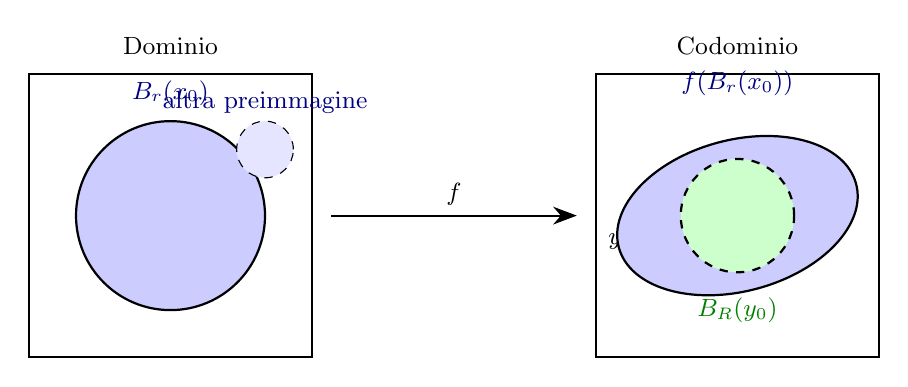
\begin{tikzpicture}[scale=1.2, every node/.style={font=\small}]

% Domini
\draw[thick] (0,0) rectangle (3,3);
\node at (1.5,3.3) {Dominio};

\draw[thick] (6,0) rectangle (9,3);
\node at (7.5,3.3) {Codominio};

% Punti centrali
\fill (1.5,1.5) circle (1pt) node[below left] {$x_0$};
\fill (7.5,1.5) circle (1pt) node[below left] {$y_0=f(x_0)$};

% Bolla nel dominio
\draw[fill=blue!20, thick] (1.5,1.5) circle (1);
\node[blue!50!black] at (1.5,1.5+1.3) {$B_r(x_0)$};

% Immagine deformata nel codominio
\begin{scope}
\clip (6,0) rectangle (9,3);
\draw[fill=blue!20, thick, rotate around={15:(7.5,1.5)}]
  (7.5,1.5) ellipse (1.3 and 0.8);
\end{scope}
\node[blue!50!black] at (7.5,2.9) {$f(B_r(x_0))$};

% Piccola bolla contenuta
\draw[fill=green!20, thick, dashed] (7.5,1.5) circle (0.6);
\node[green!50!black] at (7.5,0.5) {$B_R(y_0)$};

% Freccia fra i due spazi
\draw[-{Stealth[length=3mm]}, thick] (3.2,1.5) -- (5.8,1.5)
  node[midway, above] {$f$};

% Piccola indicazione di possibile preimmagine fuori
\draw[fill=blue!10, dashed] (2.5,2.2) circle (0.3);
\node[blue!50!black] at (2.5,2.7) {altra preimmagine};
\end{tikzpicture}
\end{center}

\stheorem{Teorema della funzione inversa}{
    Sia \(f \colon \Omega \subseteq \realnumbers^n \fromto \realnumbers^n\),
    \(\Omega\) aperto e sia \(x_0 \in \Omega\), e \(y_0 = f(x_0)\).
    Inoltre, \(\text{d}f(x_0) \in \text{GL}(\realnumbers^n)\).
    Allora, esiste un intorno \(U\) di \(x_0\) e \(V\) intorno di \(y_0\)
    aperti tali che \(f \colon U \fromto V\)
    è un diffeomorfismo.
}

\sexample{Diffeomorfismo locale non implica diffeomorfismo globale}{
    Sia \(f(x,y) = e^x(\cos y, \sin y)\) definita su \(\realnumbers^2\).
    È un diffeomorfismo locale? Basta verificare che
    il differenziale sia invertibile.
    \[
        \begin{pmatrix}
            e^x \cos y & -e^x \sin y \\
            e^x \sin y & e^x \cos y
        \end{pmatrix}
    \]
    Il determinante è sempre positivo, quindi è sempre infertibile.
    Quindi, \(f\) ha un diffeomorfismo locale.
    Tuttavia, la funzione non è iniettiva, in quanto è per esempio periodica,
    quindi non è invertibile e non vi è diffeomorfismo globale.
    (Cosa che invece funziona con le funzioni reali di una variabile)
}

\scorollary{}{
    Sia \(\Omega \subseteq \realnumbers^n\) aperto,
    \(f \colon \Omega \fromto \realnumbers^n\) tale che \(f \in \mathcal{C}^1(\Omega, \realnumbers^n)\),
    \(\text{d}f(x) \in \text{GL}(\realnumbers^n)\) per ogni \(x\in \Omega\).
    Allora, \(f(\Omega)\) è aperto.
}

\sproof{}{
    Sia \(y_0 \in f(\Omega)\).
    Vogliamo mostrare che \(y_0\) è introno di \(f(\Omega)\).
    Per definizione \(\exists x_0 \in \Omega\) tale che \(y_0 = f(x_0)\)
    e per ipotesi il differenziabile in quel punto è invertibile.
    Per il teorema della funzione inversa esistono quindi
    intorni \(U\) di \(x_0\) e \(V\) di \(y_0\) aperti
    tale che la funzione rispettra \(f \colon U \fromto V\) è un diffeomorfismo.
    In particolare, \(y_0 \in V = f(U) \subseteq f(\Omega)\).
    Quindi sono tutti punti interni.
}

In particolare, se \(\text{d}f(x) \in \text{GL}(\realnumbers^n)\)
per tutte le \(x \in \Omega\), allora \(f\) è una mappa aperta.
Infatti a volte questo si chiama teorema della mappa aperta.

Come detto, in una funzione di una variabile l'invertibilità della derivata è sufficiente
per l'invertibilità, mentre in molteplici variabili l'invertibilità del differenziale
mi garantisce solo l'invertibilità locale.
Possiamo aggiungere la condizione di inietività per garantire l'invertibilità globale.

\scorollary{}{
    Sia \(\Omega \subseteq \realnumbers^n\) aperto,
    \(f \colon \Omega \fromto \realnumbers^n\) tale che \(f \in \mathcal{C}^1(\Omega, \realnumbers^n)\),
    \(\text{d}f(x) \in \text{GL}(\realnumbers^n)\) per ogni \(x\in \Omega\)
    e \(f\) iniettiva in \(\Omega\).
    Allora, \(f^{-1} \in \mathcal{C}^1(f(\Omega), \realnumbers^n)\)
    e \(f \colon \Omega \fromto f(\Omega)\) è un diffeomorfismo.
}

\sproof{}{
    L'iniettività garantisce l'esistenza di
    \(f^{-1} \colon f(\Omega) \fromto \Omega\) e \(f(\Omega)\) è aperto.
    Sia \(y_0 = f(x_0) \in f(\Omega)\).
    Per il teorema della funzione inversa \(\exists r, R>0\)
    tali che \(f\colon f^{-1}(B_R(y_0)) \cap B_r(x_0) \fromto B_r(y_0)\)
    è un diffeomorfismo.
    In particolare, l'inverso di questa funzione è differenzuiabile.
    Ma essendo \(f\) iniettiva, questa inversa locale deve coincidere con l'inversa globale,
    e quindi \(f^{-1} \colon f(\Omega) \fromto \Omega\) è differenziabile.
}

\subsection{Trasformazioni di coordinate}

\begin{radioactive}
Le trasformazioni di coordinate mediante mappe affini sono diffeomorfismi.
Tuttavia, non tutte le trasformazioni, come per esempio le coordinate polari, sono affinità.
Queste trasformazioni devono essere biunivoche.
Per esempio le coordinate polari vanno ristrette a \(\theta\in(0,2\pi]\)
e \(\rho \neq 0\). Per riacquistare la suriettività dobbiamo togliere l'origine dal codominio.

\sdefinition{Trasformazione di coordinate}{
    Una trasformazione di coordinate di \(\realnumbers^n\)
    è un diffeomorfismo globale il cui dominio deve essere un insieme "grosso".
}
\end{radioactive}

\(f(\rho, \theta) = (\rho\cos\theta,\rho\sin\theta)\) è differenziabile,
ma l'inversa non è continua. Infatti il seguente limite non esiste (considerando \(\theta \in (-\pi, \pi]\))
\[
    \lim_{(x,y) \fromto (-1,0)} f^{-1}(x,y)
\]
possiamo considerare i due cammini circolari dal sopra e dal sotto.
Per rendere \(f\) un omeomorfismo, consideriamo
\(f \colon (0, +\infty) \times (-\pi, \pi) \fromto \realnumbers^2 \difference \{(x,0) \suchthat x \leq 0\}\).
\\
\begin{radioactive}
Inoltre abbiamo
\[
    \jacobian_f(\rho,\theta) = \begin{pmatrix}
        \cos\theta & -\rho\sin\theta \\
        \sin\theta & \rho\cos\theta
    \end{pmatrix}
\]
che ha determinante \(\rho>0\).
Per le coordinate cilindriche consideriamo
\[
    f\colon (0,+\infty) \times (-\pi, \pi)
    \times \realnumbers \fromto \realnumbers^3 \difference \{(x, 0, z) \suchthat x \leq 0\}
\]
la funzione è biiettiva inquesto dominio e inoltre
\[
    \jacobian_f(\rho,\theta, z) = \begin{pmatrix}
        \cos\theta & -\rho\sin\theta & 0 \\
        \sin\theta & \rho\cos\theta & 0 \\
        0 & 0 & 1
    \end{pmatrix}
\]
il cui determinante è il medesimo.
Quindi è anch'essa un diffeomorfismo globale.
Per le coordinate sferiche \((x,y,z) \to (\rho, \varphi, \theta)\) ho
\[
    f(\rho,\varphi,\theta) = (\rho\sin\varphi\cos\theta, \rho\sin\varphi\sin\theta,\rho\cos\varphi)
\]
con definizione
\[
    f\colon (0,+\infty) \times (0, \pi) \times (-\pi, \pi)
    \fromto
    \realnumbers^3 \difference \{(x,0,z) \suchthat x \leq 0\}
\]
Il Jacobiano è dato da
\[
    \jacobian_f(\rho,\varphi,\theta) = \begin{pmatrix}
        \sin\varphi\cos\theta & \rho\cos\varphi\cos\theta & -\rho\sin\varphi\sin\theta \\
        \sin\varphi\sin\theta & \rho\cos\varphi\sin\theta & \rho\sin\varphi\cos\theta \\
        \cos\theta & -\rho\sin\varphi & 0
    \end{pmatrix}
\]
il cui determinante è \(\rho^2 \sin\varphi > 0\).
\end{radioactive}

\pagebreak

\section{Estremi vincolati}

Notiamo che in generale, siccome il gradiente punta nella direzione di massima crescita, dobbiamo
studiare i punti in cui la direzione del gradiente della funzione è ortogonale
alla retta tangente del vincolo (esempio con cerchio unitario e piano \(x+y\)).
Per trovare lo spazio tangente al vincolo usiamo il teorema della funzione implicita
(perché magari non abbiamo la funzione direttamente).

\sexample{}{
    Consideriamo come varietà \(M = \Phi^{-1}(0)\)
    dove \(\Phi \colon \realnumbers^n \fromto \realnumbers^m\)
    con \(m < n\). Ho \(m\) equazioni in \(n\) incognite
    \(\Phi = (\Phi_1, \cdots, \Phi_m)\).
    Se tutto va bene, dato il sistema dei \(\Phi_i(x) = 0\),
    possiamo isolare \(m\) incognite in funzione delle altre \(m-n\).
    Sia \(k = m-n\) la dimensione di \(M\) (se tutto va bene)
    come varietà. \\
    Sia \(x_0 \in M\), \(\text{d}\Phi(x_0) \colon \realnumbers^n \fromto \realnumbers^m\).
    \(\jacobian_\Phi(x_0)\) è una matrice di tipo \(m\times n = (n-k)\times n\).
    Possiamo applicare il teorema della funzione implica se e solo se
    \(\jacobian_\Phi(x_0)\) è massi,o cioè \(\text{rank} \jacobian_\Phi(x_0) = n-k\), ovvero se
    \(\text{d}\Phi(x_0)\) è suriettivo. In questo caso, a meno di permutare le variabili posso scrivere
    \(x\in\realnumbers^n\) con \(x=(z,y)\) con \(z\in\realnumbers^n\) e \(y\in\realnumbers^{n-k}\) e
    \(\Phi_y(x_0) \in \text{GL}(\realnumbers^{n-k})\).
    \(M\) in un intorno di \(x_0\) può essere scritta nel modo seguente
    \((z,y) \in M\) se e solo se \(y = \varphi(z)\) dove \(\varphi\) è la funzione implicita.
    Se \(\Phi\) è di classe \(\mathcal{C}^1\), lo è pure \(\varphi\), quindi possiamo sviluppar
    \(\varphi\) al primo ordine
    \[
        y-y_0 = \text{d}\varphi(z_0)(z-z_0) + o(||z-z_0||)
    \]
    Ottengo lo spazio tangente trascurando l'o-piccolo e traslando nell'origine
    \[T_{x_0}M = \{(v,w) \in \realnumbers^k \times \realnumbers^{m-n} \suchthat w = \text{d}\varphi(z_0) v\}
    = \{(v, \text{d}\varphi(z_0)v)\}\]
}

\stheorem{}{
    Sia \(\Phi \colon \Omega \subseteq \realnumbers^n \fromto \realnumbers^{n-k}\),
    \(\Phi \in \mathcal{C}'(\Omega)\), \(x_0 \in \Omega\) tale che
    \(\Phi(x_0) = 0\), \(\text{d}\Phi(x_0)\) suriettivo.
    Sia \(M = \Phi^{-1}(0)\).
    Allora, \(T_{x_0}M = \text{ker} \,\text{d}\Phi(x_0)\).
}

\sproof{}{
    Sappiamo che \(\text{d}\varphi(z_0) = -\Phi_y(x_0)^{-1} \circ \Phi_y(x_0)\).
    \(w = \text{d}\varphi(z_0)v\) se e solo se \(\Phi_y(x_0) w = -\Phi_z(x_0)v\)
    se e solo se \(\Phi_z(x_0)v + \Phi_y(x_0)w = 0\) se e solo se
    \(\text{d}\phi(x_0)(v,w) =0\) se e solo se \((v,w) \in \text{ker} \,\text{d}\Phi(x_0)\). 
}

\sdefinition{}{
    Se \(M = \Phi^{-1}(0)\), \(\Phi(x) = 0\) e \(\text{d}\Phi(x_0)\) è surettiva, allora
    \(x_0\) è un punto regolare di \(M\).
}

\sexample{}{
    Sia \(M=S^1\), quindi \(\Phi(x,y) = x^2 + y^2 - 1\),
    \(M\Phi^{-1}(0)\). Dobbiamo calcolare il kernel di \(\text{d} \Phi(x_0, y_0)\).
    \[
        \text{d}\Phi(x_0, y_0)(v,w) = \nabla \Phi(x_0, y_0)(v,w) =0
        \implies
        T(x_0, y_0)M = \nabla \Phi(x_0, y_0) = (2x_0, 2y_0)
    \]
    Abbiamo che
    \[
        \nabla \Phi(x_0, y_0) = (0,0) \iff (x_0, y_0) = (0,0)
    \]
    ma \((0,0) \notin M\), quindi \(S^1\) è regolare.
    \[
        T_{(x,y,z)}S^1 = \{(v,w) \suchthat (x_0, y_0)(v,w) = 0\}
        = \{
            x_0v +y_0w = 0
        \} = \{(\lambda y_0 - \lambda x_0) \suchthat \lambda \in \realnumbers\}
        = \langle(y_0, x_0)\rangle
    \]
}

\sexample{}{
    Sia \(\Phi \colon \realnumbers^n \fromto \realnumbers\), \(M = \Phi^{-1}(0)\).
    \(\text{d}\Phi(x_0)v = \nabla \Phi(x_0)v = 0\)
    se e solo se \(v \perp \nabla \Phi(x_0)\).
    \(T_{x_0}M = \nabla \Phi(x_0)^\perp\).
    Lo spazio tangente agli insiemi di livello di \(\Phi\) e lo spazio ortogonale a \(\nabla \Phi(x_0)\)
    (se è non nullo, cioè se \(x\) è un punto regolare).
}

\sexample{}{
    Sia \(\Phi(x,y,z) = xyz^2 + 1\), \(M = \Phi^{-1}(0)\).
    Esistono punti \((x,y,z)\) di \(M\) tale che \((1,1,0) \in T_{(x,y,z)}M\) e
    \((0,1,1)\in T_{(x,y,z)}M\)?
    \(\nabla \Phi(x,y,z) = (yz^2,xz^2, 2xyz)\). Se si annulla almeno una delle tre corodinate 
    deve annullarsi \(\implies (x,y,z) \notin M\) perché \(\Phi(x,y,z) = 01\) e quindi \(M\) è regolare.
    Devo quindi imporre che \(\Phi(x,y,z) = 0\), che \(\nabla \Phi(x,y,z)(1,1,0) = 0\) e che
    \(\nabla \Phi(x,y,z)(0,1,1) = 0\).
    \begin{align*}
        \begin{cases}
            xyz^2 + 1 = 0\\
            yz^2 + xz^2 = 0\\
            xz^2 + 2xyz = 0
        \end{cases}
        \to
        \begin{cases}
            xyz^2 + 1 = 0 \\
            z^2(y + x) = 0 \\
            xz(z + 2y) = 0
        \end{cases}
        \to
        \begin{cases}
            x = -y \\
            z = -2y \\
            -4y^2 + 1 = 0
        \end{cases}
    \end{align*}
    quindi \(P \equiv (1 / \sqrt{2}, -1/\sqrt{2}, -\sqrt{2})\) e \(Q \equiv (-1/\sqrt{2}, 1/\sqrt{2}, -\sqrt{2})\).
    Siccome \(\text{dim} T \times M = 2\) implica \(TpM = \langle(1,1,0),(0,1,1)\rangle = T_aM\).
    Consideriamo il caso generale \(\Phi \colon \Omega \subseteq \realnumbers^n \fromto \realnumbers^{n-k}\).
    \(M = \Phi^{-1}(0)\). Ci aspettiamo che, se \(x_0\) è un punto regolare,
    che \(M\) sia \(k\)-dimensionale (per lo meno in un intorno di \(x_0\))
    \[
        M = \begin{cases}
            \Phi_1(x) = 0\\
            \Phi_{n-k}(x) = 0
        \end{cases}
    \]
    vogliamo caratterizzare \(T_{x_0} M = \text{ker}\,\text{d}\Phi(x_0)\).
    Vale \(\text{d}\Phi(x_0)v = 0\) se e solo se \(J \Phi(x_0)v = 0\) se e solo se
    \[
        \begin{pmatrix}
            \nabla \Phi_1(x_0)_\perp \\
            \vdots \\
            \nabla \Phi_{n-k}(x_0)_\perp
        \end{pmatrix} v = 0 \iff
        \begin{pmatrix}
            \nabla \Phi_1(x_0) \cdot v \\
            \vdots \\
            \nabla \Phi_{n-k}(x_0) \cdot v
        \end{pmatrix} = \begin{pmatrix}
            0 \\ \vdots \\ 0
        \end{pmatrix}
    \]
    meaning that \(v\in T_{x_0}M\) if and only if \(v_1 \nabla \Phi_i(x_0) = 0\).
    Cioè, \(T_{x_0}M^\perp = \langle \nabla \Phi_1(x_0), \cdots, \nabla \Phi_{n-k}(x_0)\rangle\)
    ovvero \(T_{x_0}M = \langle \nabla \Phi_1(x_), \cdots, \nabla \Phi_{n-k}(x_0) \rangle^\perp\)
    e \(\nabla \Phi_1(x_0), \cdots, \nabla \Phi_{n-k}(x_0)\) sono l.i. perché i triangoli
    delle righe di \(\jacobian_\Phi(x_0)\) e per ipotesi \(\jacobian_\Phi(x_0) = \text{rank} n-k\).
}

\sexample{}{
    Sia
    \[
        \Phi(x,y,z) = \begin{pmatrix}
            x + y^2 + 3z \\ xz + y^2
        \end{pmatrix}
    \]
    \(\phi \colon \realnumbers^3 \fromto \realnumbers^2\).
    Posto \(M = \Phi^{-1}(0,0)\), trovare \(T_{(0,0,0)}M\).
    \[
        \jacobian_\Phi = \begin{pmatrix}
            1 & 2y & 3 \\ z & 2y & x
        \end{pmatrix}, \quad \jacobian_\Phi(0,0,0) = \begin{pmatrix}
            1 & 0 & 3 \\ 0 & 0 & 0
        \end{pmatrix}
    \]
    \(\text{rank} \jacobian_\Phi(0,0,0) = 1\), quindi non è massimo.
    \(\text{dim}\,\text{ker}\,\text{d}\Phi(0,0,0) =2\), ma \(k=1\).
    Il problema è che il punto non è regolare.
}

\sexample{}{
    Sia \(\Phi\colon \realnumbers^4 \fromto \realnumbers^2\) e \(M = \Phi^{-1}(0)\).
    Supponiamo che \(0\in M\), cioè che \(\Phi(0)=0\) e che
    \[
        \jacobian_\Phi(0) = \begin{pmatrix}
            -1 & 1 & 0 & 1 \\ 2 & 0 & 1 & -1
        \end{pmatrix}
    \]
    Determinare \(T_0 M\). Abbiamo \(\text{rank} \, \text{d} \Phi(0)=2\) è massimo,
    e quindi \(0\) è un punto regolare di \(M\).
    \[
        \left(T_0M\right)^\perp = \langle \begin{pmatrix}
            -1 \\ 1 \\ 0 \\ 1
        \end{pmatrix}, \begin{pmatrix}
            2 \\ 0 \\ 1 \\ -1
        \end{pmatrix}
        \rangle = \left\{
            \lambda \begin{pmatrix}
                -1 \\ 1 \\ 0 \\ 1
            \end{pmatrix}
            + \mu \begin{pmatrix}
                2 \\ 0 \\ 1 \\ -1
            \end{pmatrix}
            \suchthat \mu, \lambda \in \realnumbers
        \right\}
    \]
    Sia \((x,y,z,w) \in \realnumbers^4\). Devo imporre l'ortogonalità alle righe della matrice
    \(\jacobian_\Phi(0)\)
    \[
        \begin{cases}
            -x + y + w = 0 \\
            2x + z - w = 0
        \end{cases}
    \]
    Risolviamo \(z,w\) in funzione di \(x,y\).
    \begin{align*}
        \begin{pmatrix}
            -1 & 1 \\ 2 & 0
        \end{pmatrix}
        \begin{pmatrix}
            x \\ y
        \end{pmatrix}
        + \begin{pmatrix}
            0 & 1 \\ 1 & -1
        \end{pmatrix}
        \begin{pmatrix}
            z \\ w
        \end{pmatrix} = \begin{pmatrix}
            0 \\ 0
        \end{pmatrix} \\
        \begin{pmatrix}
            z \\ w
        \end{pmatrix} = {-\begin{pmatrix}
            0 & 1 \\ 1 & -1
        \end{pmatrix}}^{-1}
        \begin{pmatrix}
            -1 & 1 \\ 2 & 0
        \end{pmatrix}
        \begin{pmatrix}
            x \\ y
        \end{pmatrix} = \cdots = \begin{pmatrix}
            -1 & -1 \\ 1 & -1
        \end{pmatrix}
        \begin{pmatrix}
            x \\ y
        \end{pmatrix}
    \end{align*}
    e
    \[
        T_0 M = \left\{
            \begin{pmatrix}
                x \\ y \\ -x-y \\ -x-y
            \end{pmatrix} \suchthat x,y \in \realnumbers
        \right\} = \langle \begin{pmatrix}
            1 \\ 0 \\ -1 \\ 1
        \end{pmatrix}, \begin{pmatrix}
            0 \\ 1 \\ -1 \\ -1
        \end{pmatrix} \rangle
    \]
}

\sdefinition{}{
    \(M \subseteq \realnumbers^m\) è una sottovarietà \(k\)-dimensionale
    se \(\forall x_0 \in M\), esiste \(V \subseteq \realnumbers^m\) aperto, \(x_0 \in V\)
    ed esiste \(\Phi \in \mathcal{C}^1(V, \realnumbers^{n-k})\) tale che
    \(M \intersection V = \Phi^{-1}(0)\) e \(\text{d}\Phi(x_0)\) sia suriettivo.
}

Dato \(M\) sottovarietà \(k\)-dimensionale
di \(\realnumbers^n\), vorrei definire lo spazio tangente ad \(M\)
in \(x_0\) come \(\text{ker}\,\text{d}\Phi(x_0)\), dove \(\Phi\) è
una funzione definita in un intorno di \(x_0\) come nella definizione.
Il problema è che lo stesso \(M\) può essere descritto da molte \(\Phi\) diverse.

\sexample{}{
    Sia \(M = \{(x,y) \suchthat y=0\}\), \(\Phi(x,y) = y\).
    \(\Xi(x,y) = y(x^2 + 1)\), \(\Psi(x,y) = y(x^2 + y^2)\).
    \(\nabla \Phi = (0,1)\), quindi \((0,0)\) è un punto regolare per questo \(\Phi\).
    \(\nabla \Psi = (2xy, 3y^2)\), \((0,0)\) non è un punto regolare.
}

\sdefinition{}{
    Sia \(M \subseteq \realnumbers^n\) una sottovarietà \(k\)-dimensionale
    se \(\forall x_0 \in M\) esiste un intorno di \(x_0\) e una funzione
    \(\varphi \colon \realnumbers^k \fromto \realnumbers^{n-k}\) (di cui le variaibli
    le chiamiamo \(x\) e \(y\)) tale che \((z,y) \in M\) se e solo se \(y = \varphi(z)\)
    (a mano di permutazioni delle variabili).
}

Le due definizioni sono equivalenti:
sia \(\Phi\) tale che \(M = \Phi^{-1}(0)\) nell'intorno di \(x_0\) e
\(\text{d}\Phi(x_0)\) sia suriettivo.
Allora per il teorema della funzione implicita esiste la \(\varphi\) della seconda definizione.
Viceversa, se \(\varphi\colon \realnumbers^k \fromto \realnumbers^{n-k}\) definisce
\(M\) localmente, basta scegliere \(\Phi(z,y) = y-\varphi(z)\) e la funzione \(\Phi\) soddisfa
la definizione precedente di sottovarietà.
Vogliamo dare una definizione dello spazio tangente che sia indipendente dalla scelta
di \(\Phi\). Consideriamo un cammino \(\gamma\) sulla sottovarietà \(M\), cioè un'applicazione
derivabile \(\gamma \colon (-\varepsilon, \varepsilon) \fromto M\) tale che \(\gamma(0) = x_0\).
\(\dot{\gamma}(0)\) è un vettore in \(\realnumbers^n\) ed è tangente al supporto di \(\gamma\) in \(x_0\).
Facendo varriare il cammino otteniamo tutti e soli i vettori tangenti
ad \(M\) in \(x_0\), cioè \[
    T_{x_0}M = \{
        \dot{\gamma}(0) \suchthat \gamma \colon (-\varepsilon, \varepsilon) \fromto M
        \text{ cammino } \suchthat \gamma(0) = x_0
    \}
\]
Vogliamo dimostrare che questa definizione di spazio tangente coincide con quelle vecchie,
cioè con \(\text{ker}\,\text{d}\Phi(x_0)\) dove \(\Phi^{-1}(0) = M \intersection V\).
Poniamo
\[
    X = \{
        \dot{\gamma} \suchthat \gamma \colon (-\varepsilon, \varepsilon) \fromto M
        \text{ cammino } \land \gamma(0) = x_0
    \}
\]
Sia \(x \in X\), cioè \(v = \dot{\gamma}(0)\) con \(\gamma \colon (-\varepsilon, \varepsilon) \fromto M\)
cammino tale che \(\gamma(0) = x_0\) e sia
\(\Phi \in \mathcal{C}^1(\mathcal{U}(x_0), \realnumbers^{n-k})\) tale che
\(M \intersection \mathcal{U}(x_0) = \Phi^{-1}(0)\) e \(\text{d}\Phi(x_0)\) sia suriettivo.
Verifichiamo che \(v \in \text{ker} \, \text{d}\Phi(x_0)\).
Consideriamo \(\Phi \circ \gamma \colon (-\varepsilon, \varepsilon) \fromto \realnumbers^{n-k}\) è la
funzione identicamente nulla perché per ipotesi \(\gamma\) è un cammino in \(M\), quindi
\(\gamma(t) \in M\) per tutte le \(t\), e allora \(\Phi(\gamma(t)) = 0\).
Calcoliamo \((\Phi\circ\gamma)'(0)\)
\[
    0 = (\Phi\circ\gamma)'(0) = \text{d}\Phi(\gamma(0))\dot{\gamma}(0) = \text{d}\Phi(x_0)v
    \implies v \in\text{ker}\,\text{d}\Phi(x_0)
\]
Dobbiamo dimostrare l'inclusione opposta, cioè che se \(v \in \text{ker}\,\text{d}\Phi(x_0)\) 
allora esiste \(\gamma \colon (-\varepsilon, \varepsilon) \fromto M\) tale che
\(\gamma(0) = x_0\) e \(\dot{\gamma}(0) = v\). Se non fossimo vincolati a stare in \(M\) potremmo
scegliere \(\gamma(t) = x_0 + tv\).
Vogliamo definire una curva \(\gamma \colon (-\varepsilon, \varepsilon) \fromto M\)
tale che \(\gamma(0) = x_0\) e \(\dot\gamma(0)=v\).
Siccome \(\text{d}\Phi(x_0)\) è suriettivo per ipotesi, possiamo applicare il teorema della
funziona implicita, esiste quindi locamente \(\varphi \colon \realnumbers^n \fromto \realnumbers^{n-k}\)
tale che \((z,y) \in M \intersection V\) se e solo se \(y = \varphi(z)\).
Cioè, localmente vicino ad \(x_0\), riesco a scrivere \(M\) come il grafico di una funzione di \(k\)
variabili (a meno di permutare le variabili).
Allora possiamo dividere \(v = (\alpha, \beta)\)
dove \(\alpha\) sono le prime \(k\) componenti e \(\beta\) sono le \(n-k\) componenti successive.
La condizione che \((\alpha,\beta) \in \text{ker}\,\text{d}\Phi(x_0)\), cioè chde sia vettore tangente, è che
\(\beta = \text{d}\varphi(x_0) \alpha\).
Per costruire la curva, per le prime \(k\) componenti scegliamo le rette, e di conseguenza
le altre componenti devono essere \(\varphi\) delle prime. Quindi definiamo
\[
    \gamma(t) = (z_0 + t\alpha, \varphi(z_0 + t\alpha)) \in M, \quad \forall t
\]
e inoltre \(\varphi(0) = (z_0, \varphi(z_0)) = (z_0, y_0) = x_0\).
Verifichiamo che sia effettivamente tangente, quindi calcoliamo la derivata usando la chain rule
\[
    \dot\gamma(t) = (\alpha, \text{d}\varphi(z_0 + t\alpha)\alpha)
\]
e per \(t=0\)
\[
    \dot\gamma(0) = (\alpha, \text{d}\varphi(z_0)\alpha) = (\alpha, \beta) = v
\]

\sexample{Sottovarietà}{
    La sfera unitaria è una sottovrietà \((n-1)\)-dimensionale di \(\realnumbers^n\)
    \[
        S^{n-1} = \{x\in \realnumbers^n \colon ||x|| = 1\}
    \]
}

\sexample{Sottovarietà}{
    Il cilindro è una sottovarietà in \(\realnumbers^3\).
    Abbiamo \(\Phi(x,y,z) = x^2 + y^2 - 1\) e \(\gradient \Phi(x,y,z) = (2x,2y,0)\).
    Quest'ultima si annulla nei punti dell'asse \(z\), ma \(\Phi(0,0,z) \neq 0\)
    e quindi tutte i punti sono regolari.
    Lo stesso vale per tutte le quadriche singolari (cono e quadriche che si spezzano, come piani che si intersecano)
}

\sexample{Toroid}{
    Il toro è una superficie regolare in \(\realnumbers^3\) in quanto si può scrivere
    come luogo di zeri.
    Il toro non può essere una quadrica in quanto una retta può intersecare un toro in al più di quattro punti,
    quindi è una superficie algebrica, cioè luogo degli zeri di di un poinomio di quarto grado.
    \begin{align*}
        (\sqrt{x^2 + y^2} - R)^2 + z^2 &= r^2 \\
        (x^2 + y^2 + z^2 + R^2 - r^2)^2 &= 4R^2(x^2 + y^2)
    \end{align*}
    e otteniamo una quartica.
}

Torniamo quindi agli estremi vincolati. Sia
\(f\colon \Omega \colon \realnumbers^n \fromto \realnumbers\).
Sia \(M \subseteq \realnumbers^n\) il vincolo, che supponiamo essere una sottovarietà
\(k\)-dimensionale di \(\realnumbers^n\).
Supponiamo \(f \in \mathcal{C}^1(\Omega)\).
Vogliamo ottimizzare \(\restr{f}{M}\).
\(f\) ha un massimo locale vincolato ad \(M\)
in \(x_0\) se \(\restr{f}{M}\) ha un massimo locale in \(x_0\), ovvero
se esiste un \(V\) aperto tale che \(x_0 \in V\) e \(f(x) \leq f(x_0)\)
per tutte le \(x\in V \intersection M\).

\stheorem{}{
    Sia \(f \colon \Omega \subseteq \realnumbers^n \fromto \realnumbers\)
    con \(\Omega\) aperto e \(f \in \mathcal{C}^1(\Omega)\).
    Sia \(M \subseteq \realnumbers^n\) il vincolo, che supponiamo essere una sottovarietà
    \(k\)-dimensionale di \(\realnumbers^n\).
    Sia \(x_0 \in M\) un punto di estremo locale per \(f\) vincolato ad \(M\).
    Allora, \(\gradient f(x_0) \cdot v = 0\)
    per tutte le \(v \in T_{x_0}M\).
}

Il teorema afferma che la condizione necessaria affinché \(x_0\)
sia punto di estremo vincolato
è che le derivate direzionali di \(f\) siano nulle in tutte le direzioni tangent al vincolo.

\sdefinition{Punto critico vincolato}{
    \(x_0\) è punto critico di \(f\) vincolato ad \(M\) se \(\gradient f(x_0) \cdot v = 0\)
    per tutte le \(v \in T_{x_0}M\).
}

Questi potrebbero quindi non essere estremanti, è solo una condizione necessaria.

\sproof{}{
    Usiamo la caratterizzazione dello spazio tangente con i cammini.
    Sia \(v \in T_{x_0} M\). Allora \(v = \dot\gamma(0)\)
    con \(\gamma \colon (-\varepsilon, \varepsilon) \fromto M\)
    e \(\gamma(0) = x_0\).
    Consideriamo \(f \circ \gamma\).
    Per ipotesi, \(f\) ha un punto estremante in \(x_0\) vincolato da \(M\),
    quindi anche \(f \circ \gamma\) ha un punto estremante in \(x_0\) siccome \(\gamma(t) \in M\)
    per tutte le \(t\).
    Abbiamo quindi una funzione reale di una variabile che ha un punto estremante in \(t=0\),
    ed è differenziabile, quindi \begin{align*}
        (f\circ\gamma)'(0) = \gradient f(\gamma(0)) \cdot \dot\gamma(0)
         = \gradient f(x_0) \cdot v = 0
    \end{align*}
    Dall'arbitrarietà segue la tesi.
}

Nel caso (degli esercizi) dove \(M=\Phi^{-1}(0)\)
con \(\Phi\colon \realnumbers^n \fromto \realnumbers^m\)
con \(m<n\) e \(\Phi \in \mathcal{C}^1(Omega, \realnumbers^m)\)
dato da \(\Phi = (\Phi_1, \cdots, \Phi_m)\).
In questo caso se \(x_0\) è un punto regolare di \(M\),
\(T_{x_0}M = \text{ker}\,\text{d}\Phi(x_0)\) e sappiamo che
\[
    {[\text{ker}\,\text{d}\Phi(x_0)]}^\perp = \langle 
        \gradient \Phi_1(x_0), \cdots,
        \gradient \Phi_m(x_0) \rangle
\]
\(x_0\) è puto critico vincolato su
\[
    \gradient f(x_0) \in
    {[\text{ker}\,\text{d}\Phi(x_0)]}^\perp = \langle 
        \gradient \Phi_1(x_0), \cdots,
        \gradient \Phi_m(x_0) \rangle
\]
Cioè \(x_0\) è punto critico vincolato su \(\gradient f(x_0)\) è combinazione lineare
di \(\gradient \Phi_1(x_0), \cdots, \gradient \Phi_n(x_0)\),
cioè esistono \(\lambda_i\) tali che
\[
    \gradient f(x_0) = \sum_i \lambda_i \gradient \Phi_i(x_0)
\]
Questo equivalente a risolvere \(m+n\) equazioni in \(m+n\) incognite,
cioè dobbiamo imporre che \(x\) stia nel vincolo e trovare sia gli \(x\) che i \(\lambda\)
\[
    \begin{cases}
        \gradient f(x_0) = \sum_i \lambda_i \gradient \Phi_i(x_0) \\
        \Phi_1(x) = 0 \\
        \vdots \\
        \Phi_m(x) = 0
    \end{cases}
\]

Possiamo quindi trovare i punti critici ma ci manca un criterio del secondo ordine
per determinare se sono punti estremanti e di che tipo.

\sexercise{}{
    Sia \(f(x,y) = xy\). Troviamo i punti critici di \(f\)
    vincolati a \(\Phi(x,y) = x^2 - xy + y^2 - 1 = 0\).
    Dobbiamo inizialmente verificare che il vincolo sia regolare.
    Il gradiente
    \[
        \gradient \Phi(x,y) = (2x-y,2y-x)
    \]
    che si annulla per
    \[
        \begin{cases}
            2x-y=0 \\
            2y-x =0
        \end{cases}
    \]
    siccome la matrice associata è non singolare, il gradiente si annulla se e soltanto se
    \((x,y)=(0,0)\). Ma questo punto non fa parte del vincolo \(\Phi(0,0) \neq 0\).
    Quindi, il vincolo è regolare.
    I piunti critici vincolari sono la soluzione del sistema
    \[
        \begin{cases}
            y = \lambda(2x-y) \\
            x = \lambda(2y-x) \\
            x^2 - xy + y^2 = 1
        \end{cases}
    \]
    Siccome le prime due sono lineari possiamo riscriverle come
    \[
        \begin{pmatrix}
            2\lambda & -1-\lambda \\
            1 + \lambda & -2\lambda
        \end{pmatrix}\begin{pmatrix}
            x \\ y
        \end{pmatrix}
        = \begin{pmatrix}
            0 \\ 0
        \end{pmatrix}
    \]
    L'unica speranza di avere un punto critico è che il determinante si annulli, quindi
    \begin{align*}
        -4\lambda^2 + {(1 + \lambda)}^2 &= \\
        (1 + \lambda + 2\lambda)(1 + \lambda - 2\lambda) &= 0 \\
        (3\lambda + 1) (1 - \lambda) &= 0
    \end{align*}
    Quindi serve \(\lambda = 1\) oppure \(\lambda = -1/3\).
    Cominciamo con \(\lambda = 1\),
    \[
        \begin{cases}
            \lambda = 1 \\
            y = 2x - y \\
            x^2 - xy + y^2 = 1
        \end{cases}
    \]
    da cui ricaviamo \(y=x\) e \(x^2\).
    Quindi i punti critici sono \(A = (1,1)\) e \(B = (-1, -1)\).
    Impostiamo ora \(\lambda = -1/3\), abbiamo 
    \[
        \begin{cases}
            \lambda = -\frac13 \\
            3y = 2x-y \\
            x^2 - xy + y^2 = 1
        \end{cases}
    \]
    da cui ricaviamo \(x = -y\)
    e \(x = \pm 1 / \sqrt{3}\).
    Quindi otteniamo i punti critici \(C = (1 / \sqrt{3}, -1 / \sqrt{3})\)
    e \(D = (-1/\sqrt{3}, 1/ \sqrt{3})\).
    Abbiamo \(f(A) = f(B) = 1\) e \(f(C) = f(D) = -1/3\).
    Se il vincolo è compatto, quindi per Weierstrass sappiamo che c'è un massimo e un minimo
    assoluto, e quindi è ovvio quali siano quali.
    Il vincolo è chiuso in quanto è \(\Phi^{-1}(0)\) con \(\Phi\) continua (preimmagine di un chiuso è chiuso su funzione continua).
    Per mostrare che il vincolo è limitato studiamo il limite
    \begin{align*}
        \lim_{(x,y) \fromto \infty} \Phi(x,y)
    \end{align*}
    Supponiamo che il limite sia per esempio \(7\),
    quindi esiste \(\varepsilon > 0\) tale che esiste \(R>0\)
    tale che per \(||x||>R\), \(|\Phi(x,y) - 7| < \varepsilon\), e quindi
    in particolare i valori di \(\Phi\) sono diversi da zero fuori da tale bolla, e quindi la
    \(\Phi\) si può annullare solamente nella bolla di raggio \(R\), ed è quindi limitato.
    Per il limite prendiamo come candidato la curva \(\Phi(x,0) = x^2 - 1 \to \infty\).
    Calcoliamo il limite con delle stime e lo minoriamo con qualcosa che tende a infinito
    \begin{align*}
        \lim_{(x,y) \fromto \infty} \Phi(x,y)
        &= \lim_{(x,y) \fromto \infty} x^2 - xy + y^2 - 1 \\
        &\geq \lim_{(x,y) \fromto \infty} x^2 - \frac{x^2 + y^2}{2} + y^2 - 1 \\
        &= \frac{1}{2}(x^2 + y^2)- 1 \to \infty
    \end{align*}
    Se lo facessimo in coordinate polari possiamo usare il fatto che \(\sin\theta\cos\theta \leq 1/2\).
}

\sexercise{}{
    Trovare i punti di minima distanza dall'origine
    della curva \(x^2y = 1\).
    Dobbiamo massimizzare la funzione della distanza
    dall'origine, quindi \(f(x,y) = \sqrt{x^2 + y^2}\).
    Buttiamo via la radice per semplicità.
    Il vicolo è quindi \(\Phi = x^2 y - 1 = 0\).
    Possiamo parametrizzare il vincolo come grafico di funzione
    \(y = 1 / x^2\). Allora dobbiamo massimizzare la funzione \(g(x) = f(x, 1/x^2) = x^2 + 1/x^4\).
    (oppure \(y^2 + 1/y\)). Facciamolo con i moltiplicatori di Lagrange
    come esercizio. Assicuriamoci che il vincolo sia regolare, quindi il gradiente
    \(\gradient \Phi= (2xy, x^2) = (0,0)\) se e solo se siamo nei punti della forma \((0,y)\),
    che però non fanno parte del vincolo. Quindi, il vincolo è regolare.
    Dobbiamo quindi risolvere
    \[
        \begin{cases}
            2x = 2\lambda xy \\
            2y = \lambda x^2 \\
            x^2y = 1
        \end{cases}
    \]
    Otteniamo i casi \(x=0\) e \(\lambda y = 1\).
    Nel primo caso le tre equazioni non sono soddisfatte in contemporanea,
    ma nell'altro caso otteniamo i punti
    \((\pm \sqrt[6]{2}, 1 / \sqrt[3]{2})\) e \(\lambda = \sqrt[3]{2}\).
    Il vincolo è illimitato quindi non possiamo applicare Weierstrass,
    e quindi non possiamo garantire facilmente se c'è un minimo.
    Chiaramente \(f\) in questi punti coincide ed è positivo.
    Per risolvere questo problema consideriamo una bolla di raggio \(R\)
    sufficiente grande, e provare che la funzione sul bordo della bolla assume valori grandi.
    Visto che la funzione è la distanza, il valore sul bordo è sempre \(R^2\) che tende ad infinito,
    quindi il minimo avviene all'interno della bolla.
}

\sexercise{}{
    Fra tutti i parallelepipedi di superficie finita, dimostrare che il cubo è quello di volume massimo.
    Abbiano \(V(x,y,z) = xyz\) e la superficie è \(S = 2xy +2xz + 2yz > 0\).
    Abbiamo \(\Phi(x,y,z) = xy + xz + yz - S/2\).
    Verifichiamo che il vincolo sia regolare.
    \(\gradient \Phi(x,y,z) = (y + z, x + z, x + y) = (0,0,0)\)
    se e solo se \(x=y=z=0\), quindi è regolare. Si potrebbe pure esplicitare il vincolo
    ma usiamo i moltiplicatori di Lagrange.
    Abbiamo \(\gradient V = (yz, xz, xy) = \lambda \gradient \Phi\). Il sistema è
    \[
        \begin{cases}
            yz = \lambda (y + z) \\
            xz = \lambda (x + z) \\
            xy = \lambda (x + y) \\
            xy + xz + yz = \frac{S}{2}
        \end{cases}
    \]
    Deve essere \(\lambda,x,y,z \neq 0\). Se fosse \(\lambda =0\) avremmo \(S=0\) che è assurdo.
    Se una variabile si annulla, tutte le altre due si annulla e ciò non è possibile nel vincolo.
    Moltiplichiamo la prima equazione per \(x\) e la seconda per \(y\),
    quindi \(xyz = \lambda(xy + xz) = \lambda(xy + yz)\).
    Quindi, \(xy + xz = xy + yz\) cioè \(xz = yz\) cioè \(x=y\).
    Per simmetria, facedo la stessa cosa sulla terza equazione otteniamo \(x=z\).
    Quindi \(x=y=z\) che è il cubo.
    Per trovare il valore del lato sfruttiamo l'ultima equazione,
    quindi \(x = \sqrt{5/6}\) da cui possiamo trovare il volume.
    Dobbiamo mostrare che ciò è un massimo.
    Possiamo pure prendere \(x,y,z \geq 0\) in quanto se ci troviamo sui piani
    coordinati il paralellepipedo è degenere, e non è massimo sicuramente.
    Quindi, il vincolo è chiuso in quanto preimmagine di \(0\).
    Tuttavia, il vincolo non è limitato in quanto \(xy + xz + yz = S/2\)
    (è un iperbolide ellittico) e una sua sezione è un iperbole quindi è illimitata.
    Per esempio sezionando con il piano \(z=0\).
    Non possiamo quindi usare il teorema di Weierstrass.
    Consideriamo quindi l'intersezione del vincolo con una bolla chiusa
    di raggio \(\sqrt{3}\). Scegliamo questo raggio per semplicità per i prossimi conti,
    quindi \(x^2 + y^2 z^2 \leq 3R^2\).
    Considerando \(R\) sufficientemente grande, siamo su un compatto
    e che quindi amemtte massimo. Il massimo si può trovare o all'interno
    o sul bordo. Dobbiamo escludere che si trovi sul bordo.
    Guardiamo quanto fa il volume sul bordo della bolla, e mostriamo che tende a zero
    \[
        \restr{V}{\partial \overline{B}_{\sqrt{3}R}} \to 0
    \]
    Sulla frontiera della bolla \(x^2 + y^2 + z^2 = 3R^2\), quindi almeno uno dei tre quadrati
    deve essere maggiore di \(R^2\) (il motivo per cui abbiamo scelto quel coefficiente).
    Scegliamo senza perdita di generalità \(x^2 \geq R^2\).
    Siccome \(xz + yz + xy = S/2\) deve essere \(xz \leq S/2\) e \(xy \leq S/2\) e quindi
    \(z \leq S/(2x)\) e \(y\leq S/(2x)\). Il volume è dato da
    \[
        V(x,y,z) = xyz \leq x \frac{S}{2x} \frac{S}{2x}
        = \frac{S^2}{4x} \leq \frac{S^2}{4R} \to 0
    \]
    per \(R \to \infty\).
}

\sexercise{}{
    Vogliamo determinare gli estremi di \(f(x,y,z) = x^2 - x + y^2 + y(z + x - 1)\)
    vincolato da
    \[
        \begin{cases}
            x^2 + y^2 = 1 \\
            x + y + z = 1
        \end{cases}
    \]
    Anche in questo caso è possibile parametrizzare il vincolo ma lo facciamo con i
    moltiplicatore di Lagrange.
    Verifichiamo che il vincolo è determinare. Il vincolo è determinato da
    \[
        \Phi(x,y,z) = \begin{pmatrix}
            x^2 + y^2 - 1 \\
            x + y + z - 1
        \end{pmatrix}
    \]
    Per verificare che sia regolare verifichiamo che la Jacobiana abbia rango massimo, cioè \(2\)
    \[
        \jacobian_\Phi(x,y,z) = \begin{pmatrix}
            2x & 2y & 0 \\
            1 & 1 & 1
        \end{pmatrix}
    \]
    Notiamo che abbiamo un minore \(2\times 2\) sulla destra che si annulla
    se e solo se \(y=0\), mentre se prendiamo il minore con la prima colonna e  terza colonna,
    si annulla se e solo se \(x=0\).
    Quindi il rango è minore di due se e solo se \(x=y=0\).
    Ma se \(x=y=0\) allora la prima equazione non è soffisfatta, quindi il vincolo è regolare.
    Il gradiente è dato da \(\gradient f(x,y,z) = (2x + y - 1, 2y + z + x - 1, y)\).
    Il sistema è \(\gradient f = \lambda \gradient \Phi_1 + \mu \gradient \Phi_2\)
    \[
        \begin{cases}
            2x + y - 1 = \lambda 2x + \mu \\
            2y + z + x - 1 = \lambda 2y + \mu \\
            y = \lambda \cdot 0 + \mu \\
            x^2 + y^2 = 1 \\
            x + y + z = 1
        \end{cases}
    \]
    Dalla terza \(y=\mu\) e semplifichiamo
    \[
        \begin{cases}
            2x + y - 1 = \lambda 2x + y \\
            2y + z + x - 1 = \lambda 2y + y \\
            x^2 + y^2 = 1 \\
            x + y + z = 1
        \end{cases}
    \]
    Sostituiamo la quinta nella terza e ricaviamo \(2\lambda y = 0\),
    quindi o \(\lambda = 0\) oppure \(y = 0\). Supponendo \(\lambda = 0\)
    otteniamo \(x=\frac12\) e \(y = \pm \sqrt{3} /2\) e \(z = \frac12 \mp \sqrt{3} / 2\).
    Quindi abbiamo trovato i punti critici
    \[
        A \equiv \left(\frac12, \frac{\sqrt{3}}{2}, \frac{1 - \sqrt{3}}{2}\right), \quad
        B \equiv \left(\frac12, \frac{-\sqrt{3}}{2}, \frac{1 + \sqrt{3}}{2}\right), \quad
    \]
    Se invece supponiamo \(y=\mu = 0\) otteniamo \(x = \pm 1\),
    \(z = 1 - x\)
    \[
        \lambda = \frac{2x - 1}{2x} = \begin{cases}
            \frac12  \\
            \frac32
        \end{cases}
    \]
    quindi abbiamo anche i punti critici
     \[
        C \equiv \left(1, 0, 0\right), \quad
        D \equiv \left(-1, 0, 2\right), \quad
    \]
    Il vincolo è l'intersezione fra un cilindro ed un piano, quindi un'ellisse,
    quindi compatto. Per dire che è limitato potremmo dire \(|x|, |y| \leq 1\)
    e \(|z| \leq 1 + |x| + |y| \leq 3\). Chiaramente è chiuso
    in quanto preimmagine di di zero tramite funzione continua.
    Possiamo applicare Weierstrass. Abbiamo i seguenti punti
    \[
        f(A) = f(B) = -\frac14, \quad f(C) = 0, \quad f(D) = 2
    \]
    quindi \(A,B\) sono punti di minimo assoluto e \(D\) di massimo assoluto.
    Per l'altro punto serve un criterio del secondo ordine, per stabilirne la natura.
    Nel caso dell'ottimizzazione libera \(x_0\) era un punto critico se
    \(\text{d}f(x_0) v = 0\) per tutte le \(v \in \realnumbers^n\).
    Se \(x_0\) era critico, guardavamo il segno di \(\text{d}^2f(x_0)\) come applicazione
    bilineare
    \(\realnumbers^n \times \realnumbers^n \fromto \realnumbers\).
    Questo \(x_0\) è punto critico vincolato se \(\text{d}f(x_0) v = 0\)
    per tutti i \(v \in T_{x_0}M\).
    Come criterio del second'ordine dovremo stabilire il segno della forma bilineare
    \(\text{d}^2 f(x_0) - [\lambda_1 \text{d}^2 \Phi_1(x_0) + \cdots + \lambda_m \text{d}^2 \Phi_m(x_0)]\)
    sui vettoir di \(T_{x_0} M\).
    Dobbiamo quindi trovare lo spazio tangente al vincolo.
    In questo caso, il vincolo è una curva, quindi lo spazio tangente deve avere dimensione \(1\).
    Lo spazio tangente è lo spazio ortogonale allo generato dai gradienti di \(\Phi\)
    \[
        T_{x_0}M = \langle \gradient \Phi_1(x_0), \gradient \Phi_2(x_0) \rangle^\perp
    \]
    Siccome siano in \(\realnumbers^3\) basta prendere
    \(\gradient \Phi_1(x_0) \land \gradient \Phi_2(x_0)\). Calcoliamo quindi
    \[
        \det \begin{pmatrix}
            i & j & k \\
            2x & 2y & 0 \\
            1 & 1 & 1
        \end{pmatrix} = (2y, -2x, 2x-2y)
    \]
    Nel punto critico questo è
    \[
        T_{(1,0,0)}M = \langle (0,-2,2) \rangle^\perp
    \]
    Ci serve quindi
    \(\text{d}^2 f(C) - \lambda \text{d}^2 \Phi_1(C) - \mu \text{d}^2 \Phi_2(C)\)
    che è rappresentabile dalla matrice \(Hf(C) - \lambda H\Phi_1(C) - \mu H\Phi_2(C)\).
    Abbiamo
    \[
        Hf = \begin{pmatrix}
            2 & 1 & 0 \\ 1 & 2 & 1 \\ 0 & 1 & 0
        \end{pmatrix}, \quad
        H\Phi_1 = \begin{pmatrix}
            2 & 0 & 0 \\ 0 & 2 & 0 \\ 0 & 0 & 2
        \end{pmatrix}, \quad
        H\Phi_2 = \begin{pmatrix}
            0 & 0 & 0 \\ 0 & 0 & 0 \\ 0 & 0 & 0
        \end{pmatrix}
    \]
    Quindi
    \[
        Hf(C) - \frac12 H\Phi_1(C) - 0 \cdot H \Phi_2(C) = \begin{pmatrix}
            1 & 1 & 0 \\ 1 & 1 & 1 \\ 0 & 1 & 0
        \end{pmatrix}
    \]
    Dobbiamo quindi stabilire il segno di
    \begin{align*}
        v^t \begin{pmatrix}
            1 & 1 & 0 \\ 1 & 1 & 1 \\ 0 & 1 & 0
        \end{pmatrix} v
        &= t \begin{pmatrix} 0 & -2 & -2 \end{pmatrix}
        \begin{pmatrix}
            1 & 1 & 0 \\ 1 & 1 & 1 \\ 0 & 1 & 0
        \end{pmatrix}
        t \begin{pmatrix} 0 \\ -2 \\ 0 \end{pmatrix} \\
        &= t^2(-4) = -4t^2 \leq 0
    \end{align*}
    quindi è definita negativa e \(C\) è un punto di massimo locale.
}

%%% !importante il rango è il massimo dei minori non nulli.

\stheorem{Criterio del secondo ordine}{
    sia \(\Omega \subset \realnumbers^n\) aperto e sia
    \(M\) il vincolo dato dai punti di annulamento di \[
        \begin{cases}
            \Phi_1(x) = 0 \\
            \vdots \\
            \Phi_m(x) = 0
        \end{cases}
    \]
    con \(m < n\) e \(\Phi = (\Phi_1, \cdots, \Phi_m)\)
    dove \(\phi \in \mathcal{C}^2(\Omega, \realnumbers^m)\), \(x_0 \in M\)
    punto regolare (cioè il rango del differenziabile di \(\Phi(x0)\) è \(m\)).
    Sia \(f \in \mathcal{C}^2(\Omega)\), \(x_0\) punto critico di \(f\) vincolato 
    ad \(M\). Per la condizione primo ordine
    \(\text{d}f(x_0) \equiv 0\) su \(T_{x_0}M\), ovvero
    \(\exists ! \lambda_1, \cdots, \lambda_m \in \realnumbers\)
    tale che 
    \[
        \gradient f(x_0) = \sum_{i=1}^m \lambda_i \gradient \Phi_i(x_0)
    \]
    Definiamo
    \[
        A \triangleq \text{d}^2 f(x_0) - \sum \lambda_i \text{d}^2 \Phi_i(x_0)
    \]
    che è una forma bilineare \(A \colon \realnumbers^n \times \realnumbers^n \fromto \realnumbers\)
    a cui è associata la matrice
    \[
        \mathbb{A} \triangleq Hf(x_0) - \sum \lambda_i H\Phi_i(x_0)
    \]
    Abbiamo i seguenti casi:
    \begin{enumerate}
        \item se \(x_0\) è minimo locale vincolato, allora \(A \geq 0\) su \(T_{x_0}M\)
        (semidefinita positiva, cioè \(A(v,v) \geq 0\) nello spazio tangente);
        \item se \((A(v,v) > 0)\), per \(v \in T_{x_0}M\) e \(v\neq 0\), allora \(x_0\)
        è punto di massimo locale vincolato.
        \item se \(A\) è indefinito su \(T_{x_0}M\), allora \(x_0\) è un punto di sella vincolato.
    \end{enumerate}
    e gli altri casi analoghi per i massimi.
}

\sexercise{}{
    Sia \(f(x,y,z) = x^2 + y^2 + z^2\) e il vincolo dato da
    \(M = \Phi^{-1}(0)\) per \(\Phi(x,y,z) = z^2 - xy - 1\). Ottimiamo \(f\) sul vincolo \(M\).
    Verifichiamo che il vincolo sia regolare. Il gradiente è
    \(\gradient \Phi(x,y,z) = (-y, -x, 2z)\) che si annulla se solo se \(x=y=z=0\)
    che non fa parte del vincolo. Quindi è regolare ed è una sotto varietà.
    Il vincolo è chiuso (gratis) ma non è limitato in quanto per \(z=0\) è un iperbole.
    Troviamo i punti critici \(\gradient f = (2x, 2y, 2z)\). Abbiamo quindi il sistema
    \[
        \begin{cases}
            2x = -\lambda y \\
            2y = -\lambda x \\
            2z = 2\lambda z \\
            x^2 = 1 + xy
        \end{cases}
    \]
    Dalla terza otteiamoa che \(z=0\) oppure \(\lambda = 1\).
    Nel caso di \(z=0\) otteniamo
    \[
        \begin{cases}
            z = 0 \\
            2y = -\lambda x \\
            2x = -\lambda y \\
            x^2 = 1 + xy
        \end{cases}
    \]
    Se prendiamo le due equazioni lineari, sono omogenee, e quindi per avere una soluzione
    il determinante della matrice associata di deve annullare, quindi
    \[
        \det \begin{pmatrix}
            2 & \lambda \\ \lambda & 2
        \end{pmatrix} = 0
    \]
    cioè \(\lambda = \pm 2\).
    Per \(\lambda = 2\) otteniamo quindi i
    punti critici \(C \equiv (1, -1, 0)\) e \(D \equiv (-1, 1, 0)\).
    Per \(\lambda = - 2\) otteniamo \(x=y\) e quindi \(x^2+ 1 = 0\) che è assurda.
    Invece, nel caso \(\lambda = 1\) otteniamo il sistema
    \[
        \begin{cases}
            \lambda = 1 \\
            2x = -y \\
            2y = -x \\
            z^2 = 1 + xy
        \end{cases}
    \]
    come prima facendo lo stesso ragionameto del sistema, ma il determinante non è nullo e quindi l'unica soluzione è
    \(x=y=0\), quindi otteniamo i punti critici \(A \equiv (0,0,1)\)
    e \(B \equiv (0,0,1)\).
    Se consideriamo una bolla di raggio \(R\), la funzione ha valore \(R^2\)
    su tali punti, che tende a infinito. Quindi il massimo assoluto vincolato ad una bolla
    ti ottiene sulla frontiera, e un punto minimo deve essere per forza nella parte interna.
    Abbiamo che \(f(A) = f(B) = 1\) e \(f(C) = f(D) = 2\).
    Chiaramente \(A\) e \(B\) sono punti di minimo assoluto.
    Per gli altri punti dobbiamo usare il criterio del secondo ordine.
    Troviamo lo spazio tangente.
    \[
        T_CM = \gradient \Phi(C)^\perp = \langle (1, -1, 0) \rangle^\perp
    \]
    che sono tutti i punti \((u, v, w) \in \realnumbers^3\) tale che \(u - v = 0\),
    quindi tutti i punti della forma \((u, u, w) \in \realnumbers^3\).
    Le matrici hessiane sono
    \[
        Hf = \begin{pmatrix}
            2 & 0 & 0 \\ 0 & 2 & 0 \\ 0 & 0 & 2
        \end{pmatrix}, \quad
        H\Phi = \begin{pmatrix}
            0 & -1 & 0 \\
            -1 & 0 & 0 \\
            0 & 0 & 2
        \end{pmatrix}, \quad
        Hf - \lambda H\Phi = \begin{pmatrix}
            2&2&0\\2&2&0\\0&0&-2
        \end{pmatrix}
    \]
    e abbiamo
    \[
        \begin{pmatrix}
            u & u & w 
        \end{pmatrix}
        \begin{pmatrix}
            2&2&0\\2&2&0\\0&0&-2
        \end{pmatrix}
        \begin{pmatrix}
            u \\ u \\ w 
        \end{pmatrix}
        = 8u^2 - 2w^2
    \]
    è indefinita, quindi \(C\) è una sella vincolata.
    Risolviamo l'esercizio eliminando il vincolo: \(z^2 = 1 + xy\)
    e quindi ottimizziamo \(g(x) = x^2 + y^2 + 1 + xy\)
    nel dominio \(D = \{(x,y) \suchthat 1 + xy \geq 0\}\).
    \(D\) non è un insieme di livello per una funzione \(\Phi\), ma è chiuso
    e \(D = D^\circ \union \partial D\). Se \(x_0\) è un punto di minimo locale per
    \(\restr{g}{D}\) e se \(x_0 \in D^\circ\) allora \(x_0\) è un punto di minimo
    libero per \(g\), cioè \(x_0\) può essere determinato facendo ottimizzazione libera
    su \(D^\circ\).
    Se \(x_0 \in \partial D\) in partiolare \(x_0\) è punto di minimo per \(\restr{g}{\partial D}\) cioè
    \(x_0\) può essere determinato facendo ottimizzazione vincolata su \(\partial D\).
    Una volta trovati i punti critici vincolati di \(g\) su \(\partial D\),
    per stabilire la natura bisogna tenere conto anche del comportamento di \(g\)
    all'infinito.
    Il gradient \(\gradient g = (2x + y, 2y + x)\) si annulla se e solo se
    \(x = y = 0\).
    Ora facciamo ottimizzazione vincolata nel borso.
    La frontiera è data da \(\partial D = \{(x,y) \suchthat 1 + xy = 0\}\).
    Possiamo parametrizzare il bordo con \(\varphi(x) = g(x, -1/x) = x^2 + 1/x^2\).
    Abbiamo
    \[
        \varphi' = \frac{2(x^4 - 1)}{x^3}
    \]
    da cui troviamo che \((-1, 1)\) e \((1, -1)\) sono punti di minimo relativo
    per \(\restr{g}{\partial D}\).
    Ma, considerando il cammino \(\varphi(t) = (-t, t)\) si ottiene che
    \(g \circ \varphi = t^2 + 1\) che cresce in un intorno di \(t=1\) ed in un intorno
    di \(t=-1\), quindi questi due punti sono punti di sella.
}

\sexample{}{
    Ottimizziamo \(f(x,y) = 2 + y + x^2 + 2xy\) su
    \(D = \{(x,y) \colon x^2 \leq y \leq 1\}\). Questo è un insieme compatto
    e limitato quindi \(\restr{f}{D}\) ammette massimo e minimo assoluti.
    Calcoliamo i punti critici liberi in \(D^\circ\).
    Il graidente \(\gradient f(x,y) = (2x + 2y, 1 + 2x)\) si annulla
    se e solo se \(x=-1/2\) e \(y = 1/2\), e \((-1/2, 1/2) \in D^\circ\).
    Abbiamo
    \[
        Hf(x,y) = \begin{pmatrix}
            2 & 2 \\ 2 & 0
        \end{pmatrix}
    \]
    il cui determinante è \(-4\) quindi è un punto di sella, quindi il massimo
    e minimo assoluto si trovano sulla frontiera \(\partial D\).
    Consideriamo \(M_1 = \{(x,1) \colon -1 \leq x \leq 1\}\) e
    \(\alpha(x) = f(x,1) = x^2 + 2x + 3\).
    Di cui \(\alpha'(x) = 2(x+1)\) che si annulla se e solo se \(x=-1\)
    e \(\alpha'(x) \geq 0\) per \(x\in[-1,1]\).
    \(M_2 = \{(x,x^2) \suchthat -1 \leq x \leq 1\}\) e
    \(\beta(x) = f(x,x^2) = 2(x^3 + x^2 + 1)\), di cui
    \(\beta'(x) = 2x(3x+2)\) che si annulla se e solo se \(x=0\) oppure \(x = -2/3\).
    \((0,0)\) e \((-1, 1)\) sono punti di minimo vincolati a \(\partial D\),
    \((-2/3, 4/9)\) e \((1,1)\) sono punti di massimo vincolati a \(\partial D\).
    Di tutti questi punti dobbiamo stabilire la natura rispetto a tutto \(D\).
    Calcoliamo \(f(A) = 2\), \(f(E) = 6\), \(f(C)=2\) e \(2 < f(B) < 6\).
    Quindi, \(E\) è punto di massimo e assoluto mentre \(A,C\) sono punti di minimo assoluto.
    Resta da studiare la natura di \(B\).
    \[
        \gradient f(B) = \left(- \frac49, -\frac13\right)
    \]
    In un intorno di \(B\) il vincolo è il lugogo degli zeri della funzione
    \(\Phi(x,y) = y-x^2\). Notiamo che \(\partial \Phi / \partial y = 1 \neq 0\)
    (infatti il vincolo può essere esplicitato rispetto ad \(y\)).
    In particolare, le rette verticali intersecano la frontiera in uno e un solo punto
    in un intorno di \(B\), che è un punto di massimo locale se esiste \(U\) intorno aperto di \(B\)
    tale che \(\forall x \in U \intersection D\), \(f(x) \leq f(B)\).
    Sia \(x \in U \intersection D\) e consideriamo la retta verticale che passa per \(x\)
    e interseca \(\partial D\) (esiste ed è unica pur di prendere \(U\) sufficientemente piccolo).
    Osserviamo che \(\frac{\partial f}{\partial y}(B) < 0\) e quindi
    per continuità è minore di zero in tutto \(U \intersection D\) per \(U\) sufficientemente piccolo.
    Consideriamo la linea spezzata che congiunge \(x\) a \(B\) tremite un segmento vertivale fra
    \(x\) e la frontiera e poi tramite un pezzo di \(\partial D\). Per l'arbitrarietà di \(x\), \(B\)
    è un punto di massimo relativo. % immagine 14 novembre 2025
}

\pagebreak

\section{Equazioni differenziali}

Un'equazione differenziabile è un'equazione la cui incognita è una funzione
\(y\colon \realnumbers^n \fromto \realnumbers^m\) che compare insieme a qualche sua derivata.
Se \(n>1\) is parla di equazione derivata parziale, se \(n = 1\) si parla di equazione differenziale ordinaria.
Quando si riesce ad esplicitare rispetto alle derivate di ordine massimo,
si parla di equazione differenziale in forma normale.
\[
    y^{(k)} = F(x,y,y', \cdots, y^{(k-1)})
\]

\sdefinition{}{
    La funzione \(y=y(x)\) è una soluzione nell'intervallo \(I \subseteq \realnumbers\) dell'equazione 
    differenziabile \(y' = f(x,y)\) se
    \begin{enumerate}
        \item \(y\) è derivabile in \(I\);
        \item \((x, y(x)) \in \Omega\) per \(x\in I\);
        \item \(y'(x) = f(x,y(x))\) per \(x\in I\);
    \end{enumerate}
}

TODO: ultime 3 lezioni.

\pagebreak

\section{Curve}

La parametrizzazione del cerchio \((\cos t, \sin t)\)
è analoga a quella dell'iperbole \((\cosh t, \sinh t)\).
Questo lo si vede dalle identità \(\sin^2(x) + \cos^2(x) = 1\)
cioè \(x^2 + y^2 = 1\) e quindi analogamente \(x^2 - y^2 = 1\).
Ma la forma dell'iperbola data ha due rami, ma una funzione connessa, quale la curva,
deve mandare aperti in aperti e \(\realnumbers\) è connesso.
Infatti questa parametrizza solamente un ramo.

\sdefinition{Equivalenza fra curve}{
    Vedi \texttt{analisiIII.pdf}. Nozione più debole che dice solo che la mappa è un omeomorfismo
    e che la composizione è l'altra curva.
    In generale la nozione la si può estendere a \(k\)-diffeomorfismo.
}

\sexample{}{
    Le curve \((t,t)\) e \((t^3, t^3)\)
    su \(-1 \leq t \leq 1\) sono equivalenti nel senso \(\mathcal{C}^0\),
    ma non è \(\mathcal{C}^1\) perché se facessi l'inverso della seconda otterrei la radice cubica che non è differenziale in 0.
}

Possiamo quindi sempre supporre che una curva sia parametrizzata su \(([0,1])\).

\sdefinition{Equivalenza orientata}{
    Siano \(\gamma, \varphi\) due curve
    definiamo l'equivalenza equiorientata
    \[
        \varphi \overset+\sim \gamma
    \]
    se sono equivalenti e la mappa omeomorfa fra gli intervalli è crescente.
    Analogamente decrescente con il meno.
}

Solo quella con il \(+\) è una relazione di equivalenza.
Per esempio \(\gamma \overset-\sim -\gamma\) cambia l'orientazione.

Per concatenare due curve le parametrizziamo entrambe
per avere dominio \([0,1]\) e poi le concateniamo percorrendo ciascuna al doppio della velocità.
La concatenazione di due curve \(\mathcal{C}^1\)
non è necessariamente \(\mathcal{C}^1\), ma è \(\mathcal{C}^1\) a tratti.

Consideriamo una curva chiusa \(\gamma \colon [a,b] \fromto \realnumbers^n\).
Affinché \(\gamma\) sia \(\mathcal{C}^1\) non basta che
l'applicazione \(\gamma \in \mathcal{C}^1([a,b], \realnumbers^n)\).
Bisogna anche imporre che il valore della derivata nei due estremi coincida.

\sexample{}{
    Consideriamo la curva data dal grafico della funzione \(y = |x|\)
    con \(-1 \leq x \leq 1\).
    Questa può essere parametrizzata con una curva di classe \(\mathcal{C}^1\),
    per esempio \(\gamma(t) = (t^3, |t|^3)\) con \(-1 \leq t \leq 1\).
    Tuttavia, in \(t=0\) il sostegno di \(\gamma\).
    Quindi, non è sufficiente richiedere la regolarità della parametrizzazione.
    Il problema in questo esempio è che \(\dot\gamma(0) = (0,0)\).
}

\begin{radioactive}
Definizione da analisi 3:
\sdefinition{Curva semplice}{
    Una curva \(\varphi\) si dice \emph{semplice} se
    \[
        a \leq t_1 < t_2 \leq b \land \varphi(t_1) = \varphi(t_2)
        \implies t_1 = a \land t_2 = b
    \]
}
\end{radioactive}

Quindi può coincidere solo agli estremi.
Possiamo dire che la curva deve essere iniettiva tranne negli estremi,
cioè sia iniettiva su \([a,b)\) e \((a,b]\),
altrimenti potrebbe toccarsi solo da un lato, come con il simbolo del numero 6.

\sexample{In generale non è possibile identificare una curva con il suo sostegno}{
    Sia \(\gamma(t) = (\cos t, \sin t)\)
    per \(t \in [0, 2\pi]\) oppure
    \([0, 3\pi]\) hanno lo stesso sostegno.
}

Se una curva è semplice, allora è possibile identificarla con il suo sostegno.

\stheorem{}{
    Sia \(\gamma \colon [a,b] \fromto \realnumbers^n\)
    e \(\varphi \colon [\alpha, \beta] \fromto \realnumbers^n\)
    continue e semplici tale che \(\text{Im}\varphi = \text{Im} \gamma\).
    Allora \(\gamma \sim \varphi\).
}

\sproof{}{
    Supponiamo che le due curve non siano chiuse.
    Sia \(\Gamma = \text{Im} \gamma = \text{Im} \varphi\).
    Vogliamo definire un omeomorfismo \(h \colon [a,b] \fromto [\alpha, \beta]\)
    tale che \(\gamma \circ h = \varphi\).
    Osserviamo che \(\gamma \colon [a,b] \fromto \Gamma\) è contonua e suriettiva.
    Inoltre \(\gamma\) è anche suriettiva, perché è semplice e non chiusa.
    Se mostriamo che \(\gamma^{-1}\) è continua, allora è un omeomorfismo (analogamente per \(\varphi\)).
    A questo punto basta scegliere \(h = \gamma^{-1} \circ \varphi\).
    Resa da dimostrare che \(\gamma^{-1} \colon \Gamma \fromto [a,b]\)
    è continua, osservo che \(\gamma \colon [a,b] \fromto \Gamma\) è chiuso.
    Ciò è vero per il teorema da compatto ad Hausdorff.
    Se invece le curve sono chiuse, perdiamo l'iniettività.
    In tal caso dobbiamo quindi togliere il punto critico.
}

\begin{radioactive}
\sdefinition{Curva regolare}{
    Una curva \(\varphi\) si dice \emph{regolare} se \(\varphi \in \mathcal{C}^1(I)\)
    e \(||\varphi'(t)|| \neq 0\) per \(t\in I\).
}
\end{radioactive}

Sia \(\gamma \colon [a,b] \fromto \realnumbers^n\) una curva regolare
\(\gamma(t) = (x(t), y(t))\) e sia \(\dot\gamma(t_0) \neq 0\).
Allora \(\dot{x} \neq 0\)
o \(\dot{y} \neq 0\).
Supponiamo ad esempio che \(\dot{x} \neq 0\).
Allora possiamo localmente invertire la funzione \(x(t)\).
Sia \(t(x)\) la sua inversa. Possiamo usare questa funzione invdersa per
riparametrizzare \(\gamma\) usando \(x\) come parametro
\[
    \varphi(x) = \gamma(t(x)) = (x, y(t(x))) = (x, f(x))
\]
cioè abbiamo parametrizzato localmente \(\gamma\) come grafico di una funzione di una variabile.
In particolare, se \(\gamma \colon [a,b] \fromto \realnumbers^n\)
è una curva regolare, \(\gamma\) può essere localmente
parametrizzata come grafico di una fuzione \(f \colon \realnumbers \fromto \realnumbers^{n-1}\),
con \(f\) di classe \(\mathcal{C}^1\).
A questo punto sono sicuro che il sostegno di \(\gamma\)
abbia una retta tangente.
Inoltre, se \(\gamma\) è una curva regolare, allora è anche localmente semplice in un intorno
di ogni suo punto, in quanto ogni curva data da un grafico di funzione è sempre semplice.
Cioè in \((t,f(t))\) la prima componente \(t\) è iniettiva quindi è iniettiva.

Se \(\gamma\) è una curva regolare, non è semplice (lo è solo necessariamente localmente, non globalmente).

\sexercise{}{
    La curva grafico della funzione \(y = x^{2/3}\)
    può essere parametrizzata in modo semplice e regolare?
    Posso farla semplice e di classe \(\mathcal{C}^1\),
    per esempio \(\gamma(t) = (t^3, t^2)\) con \(t\in \realnumbers\).
    Ma non è regolare in quanto \(\dot\gamma(0) = (0, 0)\).
    Se esiste una tale parametrizzazione, potremmo localmente scriverla nell'origine
    come un grafico di una funzione \(\mathcal{C}^1\), ma questa funzione non lo è.
}

Può capire che una curva nonsia regolare per una scelta "sbaglaita" della parametrizzazione.
Per esempio \(\gamma(t) = (t^3, t^3)\) per \(-1 \leq t \leq 1\).
Ma chiaramente questa è un segmento e se avessi scelto \((t,t)\) sarebbe venuta regolare.
C'è un modo naturale di scegliere quella più bella.

\sdefinition{}{
    Diciamo che una curva è un arco regolare se è di classe \(\mathcal{C}^1\),
    semplice e regolare.
}

In tal caso se \(\gamma(x) = (x, f(x))\) con \(f \in \mathcal{C}^1([a,b])\)
allora \(\dot\gamma(x) = (1, f'(x))\) che non si può annullare.

Se \(\gamma\) è regolare la retta tangente al sostengo nel punto \(\gamma(t_0)\) è
la retta \[ x = \gamma(t_0) + t\dot\gamma(t_0) \]

Vedi \texttt{analisiIII.pdf} per la definizione di lunghezza di una curva.

\sexample{Curva non rettificabile}{
    Sia \(\gamma(t) \colon [0,1] \fromto \realnumbers^2\) data da
    \[
        \gamma(t) = \begin{cases}
            (0,0 ) & t = 0 \\
            (t, t \cos \left(\frac\pi{t}\right))
        \end{cases}
    \]
    Consideriamo come partizione
    \[
        \Pi_N = \{0\} \union \bigcup_{n=1}^N \frac1n
    \]
    Sui punti della partizione (tranne l'origine)
    il coseno assume i valori \(\pm 1\).
    Sia \(P_k = \gamma(1/k)\). Calcoliamo
    \[
        ||P_k - P_{k-1}||^2 = \left(
            \frac1k - \frac{1}{k-1}
        \right)^2 + \left(
            \frac1k + \frac{1}{k-1}
        \right)^2
    \]
    Il contributo del primo addendo è quello di una serie convergente, infatti
    \[
        \frac{1}{k} - \frac{1}{k-1} = -\frac{1}{k(k-1)}
    \]
    che è la serie di Mengoli. Vogliamo mostrare che la variazione diverge,
    e per fare ciò consideriamo solo il secondo addendo.
    \[
        L(\gamma, \Pi_N) = \sum_{k=1}^N \sqrt{
            (\cdots)^2 + (\cdots)^2
        } \geq \sum_{k=1}^N \left|
            \frac{1}{k} + \frac{1}{k+1}
        \right| \geq \sum_{k=1}^N \frac{1}{k} \to \infty
    \]
    per \(N \to \infty\).
}

\begin{radioactive}
\sproposition{}{
    Se \(\varphi\) è una curva lipschitziana, allora è rettificabile.
}

\sproof{}{
    Abbiamo che
    \[
        \forall t,s \in I, ||\varphi(s)-\varphi(t)|| \leq L|t-s|
    \]
    quindi
    \begin{align*}
        L(\varphi, P) &= \sum_{i=1}^n ||\varphi(t_i) - \varphi(t_{i-1})|| \\
        &\leq \sum_{i=1}^n L|t_i-t_{i-1}| = L(b-a)
    \end{align*}
    e allora \(L(\varphi) \leq L(b-a)\).
}
\end{radioactive}

\stheorem{}{
    Se \(\gamma \sim \varphi\) allora \(L(\gamma) = L(\varphi)\)
    con \(\gamma \colon [a,b] \fromto \realnumbers^n\)
    e \(\varphi \colon [\alpha, \beta] \fromto \realnumbers^n\).
}

\sproof{}{
    Per ipotesi esiste \(h\) diffeomorfismo (basta che sia un omeomorfismo)
    tale che \(\gamma \circ h = \varphi\).
    Essendo \(h\) monotona e biunivoca, manda partizioni di \([a,b]\)
    in partizioni di \([\alpha, \beta]\), quindi vi è una corrispondenza biunivoca.
    Siccome le due immagini delle curve sono le medesime le loro lunghezze devono coincidere.
}

\begin{radioactive}
\stheorem{}{
    Sia \(\varphi \colon I \to \realnumbers^n\) con \(\varphi \in \mathcal{C}^1(I)\) (che sono di Lipschitz).
    Allora \(\varphi\) è rettificabile e
    \[
        L(\varphi) = \integral[a][b][||\varphi'(t)||][t]
    \]
}
\end{radioactive}

(Come l'abbiamo vista ad analisi 3?)
\sproof{}{
    Sia \(\delta > 0\) allora
    \[
        \gamma(t + \delta) - \gamma(t) = \integral[t][t+\delta][\dot\gamma(\tau)][\tau]
    \]
    Quindi
    \begin{align*}
        \left|\left|\gamma(t + \delta) - \gamma(t)\right|\right|
        &= \left|\left|
            \integral[t][t + \delta][\dot\gamma(\tau)][\tau]
        \right|\right| \\
        &\leq \integral[t][t+\delta][||\dot\gamma(\tau)||][\tau]
    \end{align*}
    Data quindi una partizione \(P\)
    \begin{align*}
        L(\gamma, P) &= \sum_{k=1}^N ||\gamma(t_k) - \gamma(t_{k-1})|| \\
        &\leq \sum_{k=1}^N \integral[t_k - 1][t_k][||\dot\gamma(\tau)||][\tau] \\
        &= \integral[a][b][||\varphi'(t)||][t]
    \end{align*}
    Ma dobbiamo ancora verificare l'altra disuguaglianza.
    Siccome \(\gamma\) è continua, per il teorema di Lagrnage
    \[
        \integral[t][t + \delta][\dot\gamma(\tau)][\tau] = \delta || \dot\gamma(t + \delta\theta) ||
    \]
    per qualche \(\delta \in (0,1)\). Abbiamo quindi
    \begin{align*}
        \left|
            ||\gamma(t + \delta) - \gamma(t)||
            - \integral[t][t +\delta][||\dot\gamma(\tau)||][\tau]
        \right|
        &= \left|
            ||\gamma(t + \delta) - \gamma(t)|| - \delta||\dot\gamma(t + \delta\theta)||
        \right| \\
        &= ||\gamma(t + \delta) - \gamma(t) - \delta\dot\gamma(t + \delta\theta)|| \\
        &= \left|\left|\integral[t][t + \delta][[\dot\gamma(\tau) - \dot\gamma(\tau + \delta\theta)]][\tau]
        \right|\right| \\
        &= \integral[t][t+\delta][\dot\gamma(\tau + \delta\theta)][\tau]
    \end{align*}
    Siccome la curva è continua è anche uniformemente continua, quindi
    \[
        \forall \varepsilon > 0, \exists \delta>0 \,|\,
        \delta > |t-s| \implies ||\gamma(t) - \gamma(\tau)|| < \varepsilon
    \]
    Sia \(\delta < \delta_\varepsilon\). Allora nell'integrale
    \(\tau \in [t, t+\delta]\), \(t + \delta\theta \in [t, t + \delta]\)
    e quindi \(|\tau - (t + \delta\theta)| < \delta < \delta_\varepsilon\).
    Possiamo quindi applicare l'uniforme continuità all'integranda. Se \(\delta < \delta_varepsilon\)
    allora
    \begin{align*}
        \left|||\gamma(t + \delta) - \gamma(t)|| - \integral[t][t + \delta][
            ||\dot\gamma(\tau)||
        ][\tau] \right|
        &\leq \integral[t][t + \delta][
            ||\dot\gamma(\tau) - \dot\gamma(t + \delta\theta)||
        ][\tau] \leq \varepsilon \delta
    \end{align*}
    Ma conosciamo il segno dell'argomento del modulo, infatti
    abbiamo detto prima che quel termine è minore dell'integrale della norma della derivata, quindi
    \begin{align*}
        0 \leq \integral[t][t + \delta][||\dot\gamma(\tau)||][\tau]
        - ||\gamma(t + \delta) - \gamma(t)|| \leq \varepsilon\delta \\
        \integral[t][t + \delta][
            ||\dot\gamma(\tau)||
        ][\tau] \leq ||\gamma(t + \delta) - \gamma(t)|| + \varepsilon \delta
    \end{align*}
    Scegliamo quindi una partizione \(\Pi\)
    con la proprietà che \(|\Pi| < \delta_varepsilon\), cioè che
    \(|t_k - t_{k-1}| - \delta_varepsilon\).
    Allora abbiamo
    \begin{align*}
        \integral[t_{k-1}][t_k][
            ||\dot\gamma(\tau)||
        ][\tau] \leq ||\gamma(t_k) - \gamma(t_{k-1})|| + \varepsilon(t_k - t_{k-1})
    \end{align*}
    Sommando su \(k\) si ottiene
    \begin{align*}
        \integral[a][b][||\dot\gamma(t)||][t] &\leq
        \sum_{k=1}^N ||\gamma(t_k) - \gamma(t_{k-1})|| + \varepsilon(b-a) \\
        &= L(\gamma, \Pi) + \varepsilon(b-a) \leq L(\gamma) + \varepsilon(b-a)
    \end{align*}
    Abbiamo quindi mostrato che
    \[
        \integral[a][b][||\varphi'(t)||][t]
        \leq L(\gamma) + \varepsilon(b-a)
    \]
    ma siccome \(\varepsilon\) è arbitrariamente piccolo segue la tesi.
}

Questo vale anche per le curve \(\mathcal{C}^1\) a tratti, basta suddividere le distanze.

\sexercise{}{
    Sostituiamo \(2y = \sinh(t)\) in
    \begin{align*}
        \integral[\sqrt{1 + 4y^2}][y]
        &= \integral[\frac12\sqrt{\cosh^2(t)}\cosh(t)][t] \\
        &= \frac12\integral[\cosh^2(t)][t] \\
        &= \frac12(t + \sinh(t)\cosh(t)) + C
    \end{align*}
    che abbiamo risolto per parti.
}

\pagebreak

\subsection{Parametrizzazione naturale (lunghezza d'arco)}

Sia \(\gamma\colon [a,b] \fromto \realnumbers^n\) una curva regolare
tale che \(\gamma \in \mathcal{C}^1([a,b], \realnumbers^n)\)
e \(\dot\gamma \neq 0\).
Sia
\[
    h(t) = \integral[a][t][||\dot\gamma(\tau)||][\tau]
\]
che è ben definita per ogni \(t \in [a,b]\).
Tale funzione manda \([a,b] \fromto [0, L(\gamma)]\)
ed è derivabile
\[
    \frac{dh}{dt}(t) = ||\dot\gamma(t)|| > 0
\]
quindi è anche strettamente crescente e invertibile, è pure un diffeomorfismo.
Possiamo quindi usarla come cambiamento parametro \(s = h(t)\) e definiamo
\[
    \varphi(s) = \gamma(h^{-1}(s))
\]
dove \(\varphi \colon [0, L(\gamma)] \fromto \realnumbers^n\).
La derivata è data da \begin{align*}
    \frac{d\varphi}{ds} &= \frac{d\gamma}{dt}(h^{-1}(s)) \cdot \frac{dh^{-1}}{ds}(s) \\
    &= \dot\gamma(h^{-1}(s)) \cdot \frac{1}{\frac{dh}{dt}(h^{-1}(s))} \\
    &= \frac{\dot\gamma(h^{-1}(s))}{||\dot\gamma(h^{-1}(s))}
\end{align*}
Quindi abbiamo trovato una parametrizzazione il cui vettore tangente
è sempre un vettore.
In particolare
\[
    L\left(
        \restr{\varphi}{[a,b]}
    \right)= \integral[a][b][|\varphi'(\tau)|][\tau] = b-a
\]
tale parametro \(s\) si chiama parametro arco o lunghezza d'arco o ascisse curvilinea.
D'ora in avanti usiamo \(\gamma'\) per intendere derivata rispetto a questo parametro.

\sexample{}{
    Consideriamo l'elica
    \[
        \gamma(t) = (R\cos t, R\sin t, bt), \quad R>0, b \in \realnumbers, t \in [0, 2\pi]
    \]
    Poniamo
    \begin{align*}
        s(t) &= \integral[0][t][||\dot\gamma(\tau)||][\tau] \\
        &= \integral[0][t][
            \sqrt{
                R^2 + b^2
            }
        ][\tau] \\
        &= t\sqrt{R^2 + b^2}
    \end{align*}
    Quindi possiamo invertire la funzione con
    \[
        \varphi(s) = \gamma\left(
            \frac{s}{\sqrt{R^2 + b^2}}
        \right) = \begin{pmatrix}
            R\cos \frac{s}{\sqrt{R^2 + b^2}} \\
            R\sin \frac{s}{\sqrt{R^2 + b^2}} \\
            \frac{bs}{\sqrt{R^2 + b^2}}
        \end{pmatrix}
    \]
    per \(s \in [0, \sqrt{R^2 + b^2}]\).
}

\stheorem{}{
    Sia \(\gamma \colon [a,b] \fromto \realnumbers^n\)
    e \(\varphi \colon [\alpha, \beta] \fromto \realnumbers^n\) archi regolari.
    Allora \(\varphi \sim \gamma\) in senso \(\mathcal{C}^1\) se e solo se i supporti coincidono. 
}

\sproof{}{
    Una direzione è ovvia. Supponiamo che abbiamo il medesimo sostegno.
    Senza perdita di generalità supponiamo che le curve siano parametrizzate su
    ascisse curvilinea. Abbiamo che \(L=L(\gamma) = L(\varphi)\)
    in quanto le curve sono semplici e quindi la lunghezza è una nozione puramente
    geometrica e quindi date dal sostegno.
    Abbiamo quindi \(\gamma, \varphi \colon [0, L] \fromto \realnumbers^n\)
    e \(\text{Im} \varphi = \text{Im} \gamma = \Gamma\).
    Sia \(p \in \Gamma\) tale che \(p \neq \gamma(0) \land p \neq \gamma(L)\).
    Cosifacendo esiste un unico \(s \in [0, L]\) tale che \(p = \gamma(s)\).
    Inoltre esiste un unico \(s' \in [0, L]\) tale che \(p = \varphi(s')\).
    Allora abbiamo che o \(s=s'\) oppure \(s = L-s'\).
    Nel primo caso \(\gamma(s) = \varphi(s') = \varphi(s)\),
    nel secondo caso abbiamo \(\gamma(s) = \varphi(s') = \varphi(L-s)\)
    per \(s \in [0,L]\) quindi \(\varphi \sim \gamma\).
}

\pagebreak

\subsection{Integrali curvilinei}

\sdefinition{Integrale curvilineo}{
    Sia \(\Gamma\) una curva in \(\realnumbers^n\) e sia \(\Omega \subseteq \realnumbers^n\)
    e \(f \colon \Omega \fromto \realnumbers\) e supponiamo \(\Gamma \subseteq \Omega\).
    Allora l'integrale curvilineo è dato da
    \[
        \int_\Gamma f\,ds \triangleq
        \integral[a][b][f(\gamma(t))||\dot\gamma(t)||][t]
    \]
}

Se la curva non è semplice l'integrale esiste comunque ma perdiamo l'interpretazione geometrica in alcuni casi.

\stheorem{}{
    Se \(\gamma \sim \varphi\),
    \[
        \int_\gamma f\,ds = \int_\varphi f\,ds 
    \]
}

\sproof{}{
    Indichiamo con \(t\) le variabili di \([a,b]\) e con \(\xi\) quelle di \([\alpha, \beta]\).
    Per ipotesi esiste \(h \colon [a,b] \fromto [\alpha, \beta]\) diffeomorfismo
    tale che \(\varphi = \gamma \circ h\).
    Consideriamo il caso \(h' < 0\) (l'altro è un po' più facile).
    Calcoliamo
    \begin{align*}
        \integral[\alpha][\beta][
            f(\varphi(\xi)) ||\dot\varphi(\xi)||
        ][\xi] &=
        \integral[\alpha][\beta][
            f(\gamma(h(\xi)))||\dot\gamma(h(\xi))h'(\xi)||
        ][\xi] \\
        &= - \integral[\alpha][\beta][
            f(\gamma(h(\xi)))||\dot\gamma(h(\xi))||h'(\xi)
        ][\xi] \\
        &= - \integral[h(\alpha)][h(\beta)][
            f(\gamma(t))||\dot\gamma(t)||
        ][\xi] \\
        &= \integral[a][b][f(\gamma(t))||\dot\gamma(t)||][t]
    \end{align*}
    ponendo \(t = h(\xi)\). Siccome \(h\) è decrescente
    \(h(\alpha) = b\) e \(h(\beta) = a\).
}

\sexample{}{
    Sia \(\Gamma\) una curva parametrizzata da \(\gamma(t) = (\cos t, \sin t, t)\) con \(0\leq t \leq 2\pi\)
    e \(f(x,y,z) = z^3\). Calcoliamo l'integrale di \(f\) su questa funzione.
    Abbiamo \(\dot\gamma(t) = (-\sin t, \cos t, 1)\)
    e quindi \(||\dot\gamma(t)|| = \sqrt{\sin^2 t + \cos^2 t + 1} = \sqrt{2}\).
    Abbiamo quindi
    \begin{align*}
        \int_\Gamma f\,ds &= \integral[0][2\pi][f(\cos t, \sin t, t)||\dot\gamma(t)][t] \\
        &= \integral[0][2\pi][t^3 \sqrt{2}][t] = 4\sqrt{2}\pi^4
    \end{align*}
}

\sexample{}{
    Sia \(\Gamma\) una cura parametrizzata da \(\gamma(t) = (t, t^2)\)
    per \(t\in [0,1]\) e \(f(x,y) = xy\).
    Abbiamo \(\dot\gamma(t) = (1, 2t)\) e la sua norma è data da
    \(\sqrt{1 + 4t^2}\). Abbiamo dunque l'integrale
    \begin{align*}
        \int_\Gamma f\,ds &= \integral[0][1][f(t,t^2) \sqrt{1 + 4t^2}][t] \\
        &= \integral[0][1][t^3 \sqrt{1 + 4t^2}][t]
    \end{align*}
    ponendo \(u = 1 + 4t^2\) otteniamo
    \begin{align*}
        \int_\Gamma f\,ds &=
        \frac{1}{32} \integral[1][5][
            \left(u^{3/2} - u^{1/2}\right)
        ][u] \\
        &= \frac{25\sqrt{5} + 1}{120}
    \end{align*}
}

Dato un insieme di punti \((P_1, P_2, \cdots, P_n)\) reali allora il baricentro è
\[
    G = \frac{1}{n} \sum P_i
\]
Se \(\Gamma\) è una curva, il baricentro di \(\Gamma\)
è dato da
\[
    x_G = \frac{1}{L(\Gamma)} \int_\Gamma x \,ds
\]
e analogamente
\[
    y_G = \frac{1}{L(\Gamma)} \int_\Gamma y \,ds
\]
Se avessimo anche una densità
\[
    x_G = \frac{1}{\int_\Gamma \delta \,ds} \int\Gamma \delta \cdot d \,ds
\]

\sexample{}{
    Calcoliamo il baricentro
    dell'insieme \(\Gamma = \{(x,y) \suchthat x^2 + y^2 = 1 \land y \geq 0\}\).
    Abbiamo quindi una semicirconferenza.
    \(\Gamma\) è parametrizzata da \(\gamma(t) = (\cos t, \sin t)\) per \(t \in [0, \pi]\).
    La lunghezza ce l'abbiamo senza integrale, è \(\pi\).
    Per simmetria la coordinata delle ascisse del baricentro è nulla. Quindi dobbiamo solo calcolare
    \begin{align*}
        y_G &= \frac{1}{\pi} \int_\Gamma y \,ds &= \frac{1}{\pi} \integral[0][\pi][\sin t \cdot 1][t] = \frac{2}{\pi}
    \end{align*}
}

\sexercise{}{
    Calcolare il baricentro del pezzo (destra) di catenario che viene usato nel file
    sulla catenaria.
}

\section{Forme differenziali}

\begin{radioactive}
\sdefinition{Forme differenziali (1-forme)}{
    Una forma differenziale è una applicazione
    \(\omega \colon \Omega \subseteq \realnumbers^n \fromto (\realnumbers^n)'\)
    dove \(\Omega\) è aperto e \(\omega\) è almeno continua.
}
\end{radioactive}

\sdefinition{Integrale su curva}{
    Consideriamo una forma differenziale di classe \(\mathcal{C}^1\) a tratti
    e \(\gamma \colon [a,b] \fromto \realnumbers^n\). Allora definiamo
    \[
        \int_\gamma \omega \triangleq \integral[a][b][\omega(\gamma(t))\dot\gamma(t)][t]
    \]
}

\sexample{}{
    Nel piano \(\realnumbers^n\) consideriamo
    \(\omega(x,y)(v,w) = (2y-x)v + x^2w\) che è una forma differenziale.
    Fissati \(x,y\), \(\omega\) è lineare in \(v,w\).
    Consideriamo \(\gamma(t) = (t,t^2)\) e calcoliamo
    \begin{align*}
        \int_\gamma \omega &= \integral[0][1][\omega(t, t^2)(1, 2t)][t] \\
        &= \integral[0][1][(2t^2-t) \cdot 1 + t^2 \cdot 2t][t] = \frac23
    \end{align*}
}

\stheorem{}{
    Se \(\gamma, \varphi\) sono \(\mathcal{C}^1\) a tratti e sono equivalenti, allora
    \[
        \int_\gamma \omega = \pm \int_\varphi \omega
    \]
    dove il segno derivata dall'equivalenza per orientamento delle due curve.
}

\sproof{}{
    Supponiamo che \(\varphi = \gamma \circ h\) con \(h\colon [\alpha, \beta] \fromto [a, b]\) diffeomorfismo.
    Quindi \(h\) o è strettamente crescente o strettamente decrescente.
    Facciamo il caso con \(h'< 0\) che è più difficile.
    Abbiamo l'integrale
    \begin{align*}
        \int_\varphi \omega &= \integral[\alpha][\beta][\omega(\varphi(\tau))\dot\varphi(\tau)][\tau] \\
        &= \integral[\alpha][\beta][\omega(\gamma(h(\tau)))\dot{(\gamma \circ h)}(\tau)][\tau] \\
        &= \integral[\alpha][\beta][
            \omega(\gamma(h(\tau)))\dot\gamma(h(\tau))h'(\tau)
        ][\tau] \\
        &= \integral[h(\beta)][h(\alpha)][
            \omega(\gamma(t)) \dot\gamma(t)
        ][t] \\
        &= \integral[b][a][\omega(\gamma(t))\dot\gamma(t)][t] \\
        &= -\int_\gamma \omega
    \end{align*}
    usando \(h(\tau) = t\).
}

In particolare
\[
    \int_{-\gamma} \omega = - \int_\gamma \omega
\]

\stheorem{}{
    \[
        \int_{\gamma + \varphi} \omega = \int_\gamma \omega + \int_\varphi \omega
    \]
}

\sdefinition{}{
    Un campo vettoriale è una funzione \(F \colon \omega \subseteq \realnumbers^n \fromto \realnumbers^n\)
    almeno continua.
}

Dato un tale campo \(F\)
posso associare una forma differenziale \(\omega\) ponendo
\(\omega(x) v = F(x) \cdot v\).
Se \(\alpha \in (\realnumbers^n)'\) per il teorema di Riesz esiste un solo
\(w \in \realnumbers^n\) tale che \(\alpha(v) = w\cdot v\).
Quindi dato \(\omega(x) \in (\realnumbers^n)'\) esiste un unico \(F(x) \in \realnumbers^n\)
tle che \(\omega(x) v = F(v) \cdot v\) e \(\omega\)
è continua in \(x\) se e solo se \(F\) è continua in \(x\).
Possiamo quindi parlare di campi vettoriali o forme differenziali in egualmodo.

Se \(F\) è un campo possiamo definire l'integrale della forma differenziale associata al campo vettoriale su una curva come
\[
    \integral[a][b][F(\gamma(t)) \cdot \dot\gamma(t)][t]
\]
che è pure detto il lavoro fatto da un campo.
A volte l'integranda viene denominata \(F \cdot T \,ds\).

Possiamo decomporre una forma differenziale sulla base del duale
\[
    \omega(x) = \sum F_i(x) \,\text{d}x_i
\]

In generale se \(f \colon \Omega \subseteq \realnumbers^n \fromto \realnumbers\)
allora \(df\) è una forma differenziale, e il campo associato è \(\nabla f\).
Chiaramente \(\nabla x_i = (0, 0, \cdots, 1, 0, \cdots, 0) = e_i\) e quindi \(\text{d}x_i\)
è il duale di \(e_i\).
Abbiamo quindi che
\[
    \omega(x) v = \sum F_i(x) \text{d}x_i = \sum F_i(x) \cdot v_i = F(x) \cdot v
\]

\sdefinition{}{
    Diciamo che \(\omega\) è una forma differenziale esatta se
    \(w = \text{d}f\) per qualche \(f \in \mathcal{C}^1(\Omega)\), detta primitiva o potenziale.
    Analogamente diremo che il campo vettoriale è conservativo se è gradiente di una funzione.
}

Se \(\Omega\) è connesso, tutti gli infiniti potenziali differiscono di una costante.
Diciamo che \(\Omega\) è un dominio se è un aperto connesso.

Supponiamo che \(w = \text{d}f\) sia una forma differenziale esatta e sia \(\gamma \colon [a,b] \fromto \realnumbers^n\)
una curva \(\mathcal{C}^1\). Allora
\begin{align*}
    \int_\gamma \omega &= \integral[a][b][\omega(\gamma(t))\dot\gamma(t)][t] \\
    &= \integral[a][b][\text{d}f(\gamma(t))\dot\gamma(t)][t] \\
    &= \integral[a][b][(f \circ \gamma)'(t)][t] \\
    &= f(\gamma(b)) - f(\gamma(a)).
\end{align*}

Cioè l'integrale di \(\omega\) dipende solo dagli estremi della curva.

\sexample{Forma non esatta}{
    Consideriamo il campo vettoriale \(F(x,y) = (x^2y, x)\). Questo non è un campo conservativo.
    Per assurdo supponiamo che lo sia e che quindi esista \(f\) tale che \(F(x,y) = \nabla f\).
    Quindi
    \[
        \frac{\partial f}{\partial x} = x^2y, \quad \frac{\partial f}{\partial y} = x
    \]
    ma le sue derivate sono derivabili, quindi \(f \in \mathcal{C}^2\).
    Ma allora deve valere il teorema di Schwarz, ma
    \[
        \frac{\partial^2 f}{\partial y\partial x} = x^2, \quad
        \frac{\partial^2 f}{\partial x\partial y} = 1
    \]
    che non coincidono, che è assurdo.% \lightning.
}

\stheorem{Condizione necessaria}{
    Sia \(F \in \mathcal{C}^1(\Omega, \realnumbers^n)\) un campo conservativo.
    Allora, \[
        \frac{\partial F_j}{\partial x_i}(x) = \frac{\partial F_j}{\partial x_i}
    \]
    per \(x \in \Omega\).
}

\sproof{}{
    Per ipotesi \(F=\nabla F\) con \(f \colon \Omega \fromto \realnumbers\), \(f \in \mathcal{C}^2(\Omega)\).
    Allora vale il teorema di Schwarz
    \[
        \frac{\partial^2 f}{\partial x_i \partial x_j}(x) = \frac{\partial^2 f}{\partial x_j \partial x_i}(x)
    \]
    Ma \(F = \nabla f\) significa che \(F_i(x) = \partial f / \partial x_i (x)\).
    Quindi deve valere la tesi.
}

\stheorem{Forma differenziale irrotazionale}{
    Sia \(F \in \mathcal{C}^1(\Omega; \realnumbrs^n)\) irrotazionale
    se \[
        \frac{\partial F_i}{\partial x_j} = \frac{\partial F_j}{\partial x_i}
    \]
    per tutte le \(i,j\).
    Per le forme differenziali si dice forma chiusa (e si scrive \(\text{d}\omega = 0\) cioè la derivata esterna).
}

Il nome deriva dall'operatore di rotore che per \(F \colon \Omega \subseteq \realnumbers^3 \fromto \realnumbers^3\)
è definito come il campo vettoriale costruito nel modo seguente
\[
    \text{rot}F \triangleq \begin{pmatrix}
        \frac{\partial F_3}{\partial y}- \frac{\partial F_2}{\partial z} \\
        \frac{\partial F_1}{\partial z}- \frac{\partial F_3}{\partial x} \\
        \frac{\partial F_2}{\partial x}- \frac{\partial F_1}{\partial y}
    \end{pmatrix}
\]

Il teorema che abbiamo appena visto è che se \(\omega\) esatta allora è chiusa
(oppure se il campo è conservativo allora è irrotazionale.

\end{document}